% Use only LaTeX2e, calling the article.cls class and 12-point type.

\documentclass[12pt]{article}

% Users of the {thebibliography} environment or BibTeX should use the
% scicite.sty package, downloadable from *Science* at
% www.sciencemag.org/about/authors/prep/TeX_help/ .
% This package should properly format in-text
% reference calls and reference-list numbers.

\usepackage{scicite}

% Use times if you have the font installed; otherwise, comment out the
% following line.

\usepackage{times}

% The preamble here sets up a lot of new/revised commands and
% environments.  It's annoying, but please do *not* try to strip these
% out into a separate .sty file (which could lead to the loss of some
% information when we convert the file to other formats).  Instead, keep
% them in the preamble of your main LaTeX source file.

\usepackage{amsmath, amssymb}
\usepackage[dvipdfmx]{graphicx}
\usepackage{tabularx, moreverb}
\usepackage{mathrsfs}
\usepackage{theorem}
\usepackage{comment}
\newtheorem{Definition}{Definition}[section]
\newtheorem{Property}{Property}[section]
\newtheorem{Corollary}{Corollary}[section]
\newtheorem{Lemma}{Lemma}[section]
\newtheorem{Claim}{Claim}[section]
\newtheorem{Proof}{Proof.}
\renewcommand{\theProof}{}

\usepackage{lscape}
\usepackage{bussproofs}

\DeclareMathAlphabet{\mathpzc}{OT1}{pzc}{m}{it}

% The following parameters seem to provide a reasonable page setup.

\topmargin 0.0cm
\oddsidemargin 0.2cm
\textwidth 16cm 
\textheight 21cm
\footskip 1.0cm


%The next command sets up an environment for the abstract to your paper.

\newenvironment{sciabstract}{%
\begin{quote} \bf}
{\end{quote}}


% If your reference list includes text notes as well as references,
% include the following line; otherwise, comment it out.

\renewcommand\refname{References and Notes}

% The following lines set up an environment for the last note in the
% reference list, which commonly includes acknowledgments of funding,
% help, etc.  It's intended for users of BibTeX or the {thebibliography}
% environment.  Users who are hand-coding their references at the end
% using a list environment such as {enumerate} can simply add another
% item at the end, and it will be numbered automatically.

\newcounter{lastnote}
\newenvironment{scilastnote}{
\setcounter{lastnote}{\value{enumiv}}
\addtocounter{lastnote}{+1}
\begin{list}
{\arabic{lastnote}.}
{\setlength{\leftmargin}{.22in}}
{\setlength{\labelsep}{.5em}}}
{\end{list}}


% Include your paper's title here

\title{A Typed language for Interlocking Logic Verification} 


% Place the author information here.  Please hand-code the contact
% information and notecalls; do *not* use \footnote commands.  Let the
% author contact information appear immediately below the author names
% as shown.  We would also prefer that you don't change the type-size
% settings shown here.

\author
{Nobody,$^{1\ast}$Somebody,$^{1}$Anybody$^{1}$\\
\\
\normalsize{$^{1}$SOMETHING CONSTRUCTIVE  CO., LTD. Tokyo Japan}\\
\normalsize{$^\ast$To whom correspondence should be addressed;
  E-mail: noname@nowhere.com.}
}

% Include the date command, but leave its argument blank.

\date{}



%%%%%%%%%%%%%%%%% END OF PREAMBLE %%%%%%%%%%%%%%%%



\begin{document} 

% Double-space the manuscript.

\baselineskip24pt

% Make the title.

\maketitle 



% Place your abstract within the special {sciabstract} environment.

\begin{sciabstract}
  Recently progressive Artificial Inteligence technology brings drastically
  distribution to many of industorial fields including railway and
  signalling engineering. This paper proposes one of the way to
  make use the type theory based A.I. technology on railway signalling
  engineering domain.
\end{sciabstract}


\section{Motivation}
Interlocking equipment acts as the vital role of train traffic safety. And
its internal logic is ordinary described in the form of ``wired logic
notation'', for the fact that interlocking equipment is constructed of
relays.
Nowadays we have developped electronic ones, called as electronic
interlocking equipment, which consists of electronic components including
microcomputers, and its interlocking logic is implemented in computer
program instead.
However electronic interlocking equipment isn't seem to be well accepted in
railway enginerring domain. In fact most of railway signaling engineers
aren't still used to make use microcomputer based programming to implement
interlocking logic.
In a sense, it's adequate way to use ordinary wired logic notation to
implement interlocking logic on electronic interlocking equipment,
accounting on the fact that the engineers have plenty experience in design
of traditional relay-based interlocking equipment.

This research tries to find the methods to obtain modern environment
for designing, verification and debugging in interlocking
equipment development process, and increase our productivity.


\section{Introduction}
In this paper, we suggest the type theory based matching system suitable
for interlocking logic structures. Our matching system brings a capability
of pattern recongnition on interlocking logic structures, which encourges us
to realize automated verification its logical consistency and correctness.


\section{Basic Logic}
In this section, we present our basic logic. As the first step, we define
the terms, patterns and matching rules to combine them, on our matching
system.

\begin{Definition}[terms]
  We define the terms $t$ range over $\mathbb{T}$ as follow.
  \[ t \;\stackrel{\mathrm{def}}{:=}\!
      \begin{array}[t]{l}
             t_0 \ \text{\it s.t.}\; (t_0, \mathcal{R}_0) \!\in\!
              \Gamma_{gnd}\ |\ 
             t_1 \ \text{\it s.t.}\; (t_1, \mathcal{R}_1) \!\in\!
              \Gamma_{def}\ |\
             t_1 \wedge t_2
        \ |\ t_1 \vee t_2 \ |  \\
        \{\} \ |\ \{t_1 \cdots t_n \}
        \ |\ [t_1 \cdots t_n ]
        \ |\ \langle t_1 \cdots t_n \rangle \ |\
        \circ \ |\  {t_1}^? \ |\ {t_1}^{\leftarrow} \ |\
        \ {t_1}^{\rightarrow} 
      \end{array}
  \]
\end{Definition}

We sometime call the terms $t \in \mathbb{T}$ defined above as canonical
terms in certain situation.

We can express arbitrary logics based on the above definition of terms,
illustrated in Figure \ref{fig_of_instance_ex1} as one of examples of
terms.

\begin{figure}[htbp]
  \begin{center}
    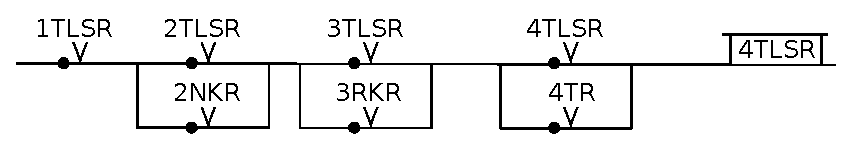
\includegraphics[keepaspectratio, width=100mm]{fig1.eps}
    \begin{displaymath}
      t_{\text{\it TLSR}_{4T}} =
      (\text{\it TLSR}_{1T} \vee \circ) \wedge
      \Bigl(\bigl\{(\text{\it TLSR}_{2T} \vee
      {\text{\it NKR}_{\#2}}^?), (\text{\it TLSR}_{3T} \vee
      {\text{\it RKR}_{\#3}}^?)\bigr\} \wedge (\text{\it TLSR}_{4T} \vee
      \text{\it TR}_{4}) \Bigr)
    \end{displaymath}
    \caption{interlocking logic example 1}
    \label{fig_of_instance_ex1}
  \end{center}
\end{figure}

Then we define some predicators and metrics on $\mathbb{T}$ as follows.

\begin{Definition}[grand terms]
  We define the set of grand terms of a given term $t \in \mathbb{T}$ as
  follows.
  \begin{displaymath}
    \mathpzc{gnd}(t) := \left\{\begin{array}{l}
      \{t_0\} \quad \text{\it if}\ t = t_0\
       \text{\it s.t.}\ (t_0,\mathcal{R}_0) \in \Gamma_{gnd}  \\
      \{t_1\} \quad \text{\it if}\ t = t_1\
       \text{\it s.t.}\ (t_1,\mathcal{R}_1) \in \Gamma_{def}  \\
      \mathpzc{gnd}(t_1) \cup \mathpzc{gnd}(t_2) \quad \text{\it if}\ t = t_1
       \wedge t_2\ \text{\it or}\ t_1 \vee t_2  \\
      \bigl\{ \{\} \bigr\} \quad \text{\it if}\ t = \{\}  \\
       \bigcup_{j=1}^{n}\mathpzc{gnd}(t_j) \quad \text{\it if}\
      t = \{t_1 \cdots t_n\}\ \text{\it or}\ [t_1 \cdots t_n]\ \text{\it or}\
       \langle t_1 \cdots t_n \rangle\ \text{\it s.t.}\ n \ge 1  \\
      \{\circ\} \quad \text{\it if}\ t = \circ  \\
       \mathpzc{gnd}(t_1) \quad \text{\it if}\ t = t_1^?\ \text{\it or}\
      t = t_1^{\leftarrow}\ \text{\it or}\ t = t_1^{\rightarrow}
    \end{array}\right.
  \end{displaymath}
\end{Definition}


\begin{Definition}[subterms]
  We define the set of subterms of a given term $t \in \mathbb{T}$ as
  follows.
  \begin{displaymath}
    \begin{array}{lll}
      \mathpzc{sub}(t) &:=
      & \left\{ \begin{array}{ll}
          \{t \}  &
           \text{\it if}\;
            \left\{ \! \begin{array}{l}
              t = t_0\ \text{\it s,t.}\
               (t_0, \mathcal{R}_0) \in \Gamma_{gnd}  \\
              t = t_1\ \text{\it s.t.}\
               (t_1, \mathcal{R}_1) \in \Gamma_{def}  \\
              t = \{\}  \\
              t = \circ
            \end{array} \right.  \\
          \{t \} \cup \bigl(\mathpzc{sub}(t_1) \cup \mathpzc{sub}(t_2)
           \bigr)  &
           \text{\it if}\;\; t = t_1 \wedge t_2,\ t_1 \vee t_2  \\
          \{t \} \cup \bigl(\bigcup^{n}_{j=1} \mathpzc{sub}(t_j) \bigr)  &
           \text{\it if}\;\; t = \{t_1 \cdots t_n \},
            \ [t_1 \cdots t_n ], \ \langle t_1 \cdots t_n \rangle  \\
          \{{t_1}^? \} \cup \mathpzc{sub}(t_1)  &
           \text{\it if}\;\; t = {t_1}^?  \\
          \{{t_1}^\leftarrow \} \cup \mathpzc{sub}(t_1)  &
           \text{\it if}\;\; t = {t_1}^\leftarrow \\
          \{{t_1}^\rightarrow \} \cup \mathpzc{sub}(t_1)  &
           \text{\it if}\;\; t = {t_1}^\rightarrow
        \end{array} \right.
    \end{array}
  \end{displaymath}
\end{Definition}


\begin{Definition}[term size]
  We define size of a given term $t \in \mathbb{T}$ as follow.
  \begin{displaymath}
    \begin{array}{lll}
      \mathpzc{size}(t) &:=
      & \left\{ \begin{array}{ll}
          1  & \text{\it if}\;
                \left\{ \! \begin{array}{l}
                  t = t_0\ \text{\it s,t.}\
                   (t_0, \mathcal{R}_0) \in \Gamma_{gnd}  \\
                  t = t_1\ \text{\it s.t.}\
                   (t_1, \mathcal{R}_1) \in \Gamma_{def}  \\
                  t = \{\}  \\
                  t = \circ
                \end{array} \right.  \\
          \bigl(\mathpzc{size}(t_1) + \mathpzc{size}(t_2) \bigr) + 1  &
           \text{\it if}\;\; t = t_1 \wedge t_2,\ t_1 \vee t_2  \\
          \bigl(\sum_{j=1}^{n} \mathpzc{size}(t_j) \bigr) + 1  &
           \text{\it if}\;\; t = \{t_1 \cdots t_n \},
            \ [t_1 \cdots t_n ], \ \langle t_1 \cdots t_n \rangle  \\
          \mathpzc{size}(t_1) + 1  &
           \text{\it if}\; \left\{ \! \begin{array}{l}
             t = {t_1}^?  \\
             t = {t_1}^\leftarrow \\
             t = {t_1}^\rightarrow
           \end{array} \right.
        \end{array} \right.
    \end{array}
  \end{displaymath}
\end{Definition}


\begin{Property}
  \label{self_similarity_on_subterms}
  \[ \mathpzc{sub}(t') \subseteq \mathpzc{sub}(t)\ \text{\it where}\
      t' \in \mathpzc{sub}(t)
  \]
  \begin{Proof}
    Proof is simple induction on sturcture of $t$.
    Here we show the proof only for the most significant case.
    
    Case $\{t_1, \cdots t_n\}$:
    We suppose $\mathpzc{sub}\bigl(\{t_1, \cdots t_n\} \bigr) =
    \bigl\{\{t_1, \cdots t_n\} \bigr\} \cup
    \bigl(\bigcup_{j=1}^n \mathpzc{sub}(t_j) \bigr)$ from def. of
    $\mathpzc{sub}$. For the case of $t'$ comming from
    $\mathpzc{sub}(t_j)$, i.e. $t' \in \mathpzc{sub}(t_j) \subseteq
    \mathpzc{sub}\bigl(\{t_1, \cdots t_n\} \bigr)$, we say
    $\mathpzc{sub}(t') \subseteq \mathpzc{sub}(t_j)$ from
    induction hypothesis.
    $\Box$
  \end{Proof}
\end{Property}


\begin{Definition}[patterns]
  We define the patterns $\mathcal{R}$ range over $\mathbb{R}$ as follow.
  \[ \mathcal{R} \;\stackrel{\mathrm{def}}{:=}\!
  \begin{array}[t]{l}
    \mathcal{R}_0 \ \text{\it s.t.}\; (t_0, \mathcal{R}_0) \!\in\!
     \Gamma_{gnd}\ |\ 
    \mathcal{R}_1\ \text{\it s.t.}\; (t_1, \mathcal{R}_1) \!\in\!
     \Gamma_{def}\ |\
    \mathcal{R}_1 \wedge \mathcal{R}_2 \ |\
     \mathcal{R}_1 \vee \mathcal{R}_2 \ |  \\
    {\mathcal{R}_1}^* \ |\ {\mathcal{R}_1}^+ \ |\
    {\mathcal{R}_1}^\downarrow \ |\ {\mathcal{R}_1}^? \ |\
    (\mathcal{R}_1 | \mathcal{R}_2)
  \end{array}
  \]
\end{Definition}

Intuitively we regard patterns as descripter of the set of specific terms,
i.e. $\mathcal{R}_{\text{\it TLSR}}$ has
$\text{\it TLSR}_{2T}, \text{\it TLSR}_{3T}, \text{\it TLSR}_{4T}, \cdots$
and $(\mathcal{R}_{\text{\it NKR}} | \mathcal{R}_{\text{\it RKR}})$ does
$\text{\it NKR}_{\#2}, \text{\it NKR}_{\#3}, \cdots$ , and
$\mathcal{R}_{\text{\it TLSR}} \vee (\mathcal{R}_{\text{\it NKR}} |
\mathcal{R}_{\text{\it RKR}})$ is 
$\text{\it TLSR}_{2T} \vee \text{\it NKR}_{\#2}$ so forth.

We also can describe arbitrary patterns to express any of terms belonging
to them. Follwing is one of example of pattern matching comming from
Figure \ref{fig_of_instance_ex1}.

\begin{figure}[htbp]
  \begin{center}
    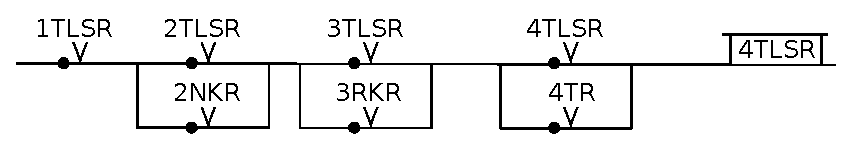
\includegraphics[keepaspectratio, width=100mm]{fig1.eps}
    \begin{displaymath}
      (\text{\it TLSR}_{1T} \vee \circ) \wedge \Bigl(\bigl\{(
      \text{\it TLSR}_{2T} \vee {\text{\it NKR}_{\#2}}^?),
      (\text{\it TLSR}_{3T} \vee {\text{\it RKR}_{\#3}}^?)\bigr\} \wedge
      (\text{\it TLSR}_{4T} \vee \text{\it TR}_{4}) \Bigr) :
      \mathcal{R}_{\text{\it TLSR}_{4T}}
    \end{displaymath}
    \begin{displaymath}
      \text{\it where}\;\; \mathcal{R}_{\text{\it TLSR}_{4T}} =
      \bigl(\text{\it TLSR} \vee {(\text{\it NKR} | \text{\it RKR})}^?
      \bigr) \wedge \Bigl(\bigl(\text{\it TLSR} \vee
      {(\text{\it NKR} | \text{\it RKR})}^? \bigr)^* \wedge
      (\text{\it TLSR} \vee \text{\it TR}) \Bigr)
    \end{displaymath}
    \caption{pattern of interlocking logic example 1}
    \label{fig_of_pattern_ex1}
  \end{center}
\end{figure}

Here we wrote $\mathcal{R}_{\text{\it XXX}}$ as $\text{\it XXX}$ in
shorthand, e.g. $\text{\it TLSR}$ as $\mathcal{R}_{\text{\it TLSR}}$. And
we write $t : \mathcal{R}$ with the intention of that $t$ matches
the pattern of $\mathcal{R}$, therefore
$t_{\text{\it TLSR}_{4T}} : \mathcal{R}_{\text{\it TLSR}_{4T}}$ means that
$t_{\text{\it TLSR}_{4T}}$ matches the pattern of
$\mathcal{R}_{\text{\it TLSR}_{4T}}$ where
$t_{\text{\it TLSR}_{4T}} =
(\text{\it TLSR}_{1T} \vee \circ) \wedge \Bigl(\bigl\{(\text{\it TLSR}_{2T}
\vee {\text{\it NKR}_{\#2}}^?), (\text{\it TLSR}_{3T} \vee {
\text{\it RKR}_{\#3}}^?)\bigr\} \wedge (\text{\it TLSR}_{4T} \vee
\text{\it TR}_{4}) \Bigr)$ as Figure \ref{fig_of_pattern_ex1}.

Consequently, we define the entity holding the correspondence between
term $t \in \mathbb{T}$ and patterns $\mathcal{R} \in \mathbb{R}$, as
binding and some related properties.

\begin{Definition}[binding]
  We define a set of pairs of $(t, \mathcal{R})$ where
  $t \in \mathbb{T}$ and $\mathcal{R} \in \mathbb{R}$, i.e.
  $\bigl\{(t, \mathcal{R}) \ |\ t \in \mathbb{T},\
  \mathcal{R} \in \mathbb{R} \bigr\}$, as binding ranging over $\Gamma$.
\end{Definition}


\begin{Definition}[binding domain]
  We define a set of terms $t$ comming from $\Gamma$ s.t.
  $\bigl\{ t \ |\ (t, \mathcal{R}) \in \Gamma \bigr\}$, as
  $\mathpzc{Dom}(\Gamma)$.
  \[ \mathpzc{Dom}(\Gamma) \,\stackrel{\mathrm{def}}{:=}\,
      \bigl\{ t \ |\ (t, \mathcal{R}) \in \Gamma \bigr\}
  \]
\end{Definition}


We easily find some properties on $\mathpzc{Dom}(\Gamma)$ as follows.


\begin{Property} \label{dom_bin_join}
  \[ \mathpzc{Dom}(\Gamma_1 \cup \Gamma_2) =
      \mathpzc{Dom}(\Gamma_1) \cup \mathpzc{Dom}(\Gamma_2)
  \]
  \begin{Proof}
    Proof is dirctrly from def. of $\mathpzc{Dom}$.
    
    $\mathpzc{Dom}(\Gamma_1 \cup \Gamma_2) \subseteq
    \mathpzc{Dom}(\Gamma_1) \cup \mathpzc{Dom}(\Gamma_2)$:
    From def. of $\mathpzc{Dom}$, we suppose that
    $t \in \mathpzc{Dom}(\Gamma_1 \cup \Gamma_2) =
    \bigl\{t' \ |\ (t', \mathcal{R}') \in (\Gamma_1 \cup \Gamma_2)
    \bigr\}$, then $t$ is $t'_1$ s.t. $(t'_1, \mathcal{R}'_1) \in \Gamma_1$
    or $t'_2$ s.t. $(t'_2, \mathcal{R}'_2) \in \Gamma_2$, which means
    $t \in \mathpzc{Dom}(\Gamma_1)$ or $t \in \mathpzc{Dom}(\Gamma_2)$ from
    def. of $\mathpzc{Dom}$. Hence
    $t \in \bigl(\mathpzc{Dom}(\Gamma_1) \cup \mathpzc{Dom}(\Gamma_2) \bigr)$.
    
    $\mathpzc{Dom}(\Gamma_1 \cup \Gamma_2) \supseteq
    \mathpzc{Dom}(\Gamma_1) \cup \mathpzc{Dom}(\Gamma_2)$:
    Now we suppose $t \in \bigl(\mathpzc{Dom}(\Gamma_1) \cup
    \mathpzc{Dom}(\Gamma_2) \bigr)$. Then from def. of $\mathpzc{Dom}$,
    $t$ belongs to $\Bigl(\bigl\{ t'_1 \ |\ (t'_1, \mathcal{R}'_1) \!\in\!
    \Gamma_1 \bigr\} \cup \bigl\{ t'_2 \ |\ (t'_2, \mathcal{R}'_2) \!\in\!
    \Gamma_2 \bigr\} \Bigr)$, which implies that
    $t$ is in $\bigl\{ t'_1 \ |\ (t'_1, \mathcal{R}'_1) \in \Gamma_1 \bigr\}$
    or $\bigl\{ t'_2 \ |\ (t'_2, \mathcal{R}'_2) \in \Gamma_2 \bigr\}$.
    Here we assume $t \in \bigl\{ t'_1 \ |\ (t'_1, \mathcal{R}'_1) \in
    \Gamma_1 \bigr\} \subseteq \bigl\{ t'' \ |\ (t'', \mathcal{R}'') \in
    (\Gamma_1 \cup \Gamma_2) \bigr\} = \mathpzc{Dom}(\Gamma_1 \cup
    \Gamma_2)$, and the counterpart case is also. Hence
    we can conclude that $t$ is also in
    $\bigl\{ t' \ |\ (t', \mathcal{R}') \in (\Gamma_1 \cup \Gamma_2)
    \bigr\} = \mathpzc{Dom}(\Gamma_1 \cup \Gamma_2)$, from def. of
    $\mathpzc{Dom}$.
    $\Box$
  \end{Proof}
\end{Property}


\begin{Property} \label{dom_mul_join}
  \[ \mathpzc{Dom}\Biggl(\bigcup_{j=1}^{n} \Gamma_j \Biggr) =
      \bigcup_{j=1}^{n} \mathpzc{Dom}(\Gamma_j)
  \]
  \begin{Proof}
    Proof is induction on $n$, as num. of
    $\, \Gamma_j$ s.t. $\mathpzc{Dom}(\Gamma_j)$.
    
    B.C.): $n = 1$: Trivial.
    $n = 2$: From Property \ref{dom_bin_join},
    $\mathpzc{Dom}(\Gamma_1 \cup \Gamma_2) = \mathpzc{Dom}(\Gamma_1) \cup
    \mathpzc{Dom}(\Gamma_2)$.
    
    I.S.): $n \ge 3$: $\mathpzc{Dom}\bigl(\bigcup_{j=1}^{n} \Gamma_j \bigr)
    = \mathpzc{Dom}\bigl(\Gamma_1 \cup \bigcup_{j=2}^{n} \Gamma_j \bigr) =
    \mathpzc{Dom}(\Gamma_1) \cup \mathpzc{Dom}\bigl(
    \bigcup_{j=2}^{n} \Gamma_j \bigr)$, from Property \ref{dom_bin_join}.
    Consequently we find that $\mathpzc{Dom}(\Gamma_1) \cup
    \mathpzc{Dom}\bigl(\bigcup_{j=2}^{n} \Gamma_j \bigr) =
    \mathpzc{Dom}(\Gamma_1) \cup \bigl(\bigcup_{j=2}^{n}
    \mathpzc{Dom}(\Gamma_j) \bigr)$, by induction hypothesis. Hence
    $\mathpzc{Dom}\bigl(\bigcup_{j=1}^{n} \Gamma_j) =
    \mathpzc{Dom}(\Gamma_1) \cup
    \bigl(\bigcup_{j=2}^{n} \mathpzc{Dom}(\Gamma_j) \bigr) =
    \bigcup_{j=1}^{n} \mathpzc{Dom}(\Gamma_j)$.
    $\Box$
  \end{Proof}
\end{Property}


\pagebreak
\begin{Definition}[matching rules on pure canonical terms]
  We define the matching rules on canonical terms as follow,
  where canonical terms $t$ range over $\mathbb{T}$, and patterns
  $\mathcal{R}$ over $\mathbb{R}$.
  
  \begin{displaymath}
    \begin{array}{c}
      
      \begin{array}{rl}
        \begin{array}{rl}
          \dfrac{
            \dfrac{}{
              \raisebox{0.6ex}[2.3ex][0ex]{
                $(t_0, \mathcal{R}_0) \!\in\! \Gamma_{gnd}$
              }
            }
          }{
            \bigl\{(t_0, \mathcal{R}_0) \bigr\} \vdash t_0 : \mathcal{R}_0
          }  &  \!\! \text{\it (T-Atom0-canon)}
        \end{array}

        & \begin{array}{rl}
          \dfrac{
            \dfrac{}{
              \raisebox{0.6ex}[2.3ex][0ex]{
                $(t_1, \mathcal{R}_1) \!\in\! \Gamma_{def}$
              }
            }
          }{
            \bigl\{(t_1, \mathcal{R}_1) \bigr\} \vdash t_1 : \mathcal{R}_1
          }  &  \!\! \text{\it (T-Atom1-canon)}
          \end{array}
      \end{array}  \\
      \\
      
      \begin{array}{rl}
        \dfrac{
          \begin{array}{c}
            \Gamma_1 \vdash t_1 : \mathcal{R}_1
             \quad \Gamma_2 \vdash t_2 : \mathcal{R}_2
              \quad \mathpzc{Dom}(\Gamma_1) \cap \mathpzc{Dom}(\Gamma_2)
              = \phi  \\
              t_1 \wedge t_2 \not\in \bigl(\mathpzc{Dom}(\Gamma_1) \cup
               \mathpzc{Dom}(\Gamma_2) \bigr)
          \end{array}
        }{
          \bigl\{(t_1 \wedge t_2, \mathcal{R}_1 \wedge \mathcal{R}_2)
           \bigr\} \cup (\Gamma_1 \cup \Gamma_2) \vdash
            t_1 \wedge t_2 : \mathcal{R}_1 \wedge \mathcal{R}_2
        }  &  \text{\it (T-Cas-canon)}  \\
        \\
        
        \dfrac{
          \begin{array}{c}
            \Gamma_1 \vdash t_1 : \mathcal{R}_1
             \quad \Gamma_2 \vdash t_2 : \mathcal{R}_2
              \quad \mathpzc{Dom}(\Gamma_1) \cap \mathpzc{Dom}(\Gamma_2)
               = \phi  \\
            t_1 \vee t_2 \not\in \bigl(\mathpzc{Dom}(\Gamma_1) \cup
             \mathpzc{Dom}(\Gamma_2) \bigr)
          \end{array}
        }{
          \bigl\{(t_1 \vee t_2, \mathcal{R}_1 \vee \mathcal{R}_2) \bigr\}
           \cup (\Gamma_1 \cup \Gamma_2) \vdash
            t_1 \vee t_2 : \mathcal{R}_1 \vee \mathcal{R}_2
        }  &  \text{\it (T-Par-canon)}
      \end{array}  \\
      \\
      
      \begin{array}{rl}
        \left. \begin{array}{rl}
          \dfrac{
          }{
            \Bigl\{\bigl(\{\}, {\mathcal{R}_1}^* \bigr) \Bigr\} \vdash
             \{\}: {\mathcal{R}_1}^*
              \quad \mathcal{R}_1\,\text{\it is}\, \text{\it Any}
          }  &  (\text{\it nil}\,)  \\
          \\
          \dfrac{
            \begin{array}{c}
              \Gamma_1 \vdash t_1 : \mathcal{R}_1 \,\cdots\,
               \Gamma_n \vdash t_n : \mathcal{R}_1,\
                \text{\it where}\ n \ge 1  \\
              \mathpzc{Dom}(\Gamma_j) \!\cap\! \mathpzc{Dom}(\Gamma_k) \!=\!
               \phi \ \text{\it s.t.}\; j \!\neq\! k
              \quad \{t_1 \cdots t_n \} \not\in
               \bigcup_{j=1}^{n}\mathpzc{Dom}(\Gamma_j)
            \end{array}
          }{
            \Bigl\{\bigl(\{t_1 \cdots t_n \}, {\mathcal{R}_1}^* \bigr)
             \Bigr\} \cup {\displaystyle \bigcup_{j = 1}^{n}} \Gamma_j
              \vdash \{t_1 \cdots t_n \} : {\mathcal{R}_1}^*
          }  &  (\infty)
        \end{array} \right\}  &  \text{\it (T-Cat0-canon)}
      \end{array}  \\
      \\
      
      \begin{array}{rl}
        \dfrac{
          \begin{array}{c}
            \Gamma_1 \vdash t_1 : \mathcal{R}_1 \,\cdots\,
             \Gamma_n \vdash t_n : \mathcal{R}_1,\
              \text{\it where}\ n \ge 1 \\
            \mathpzc{Dom}(\Gamma_j) \cap \mathpzc{Dom}(\Gamma_k) = \phi
             \ \text{\it s.t.}\; j \!\neq\! k
            \quad [t_1 \cdots t_n ] \not\in \bigcup_{j=1}^{n}
             \mathpzc{Dom}(\Gamma_j)
          \end{array}
        }{
          \Bigl\{\bigl([t_1 \cdots t_n], {\mathcal{R}_1}^+ \bigr) \Bigr\}
           \cup {\displaystyle \bigcup_{j = 1}^{n}} \Gamma_j
            \vdash [t_1 \cdots t_n] : {\mathcal{R}_1}^+
        }  &  \text{\it (T-Cat1-canon)}
      \end{array}  \\
      \\
      
      \begin{array}{rl}
        \dfrac{
          \begin{array}{c}
            \Gamma_1 \vdash t_1 : \mathcal{R}_1 \,\cdots\,
             \Gamma_n \vdash t_n : \mathcal{R}_1\
              \text{\it where}\ n \ge 1 \\
            \mathpzc{Dom}(\Gamma_j) \cap \mathpzc{Dom}(\Gamma_k) = \phi
             \ \text{\it s.t.}\; j \!\neq\! k
            \quad \langle t_1 \cdots t_n \rangle \not\in \bigcup_{j=1}^{n}
             \mathpzc{Dom}(\Gamma_j)
          \end{array}
        }{
          \Bigl\{\bigl(\langle t_1 \cdots t_n \rangle,
          {\mathcal{R}_1}^\downarrow \bigr) \Bigr\}
          \cup {\displaystyle \bigcup_{j = 1}^{n}} \Gamma_j \vdash
          \langle t_1 \cdots t_n \rangle : {\mathcal{R}_1}^\downarrow
        }  &  \text{\it (T-Dup-canon)}
      \end{array}  \\
      
    \end{array}
  \end{displaymath}
  
  \begin{displaymath}
    \begin{array}{c}
      
      \begin{array}{rl}
        \left. \begin{array}{rl}
          \dfrac{
          }{
            \bigl\{(\circ, {\mathcal{R}_1}^? ) \bigr\} \vdash
             \circ : {\mathcal{R}_1}^?
              \quad \mathcal{R}_1 \,\text{\it is}\, \text{\it Any}
          }  &  (\text{\it nil}\,)  \\
          \\
          \dfrac{
            \Gamma_1 \vdash t_1 : \mathcal{R}_1
            \quad {t_1}^? \not\in \mathpzc{Dom}(\Gamma_1)
          }{
            \bigl\{({t_1}^?, {\mathcal{R}_1}^?) \bigr\} \cup \Gamma_1 \vdash
                   {t_1}^? : {\mathcal{R}_1}^?
          }  &  (\text{\it sol}\,)
        \end{array} \right\}  &  \text{\it (T-Opt-canon)}
      \end{array}  \\
      
      \\
      \begin{array}{rl}
        \left. \begin{array}{rl}
          \dfrac{
            \Gamma_1 \vdash t_1 : \mathcal{R}_1
            \quad \mathcal{R}_2 \,\text{\it is}\, \text{\it Any}
            \quad {t_1}^{\leftarrow} \not\in \mathpzc{Dom}(\Gamma_1)
          }{
            \bigl\{({t_1}^\leftarrow, \mathcal{R}_1 | \mathcal{R}_2)
             \bigr\} \cup \Gamma_1 \vdash {t_1}^\leftarrow :
              \mathcal{R}_1 | \mathcal{R}_2
          }  &  (\text{\it L}\,)  \\
          \\
          \dfrac{
            \mathcal{R}_1 \,\text{\it is}\, \text{\it Any}
            \quad \Gamma_1 \vdash t_1 : \mathcal{R}_2
            \quad {t_1}^{\rightarrow} \not\in \mathpzc{Dom}(\Gamma_1)
          }{
            \bigl\{({t_1}^{\rightarrow}, \mathcal{R}_1 | \mathcal{R}_2)
             \bigr\} \cup \Gamma_1 \vdash {t_1}^\rightarrow :
              \mathcal{R}_1 | \mathcal{R}_2
          }  &  (\text{\it R}\,)
        \end{array} \right\}  &  \text{\it (T-Alt-canon)}
      \end{array}  
    \end{array}
  \end{displaymath}  
\end{Definition}


\vspace{5mm}
From def. of pattern matching rules, next 2 lemmas are straitforward.

\begin{Lemma}{termination on canonical pattern matching.}
  \label{termination_on_canonical_matching}
  \[ \Gamma \vdash t : \mathcal{R}\ \text{\it has termination.}
  \]
  \begin{Proof}
    Proof is directly structual induction on $\mathcal{R}$ of
    $\Gamma \vdash t : \mathcal{R}$.
    $\Box$
  \end{Proof}
\end{Lemma}


\begin{Property}
  \label{dom_of_Gamma}
  \[ \mathpzc{Dom}(\Gamma) = \mathpzc{sub}(t)\ \text{\it where}\
      \Gamma \vdash t : \mathcal{R}.
  \]
  \begin{Proof}
    Proof is simple induction on structure of $t$ s.t.
    $\Gamma \vdash t : \mathcal{R}$.
    Here we show the proof only for the most significant case.
    
    Case (T-Cat0-canon-$\infty$): From def. of (T-Cat0-canon-$\infty$),
    we let
    $\Gamma = \Bigl\{\bigl(\{t_1 \cdots t_n \}, {\mathcal{R}_1}^* \bigr)
    \Bigr\} \cup \bigcup_{j = 1}^{n} \Gamma_j$. And from
    the facts of $\Gamma_1 \vdash t_1 : \mathcal{R}_1 \cdots
    \Gamma_n \vdash t_n : \mathcal{R}_1$ comming from def. of
    (T-Cat0-canon-$\infty$), we can find that
    $\mathpzc{Dom}(\Gamma_1) = \mathpzc{sub}(t_1) \cdots
    \mathpzc{Dom}(\Gamma_n) = \mathpzc{sub}(t_n)$ by I.H.
    Accounting on the fact of
    $\mathpzc{Dom}(\Gamma_1) \cup \cdots \cup \mathpzc{Dom}(\Gamma_n) =
    \bigcup_{j=1}^n \mathpzc{Dom}(\Gamma_j)$, we can express it as
    $\bigcup_{j=1}^n \mathpzc{Dom}(\Gamma_j) = \mathpzc{sub}(t_1)
    \cup \cdots \cup \mathpzc{sub}(t_n)$. By now we can show that
    $\mathpzc{Dom}(\Gamma) = \mathpzc{Dom}\biggl(\Bigl\{\bigl(
    \{t_1 \cdots t_n \}, {\mathcal{R}_1}^* \bigr) \Bigr\} \cup
    \bigcup_{j = 1}^{n} \Gamma_j \biggr) =
    \mathpzc{Dom}\biggl(\Bigl\{\bigl(\{t_1 \cdots t_n \}, {\mathcal{R}_1}^*
    \bigr) \Bigr\} \biggr) \cup
    \mathpzc{Dom}\bigl(\bigcup_{j = 1}^{n} \Gamma_j \bigr) =
    \bigl\{\{t_1 \cdots t_n \} \bigr\} \cup  \bigcup_{j = 1}^{n}
    \mathpzc{Dom}(\Gamma_j) = \bigl\{\{t_1 \cdots t_n \} \bigr\}
    \cup \bigl(\mathpzc{sub}(t_1) \cup \cdots \cup \mathpzc{sub}(t_n)
    \bigr) = \mathpzc{sub}\bigl(\{t_1 \cdots t_n\} \bigr)$ as desired,
    from def. of $\mathpzc{Dom}(\Gamma)$ and
    $\mathpzc{sub}\bigl(\{t_1 \cdots t_n\} \bigr)$.
    $\Box$
  \end{Proof}
\end{Property}


\begin{Property}
  \label{termsize_constraint_on_Gamma}
  \[ \mathpzc{size}(t) \ge \mathpzc{size}(t')\ \text{\it s.t.}\
      t' \in \mathpzc{Dom}(\Gamma),\ \text{\it where}\
       \Gamma \vdash t : \mathcal{R}.
  \]
  \begin{Proof}
    Proof is directly from def. of size of terms, with Property
    \ref{dom_of_Gamma}.
    $\Box$
  \end{Proof}
\end{Property}


Based on the matching rules above, we show the matching of
$t_{\text{\it TLSR}_{4T}} : \mathcal{R}_{\text{\it TLSR}}$ introduced
by Figure \ref{fig_of_pattern_ex1} as
Figure \ref{fig_of_patternmatching_ex1}.


\begin{landscape}
  \begin{figure}
  \begin{tiny}
  \begin{prooftree}
    \AxiomC{}
    \UnaryInfC{$(\text{\it TLSR}_{2T}, \text{\it TLSR})
      \in \Gamma_{\text{\it gnd}}$}
    \LeftLabel{$(0)$}
    \UnaryInf$\Gamma_{10} \vdash \fCenter\
      \text{\it TLSR}_{2T} : \text{\it TLSR}$
    \noLine
    \def\extraVskip{0.3pt}  
    \UnaryInf$\Gamma_{10} = \fCenter\
      \{\text{\it TLSR}_{2T}, \text{\it TLSR}\}$
    \def\extraVskip{2pt}
    
    \AxiomC{}
    \UnaryInfC{$(\text{\it NKR}_{\#2}, \text{\it NKR})
      \in \Gamma_{\text{\it gnd}}$}
    \LeftLabel{$(0)$}
    \UnaryInf$\Gamma_{13} \vdash \fCenter\
      \text{\it NKR}_{\#2} : \text{\it NKR}$
    \noLine
    \def\extraVskip{0.3pt}  
    \UnaryInf$\Gamma_{13} = \fCenter\
      \{\text{\it NKR}_{\#2}, \text{\it NKR}\}$
    \def\extraVskip{2pt}

    \LeftLabel{$(L)$}
    \UnaryInf$\Gamma_{12} \vdash \fCenter\
    \text{\it NKR}_{\#2} : \text{\it NKR} | \text{\it RKR}$
    \noLine
    \def\extraVskip{0.3pt}  
    \UnaryInf$\Gamma_{12} = \fCenter\ 
    \{\text{\it NKR}_{\#2}, \text{\it NKR} | \text{\it RKR}\}
    \cup \Gamma_{13}$
    \def\extraVskip{2pt}
    
    \LeftLabel{$(?)$}
    \UnaryInf$\Gamma_{11} \vdash \fCenter\
      {\text{\it NKR}_{\#2}}^? : {(\text{\it NKR} | \text{\it RKR})}^?$
    \noLine
    \def\extraVskip{0.3pt}  
    \UnaryInf$\Gamma_{11} = \fCenter\ \bigl\{
    {\text{\it NKR}_{\#2}}^?, {(\text{\it NKR} | \text{\it RKR})}^?\bigr\}
    \cup \Gamma_{12}$
    \def\extraVskip{2pt}
    
    \LeftLabel{$(\text{\it Par})$}
    \BinaryInf$\Gamma_8 \vdash \fCenter\
      \text{\it TLSR}_{2T} \vee {\text{\it NKR}_{\#2}}^? :
      \text{\it TLSR} \vee {(\text{\it NKR} | \text{\it RKR})}^?$
    \noLine
    \def\extraVskip{0.3pt}  
    \UnaryInf$\Gamma_8 = \fCenter\
      \bigl\{\text{\it TLSR}_{2T} \vee {\text{\it NKR}_{\#2}}^?,
      \text{\it TLSR} \vee {(\text{\it NKR} | \text{\it RKR})}^?\bigr\} \cup
      (\Gamma_{10} \cup \Gamma_{11})$
    \def\extraVskip{2pt}
      
    \AxiomC{}
    \UnaryInfC{$(\text{\it TLSR}_{3T}, \text{\it TLSR})
      \in \Gamma_{\text{\it gnd}}$}
    \RightLabel{$(0)$}
    \UnaryInf$\Gamma_{14} \vdash \fCenter\
      \text{\it TLSR}_{3T} : \text{\it TLSR}$
    \noLine
    \def\extraVskip{0.3pt}
    \UnaryInf$\Gamma_{14} = \fCenter\
      \{\text{\it TLSR}_{3T}, \text{\it TLSR}\}$
    \def\extraVskip{2pt}
    
    \AxiomC{}
    \UnaryInfC{$(\text{\it RKR}_{\#3}, \text{\it RKR})
      \in \Gamma_{\text{\it gnd}}$}
    \RightLabel{$(0)$}
    \UnaryInf$\Gamma_{17} \vdash \fCenter\
      \text{\it RKR}_{\#3}, \text{\it RKR}$
    \noLine
    \def\extraVskip{0.3pt}
    \UnaryInf$\Gamma_{17} = \fCenter\
      \{\text{\it RKR}_{\#3}, \text{\it RKR}\}$
    \def\extraVskip{2pt}
    
    \RightLabel{$(R)$}
    \UnaryInf$\Gamma_{16} \vdash \fCenter\
    \text{\it RKR}_{\#3} : \text{\it NKR} | \text{\it RKR}$
    \noLine
    \def\extraVskip{0.3pt}
    \UnaryInf$\Gamma_{16} = \fCenter\
    \{\text{\it RKR}_{\#3}, \text{\it NKR} | \text{\it RKR}\} \cup
    \Gamma_{17}$
    \def\extraVskip{2pt}
    
    \RightLabel{$(?)$}
    \UnaryInf$\Gamma_{15} \vdash \fCenter\
    {\text{\it RKR}_{\#3}}^? : {(\text{\it NKR} | \text{\it RKR})}^?$
    \noLine
    \def\extraVskip{0.3pt}
    \UnaryInf$\Gamma_{15} = \fCenter\
    \bigl\{{\text{\it RKR}_{\#3}}^?,
    {(\text{\it NKR} | \text{\it RKR})}^?\bigr\} \cup \Gamma_{16}$
    \def\extraVskip{2pt}
    
    \RightLabel{$(\text{\it Par})$}
    \BinaryInf$\Gamma_9 \vdash \fCenter\
      \text{\it TLSR}_{3T} \vee {\text{\it RKR}_{\#3}}^? :
      \text{\it TLSR} \vee {(\text{\it NKR} | \text{\it RKR})}^?$
    \noLine
    \def\extraVskip{0.3pt}
    \UnaryInf$\Gamma_9 = \fCenter\
      \bigl\{\text{\it TLSR}_{3T} \vee {\text{\it RKR}_{\#3}}^?,
      \text{\it TLSR} \vee {(\text{\it NKR} | \text{\it RKR})}^?\bigr\}
      \cup (\Gamma_{14} \cup \Gamma_{15})$
    \def\extraVskip{2pt}
    
    \RightLabel{$(\infty)$}
    \BinaryInf$\Gamma_6 \vdash \fCenter\
      \bigl\{(\text{\it TLSR}_{2T} \vee
      {\text{\it NKR}_{\#2}}^?), (\text{\it TLSR}_{3T} \vee
      {\text{\it RKR}_{\#3}}^?)\bigr\} :{\bigl(\text{\it TLSR} \vee
        {(\text{\it NKR} | \text{\it RKR})}^?\bigr)}^*$
    \noLine
    \def\extraVskip{0.3pt}
    \UnaryInf$\Gamma_6 = \fCenter\
      \Bigl\{\bigl\{(\text{\it TLSR}_{2T} \vee
      {\text{\it NKR}_{\#2}}^?), (\text{\it TLSR}_{3T} \vee
      {\text{\it RKR}_{\#3}}^?)\bigr\}, {\bigl(\text{\it TLSR} \vee
      {(\text{\it NKR} | \text{\it RKR})}^?\bigr)}^*\Bigr\} \cup
      (\Gamma_8 \cup \Gamma_9)$
    \def\extraVskip{2pt}
  \end{prooftree}
  
  \begin{prooftree}
    \noLine
    \AxiomC{}
    \UnaryInfC{$\Gamma_6 \vdash
      \bigl\{(\text{\it TLSR}_{2T} \vee
      {\text{\it NKR}_{\#2}}^?), (\text{\it TLSR}_{3T} \vee
      {\text{\it RKR}_{\#3}}^?)\bigr\} :{\bigl(\text{\it TLSR} \vee
      {(\text{\it NKR} | \text{\it RKR})}^?\bigr)}^*$}
    
    \AxiomC{}
    \UnaryInfC{$(\text{\it TLSR}_{4T}, \text{\it TLSR})
      \in \Gamma_{\text{\it gnd}}$}
    \LeftLabel{$(0)$}
    \UnaryInf$\Gamma_{18} \vdash \fCenter\
      \text{\it TLSR}_{4T} : \text{\it TLSR}$
    \noLine
    \def\extraVskip{0.3pt}
    \UnaryInf$\Gamma_{18} = \fCenter\
      \{\text{\it TLSR}_{4T}, \text{\it TLSR}\}$
    \def\extraVskip{2pt}
    
    \AxiomC{}
    \UnaryInfC{$(\text{\it TR}_{4}, \text{\it TR})
      \in \Gamma_{\text{\it gnd}}$}
    
    \LeftLabel{$(0)$}
    \UnaryInf$\Gamma_{19} \vdash \fCenter\
    \text{\it TR}_{4} : \text{\it TR}$
    \noLine
    \def\extraVskip{0.3pt}
    \UnaryInf$\Gamma_{19} = \fCenter\
    \{\text{\it TR}_{4}, \text{\it TR}\}$
    \def\extraVskip{2pt}
    
    \RightLabel{$(\text{\it Par})$}
    \BinaryInf$\Gamma_7 \vdash \fCenter\
      \text{\it TLSR}_{4T} \vee \text{\it TR}_{4} :
      \text{\it TLSR} \vee \text{\it TR}$
    \noLine
    \def\extraVskip{0.3pt}
    \UnaryInf$\Gamma_7 = \fCenter\
      \{\text{\it TLSR}_{4T} \vee \text{\it TR}_{4},
      \text{\it TLSR} \vee \text{\it TR}\} \cup
      (\Gamma_{18} \cup \Gamma_{19})$
    \def\extraVskip{2pt}
    
    \RightLabel{$(\text{\it Cas})$}
    \BinaryInf$\Gamma_3 \vdash \fCenter\
    \bigl\{(\text{\it TLSR}_{2T} \vee {\text{\it NKR}_{\#2}}^?),
    (\text{\it TLSR}_{3T} \vee {\text{\it RKR}_{\#3}}^?)\bigr\} \wedge
    (\text{\it TLSR}_{4T} \vee \text{\it TR}_{4}) : \bigl(
    \text{\it TLSR} \vee {(\text{\it NKR} | \text{\it RKR})}^? \bigr)^*
    \wedge (\text{\it TLSR} \vee \text{\it TR})$
    \noLine
    \def\extraVskip{0.3pt}
    \UnaryInf$\Gamma_3 = \fCenter\
    \Bigl\{\bigl\{(\text{\it TLSR}_{2T} \vee {\text{\it NKR}_{\#2}}^?),
    (\text{\it TLSR}_{3T} \vee {\text{\it RKR}_{\#3}}^?)\bigr\} \wedge
    (\text{\it TLSR}_{4T} \vee \text{\it TR}_{4}), \bigl(
    \text{\it TLSR} \vee {(\text{\it NKR} | \text{\it RKR})}^? \bigr)^*
    \wedge (\text{\it TLSR} \vee \text{\it TR})\Bigr\} \cup
    (\Gamma_6 \cup \Gamma_7)$
    \def\extraVskip{2pt}
  \end{prooftree}
    
  \begin{prooftree}
    \AxiomC{}
    \UnaryInfC{$\bigl(\text{\it TLSR}_{1T}, \text{\it TLSR}\bigr)
      \in \Gamma_{\text{\it gnd}}$}
      
    \LeftLabel{$(0)$}
    \UnaryInf$\Gamma_4 \vdash \fCenter\
      \text{\it TLSR}_{1T} : \text{\it TLSR}$
    \noLine
    \def\extraVskip{0.3pt}
    \UnaryInf$\Gamma_4 = \fCenter\
      \bigl\{\text{\it TLSR}_{1T}, \text{\it TLSR}\bigr\}$
    \def\extraVskip{2pt}
    
    \AxiomC{}
    \LeftLabel{$\bigl({\text{\it nil}}^?\bigr)$}
    \UnaryInf$\Gamma_5 \vdash \fCenter\
      \circ : {(\text{\it NKR} | \text{\it RKR})}^?$
    \noLine
    \def\extraVskip{0.3pt}
    \UnaryInf$\Gamma_5 = \fCenter\
      \bigl\{\circ, {(\text{\it NKR} | \text{\it RKR})}^?\bigr\}$
    \def\extraVskip{2pt}
    
    \RightLabel{$(\text{\it Par})$}
    \BinaryInf$\Gamma_2 \vdash \fCenter\
      \text{\it TLSR}_{1T} \vee \circ:
      \text{\it TLSR} \vee {(\text{\it NKR} | \text{\it RKR})}^?$
    \noLine
    \def\extraVskip{0.3pt}
    \UnaryInf$\Gamma_2 = \fCenter\
      \Bigl\{\text{\it TLSR}_{1T} \vee \circ,
      \text{\it TLSR} \vee {(\text{\it NKR} | \text{\it RKR})}^?\Bigr\}
      \cup (\Gamma_4 \cup \Gamma_5)$
    \def\extraVskip{2pt}
    
    \noLine
    \AxiomC{}
    \UnaryInfC{$\Gamma_3 \vdash
      \bigl\{(\text{\it TLSR}_{2T} \vee
      {\text{\it NKR}_{\#2}}^?), (\text{\it TLSR}_{3T} \vee
      {\text{\it RKR}_{\#3}}^?)\bigr\} \wedge (\text{\it TLSR}_{4T} \vee
      \text{\it TR}_{4}) : \bigl(
      \text{\it TLSR} \vee {(\text{\it NKR} | \text{\it RKR})}^? \bigr)^*
      \wedge (\text{\it TLSR} \vee \text{\it TR})$}
    
    \RightLabel{$(\text{\it Cas})$}
    \BinaryInf$\Gamma_1 \vdash \fCenter\
      (\text{\it TLSR}_{1T} \vee \circ) \wedge
      \Bigl(\bigl\{(\text{\it TLSR}_{2T} \vee
      {\text{\it NKR}_{\#2}}^?), (\text{\it TLSR}_{3T} \vee
      {\text{\it RKR}_{\#3}}^?)\bigr\} \wedge (\text{\it TLSR}_{4T} \vee
      \text{\it TR}_{4}) \Bigr) :
      \bigl(\text{\it TLSR} \vee {(\text{\it NKR} | \text{\it RKR})}^?
      \bigr) \wedge \Bigl(\bigl(
      \text{\it TLSR} \vee {(\text{\it NKR} | \text{\it RKR})}^? \bigr)^*
      \wedge (\text{\it TLSR} \vee \text{\it TR}) \Bigr)$
    \noLine
    \def\extraVskip{0.2pt}
    \UnaryInf$\Gamma_1 = \fCenter\
      \Biggl\{(\text{\it TLSR}_{1T} \vee \circ) \wedge
      \Bigl(\bigl\{(\text{\it TLSR}_{2T} \vee
      {\text{\it NKR}_{\#2}}^?), (\text{\it TLSR}_{3T} \vee
      {\text{\it RKR}_{\#3}}^?)\bigr\} \wedge (\text{\it TLSR}_{4T} \vee
      \text{\it TR}_{4}) \Bigr),
      \bigl(\text{\it TLSR} \vee {(\text{\it NKR} | \text{\it RKR})}^?
      \bigr) \wedge \Bigl(\bigl(
      \text{\it TLSR} \vee {(\text{\it NKR} | \text{\it RKR})}^? \bigr)^*
      \wedge (\text{\it TLSR} \vee \text{\it TR}) \Bigr) \biggr\} \cup
      (\Gamma_2 \cup \Gamma_3)$
    \def\extraVskip{2pt}
  \end{prooftree}
  \begin{flushright}
  legend
  $(0)$: $\text{\it (T-Atom0-canon)}$,
  $(\text{\it Cas})$: $\text{\it (T-Cas-canon)}$,
  $(\text{\it Par})$: $\text{\it (T-Par-canon)}$, 
  $(\infty)$: $\text{\it (T-Cat0-canon-$\infty$)}$,
  $\bigl({\text{\it nil}}^?\bigr)$: $\text{\it (T-Opt-canon-nil)}$,
  $(?)$: $\text{\it (T-Opt-canon-sol)}$,
  $(L)$: $\text{\it (T-Alt-canon-L)}$,
  $(R)$: $\text{\it (T-Alt-canon-R)}$.
  \end{flushright}
  \end{tiny}
  \caption{pattern matching of interlocking logic example 1}
  \label{fig_of_patternmatching_ex1}
  \end{figure}
\end{landscape}


\section{More flexible system}
We have developed the basic system in previous chapter,
but as you see, it's hard to use. Rigid discipline forces us to behave
strictly for expressions. In short, excessive strictness also
decreases its usability. E.g. $1+(2+3)$ and $(1+2)+3$ aren't identical
syntactically,
but it's natural to regard them as identical, since associativity has little
importance on same precedence operations. Similar to that, it's preferable
to match both instances of
$(\text{\it TLSR}_{1T} \vee \circ) \wedge \Bigl(\bigl\{
(\text{\it TLSR}_{2T} \vee {\text{\it NKR}_{\#2}}^?),
(\text{\it TLSR}_{3T} \vee {\text{\it RKR}_{\#3}}^?)\bigr\} \wedge
(\text{\it TLSR}_{4T} \vee \text{\it TR}_{4}) \Bigr)$ and
$\Bigl((\text{\it TLSR}_{1T} \vee \circ) \wedge \bigl\{
(\text{\it TLSR}_{2T} \vee {\text{\it NKR}_{\#2}}^?),
(\text{\it TLSR}_{3T} \vee {\text{\it RKR}_{\#3}}^?)\bigr\} \Bigr) \wedge
(\text{\it TLSR}_{4T} \vee \text{\it TR}_{4})$, but pattern of
$\bigl(\text{\it TLSR} \vee {(\text{\it NKR} | \text{\it RKR})}^? \bigr)
\wedge \Bigl(\bigl(\text{\it TLSR} \vee {(\text{\it NKR} | \text{\it RKR})}^?
\bigr)^* \wedge (\text{\it TLSR} \vee \text{\it TR}) \Bigr)$
matches with only former one since their associativity embedded in their
own structures. Accordingly, we hope to describe instances more simply, and
match them more flexible. For example it's preferable that we can express
more flexibly them above as
$\text{\it TLSR}_{1T} \wedge (\text{\it TLSR}_{2T} \vee
\text{\it NKR}_{\#2}) \wedge (\text{\it TLSR}_{3T} \vee
\text{\it RKR}_{\#3}) \wedge (\text{\it TLSR}_{4T} \vee
\text{\it TR}_{4})$, and matches with the pattern of
$\bigl(\text{\it TLSR} \vee {(\text{\it NKR} | \text{\it RKR})}^? \bigr)^*
\wedge (\text{\it TLSR} \vee \text{\it TR})$
by accounting on semantic meaming, but it's also impossible on
current system.

In this chapter, we bring our system more flexibility, and make it more
usable based on a well known type theoretical technology as polymorphism.

As first step, we define relations of intuitionistic equivalence over
terms, which allow us to regard distinct terms as equivalent, as follow.

\pagebreak
\begin{Definition}[intuitionistic equivalence over canonical terms]
  \label{equality_on_CANONICALS}
  We define the set of intuitionistic equivalence terms of $t$ as follows.
  We write $t \simeq t'$ if $t$ is intuitionistic equivalent to $t'$.
  \begin{displaymath}
    \begin{array}{c}
      
      \begin{array}{rl}
          \dfrac{
            \dfrac{}{
              \raisebox{0.5ex}[2.3ex][0ex]{$t \equiv t'$}
            }
          }{
            t \simeq t'
          }  &  (\text{\it Identity})
      \end{array}  \\
      \\
      
      \begin{array}{rl}
        \begin{array}{rl}
          \dfrac{
            t \simeq t'\
          }{
            t' \simeq t
          }  &  (\text{\it Symmetry})
        \end{array}
        
        & \begin{array}{rl}
            \dfrac{t_1 \simeq t_2 \quad t_2 \simeq t_3}{
              t_1 \simeq t_3
            }  &  (\text{\it Transitivity})
          \end{array}
      \end{array}  \\
      \\
      
      \begin{array}{ll}
        \begin{array}{rl}
          \dfrac{t_1 \simeq t'_1 \quad t_2 \simeq t'_2}{
            t_1 \!\wedge\! t_2 \simeq t'_1 \!\wedge\! t'_2
          }  &  (\text{\it Transparency-Cas})
        \end{array}
        
        & \begin{array}{rl}
            \dfrac{t_1 \simeq t'_1 \quad t_2 \simeq t'_2}{
              t_1 \!\vee\! t_2 \simeq t'_1 \!\vee\! t'_2
            }  &  (\text{\it Transparency-Par})
          \end{array}
      \end{array}  \\
      \\

      \begin{array}{ll}
        \begin{array}{rl}
          \dfrac{ t \simeq t_1 \wedge (t_2 \wedge t_3) }{
            t \simeq (t_1 \wedge t_2) \wedge t_3
          }  &  (\text{\it Associativity-Cas}_{\mathpzc{L}})
        \end{array}
        
        & \begin{array}{rl}
            \dfrac{t \simeq (t_1 \wedge t_2) \wedge t_3 }{
              t \simeq  t_1 \wedge (t_2 \wedge t_3)
            }  &  (\text{\it Associativity-Cas}_{\mathpzc{R}})
          \end{array}  \\
      \end{array}  \\
      \\
      
      \begin{array}{ll}
        \begin{array}{rl}
          \dfrac{ t \simeq (t_1 \vee t_2) \vee t_3 }{
            t \simeq t_1 \vee (t_2 \vee t_3)
          }  &  (\text{\it Associativity-Par}_{\mathpzc{L}})
        \end{array}      
        & \begin{array}{rl}
            \dfrac{t \simeq t_1 \vee (t_2 \vee t_3) }{
              t \simeq (t_1 \vee t_2) \vee t_3
            }  &  (\text{\it Associativity-Par}_{\mathpzc{R}})
          \end{array}
      \end{array}  \\
      \\
            
      \begin{array}{rl}
        \begin{array}{rl}
          \dfrac{ t \simeq t' }{ t \simeq \{t'\} }
          & (\text{\it Associativity-Cat0}_1)
        \end{array}
        & \begin{array}{rl}
            \dfrac{
              t \simeq t_1 \wedge \{t_2 \cdots t_n \}
            }{
              t \simeq \{t_1, t_2 \cdots t_n \}
            }  &  (\text{\it AssociativityH-Cat0}_\infty)
          \end{array}
      \end{array}  \\
      \\
      
      \begin{array}{rl}
        \begin{array}{rl}
          \dfrac{ t \simeq t' }{ t \simeq [t'] }
          & (\text{\it Associativity-Cat1}_1)
        \end{array}
        & \begin{array}{rl}
            \dfrac{
              t \simeq t_1 \wedge [t_2 \cdots t_n ]
            }{
              t \simeq [t_1, t_2 \cdots t_n ]
            }  &  (\text{\it AssociativityH-Cat1}_\infty)
          \end{array}
      \end{array}  \\
      \\

      \begin{array}{rl}
        \begin{array}{rl}
          \dfrac{ t \simeq t' }{ t \simeq \langle t' \rangle }
          & (\text{\it Associativity-Dup}_1)
        \end{array}
        & \begin{array}{rl}
            \dfrac{
              t \simeq t_1 \vee \langle t_2 \cdots t_n \rangle
            }{
              t \simeq \langle t_1, t_2 \cdots t_n \rangle
            }  &  (\text{\it AssociativityH-Dup}_\infty)
          \end{array}  \\
      \end{array}  \\
      \\
      
      \begin{array}{ll}
        \begin{array}{rl}
          \dfrac{ t \simeq \{\,\} \wedge t' }{
            t \simeq t'
          }  &  (\text{\it RevealH-Cas}_{\{\}})
        \end{array}
        & \begin{array}{rl}
            \dfrac{ t \simeq t' \wedge \{\,\} }{
              t \simeq t'
            }  &  (\text{\it RevealT-Cas}_{\{\}})
          \end{array}
      \end{array}  \\
      \\
      
      \begin{array}{ll}
        \begin{array}{rl}
          \dfrac{ t \simeq \circ \wedge t' }{
            t \simeq t'
          }  &  (\text{\it RevealH-Cas}_\circ)
        \end{array}
        & \begin{array}{rl}
            \dfrac{ t \simeq t' \wedge \circ }{
              t \simeq t'
            }  &  (\text{\it RevealT-Cas}_\circ)
          \end{array}
      \end{array}  \\
      \\
            
      \begin{array}{ll}
        \begin{array}{rl}
          \dfrac{ t \simeq \{\,\} \vee t' }{
            t \simeq t'
          }  &  (\text{\it RevealH-Par}_{\{\}})
        \end{array}
        & \begin{array}{rl}
            \dfrac{ t \simeq t' \vee \{\,\} }{
              t \simeq t'
            }  &  (\text{\it RevealT-Par}_{\{\}})
          \end{array}
      \end{array}  \\
      \\

      \begin{array}{ll}
        \begin{array}{rl}
          \dfrac{ t \simeq \circ \vee t' }{
            t \simeq t'
          }  &  (\text{\it RevealH-Par}_\circ)
        \end{array}
        & \begin{array}{rl}
            \dfrac{ t \simeq t' \vee \circ }{
              t \simeq t'
            }  &  (\text{\it RevealT-Par}_\circ)
          \end{array}
      \end{array}
      
    \end{array}
  \end{displaymath}
  
  \begin{displaymath}
    \begin{array}{c}
      

      
      \begin{array}{ll}
        \begin{array}{rl}
          \dfrac{ t \simeq t' }{
            t \simeq \{\,\} \wedge t'
          }  &  (\text{\it PhonyH-Cas}_{\{\}})
        \end{array}
        & \begin{array}{rl}
            \dfrac{ t \simeq t' }{
              t \simeq t' \wedge \{\,\}
            }  &  (\text{\it PhonyT-Cas}_{\{\}})
          \end{array}
      \end{array}  \\
      \\
      
      \begin{array}{ll}
        \begin{array}{rl}
          \dfrac{ t \simeq t' }{
            t \simeq \circ \wedge t'
          }  &  (\text{\it PhonyH-Cas}_\circ)
        \end{array}
        & \begin{array}{rl}
            \dfrac{ t \simeq t' }{
              t \simeq t' \wedge \circ
            }  &  (\text{\it PhonyT-Cas}_\circ)
          \end{array}
      \end{array}  \\
      \\
            
      \begin{array}{ll}
        \begin{array}{rl}
          \dfrac{ t \simeq t' }{
            t \simeq \{\,\} \vee t'
          }  &  (\text{\it PhonyH-Par}_{\{\}})
        \end{array}
        & \begin{array}{rl}
            \dfrac{ t \simeq t' }{
              t \simeq t' \vee \{\,\}
            }  &  (\text{\it PhonyT-Par}_{\{\}})
          \end{array}
      \end{array}  \\
      \\

      \begin{array}{ll}
        \begin{array}{rl}
          \dfrac{ t \simeq t' }{
            t \simeq \circ \vee t'
          }  &  (\text{\it PhonyH-Par}_\circ)
        \end{array}
        & \begin{array}{rl}
            \dfrac{ t \simeq t' }{
              t \simeq t' \vee \circ
            }  &  (\text{\it PhonyT-Par}_\circ)
          \end{array}
      \end{array}  \\
      \\
      
      \begin{array}{rll}
        \begin{array}{rl}
          \dfrac{
            t \simeq t'
          }{
            t \simeq {t'}^?
          }  &  (\text{\it Optional})
        \end{array}

        & \begin{array}{rl}
            \dfrac{
              t \simeq t'
            }{
              t \simeq {t'}^\leftarrow
            }  &  (\text{\it Alt-L})
          \end{array}
        
        & \begin{array}{rl}
            \dfrac{
              t \simeq t'
            }{
              t \simeq {t'}^\rightarrow
            }  &  (\text{\it Alt-R})
          \end{array}
      \end{array}
      
    \end{array}
  \end{displaymath}
\end{Definition}


\vspace{\baselineskip}
Then we extend the definition of judgement to use the set of equivalent
terms given from above definition of $t \simeq t_{\text{\it equ}}$.

\begin{Definition}[binding pentagram]
  We extend the definition of bindings $\Gamma$ defined above,
  and we call the extended ones range over $\Delta$  as binding pentagram.
  \begin{displaymath}
    \Delta \;\stackrel{\mathrm{def}}{:=}\;
     \bigl\{(t, t_{\text{\it equ}}, \mathcal{R},
      \mathcal{S}_{\mathpzc{fin}}, \Delta') \bigr\} \cup \Delta'
      \begin{array}[t]{l}
        \text{\it s.t.}\ \Delta \!\vdash\! t \triangleright \!\mathcal{R} \\
        \text{\it where}\ \begin{array}[t]{l}
         t \simeq t_{\text{\it equ}}  \\
        \mathcal{S}_{\mathpzc{fin}}\in \{\text{\it gnd},
         \text{\it def}, \wedge, \vee, \text{\it nil}, \text{\it sol},
          \infty, \text{\it L}, \text{\it R}\}
        \end{array}
      \end{array}
  \end{displaymath}
  We still regard extended bindings $\Delta$ as the mapping of
  $\mathbb{T} \mapsto \Delta$ as follow.
  \begin{displaymath}
    \Delta(t) \;\stackrel{\mathrm{def}}{:=} \,\left\{\begin{array}{l}
      \bigl\{(t', t'_{\text{\it equ}}, \mathcal{R},
      \mathcal{S}_{\mathpzc{fin}}, \Delta') \bigr\}
       \quad \text{\it if}\ t = t'  \\
      \Delta'(t) \quad \text{\it if}\ t \neq t',\ \Delta' \neq \phi  \\
       \phi \quad \text{\it if}\ t \neq t',\ \Delta' = \phi
    \end{array}\right.
  \end{displaymath}  
\end{Definition}


\begin{Definition}[binding domain extended]
  We define a set of terms $t$ and $t_{\text{\it equ}}$ comming from
  $\Delta$ where $\mathcal{S}_0 \in \{\text{\it gnd}, \text{\it def},
  \text{\it nil}\}$, as $\mathpzc{Dom}(\Delta)$ s.t.
  \[ \mathpzc{Dom}(\Delta) \,\stackrel{\mathrm{def}}{:=}\,
  \bigl\{ t \ |\  (t, t_{\text{\it equ}}, \mathcal{R},
  \mathcal{S}_{\mathpzc{fin}}, \Delta') \in \Delta \bigr\} \cup
  \bigl\{t_{\text{\it equ}}  \ |\  (t, t_{\text{\it equ}},
  \mathcal{R}, \mathcal{S}_0, \Delta') \in \Delta \bigr\} 
  \]
\end{Definition}


And we extend the inference rules to accept intuitionistic equivalence
as follows.

\begin{Definition}[matching rules on polymorphic equivalent terms]
  We extend the matching rules on pure canonical terms, to
  enlarge the domain of pattern matching as follows. 
  \begin{displaymath}
    \begin{array}{c}

      \begin{array}{rl}
        \dfrac{
          \dfrac{}{
            \raisebox{0.5ex}[2.3ex][0ex]{
              $t \simeq t_0
                \quad (t_0, \mathcal{R}_0) \in \Gamma_\text{\it gnd}$
            }
          }
        }{
          \bigl\{(t, t_0, \mathcal{R}_0, \text{\it gnd}, \phi ) \bigr\}
           \vdash t \triangleright \mathcal{R}_0          
        }  &  \!\! \text{\it (T-Atom0-canon)}
      \end{array}  \\
      \\
      
      \begin{array}{rl}
        \dfrac{
          \dfrac{}{
            \raisebox{0.5ex}[2.3ex][0ex]{
              $t \simeq t_1
                \quad (t_1, \mathcal{R}_1) \in \Gamma_\text{\it def}$
            }
          }
        }{
          \bigl\{(t, t_1, \mathcal{R}_1, \text{\it def}, \phi ) \bigr\}
           \vdash t \triangleright \mathcal{R}_1
        }  &  \!\! \text{\it (T-Atom1-canon)}
      \end{array}  \\
      \\
      
      \begin{array}{rl}
        \dfrac{
          \begin{array}{c}
            \Delta_1 \vdash t_1 \triangleright \mathcal{R}_1
            \quad \Delta_2 \vdash t_2 \triangleright \mathcal{R}_2
            \quad \mathpzc{Dom}(\Delta_1) \cap \mathpzc{Dom}(\Delta_2)
            = \phi  \\
            t \simeq t_1 \wedge t_2\
            \text{\it s.t.}\ t,\, t_1 \wedge t_2 \not\in \mathpzc{Dom}(
            \Delta_1 \cup \Delta_2)
          \end{array}
        }{
          \Bigl\{\bigl(t, t_1 \wedge t_2,
          \mathcal{R}_1 \wedge \mathcal{R}_2, \wedge,
          (\Delta_1 \cup \Delta_2) \bigr) \Bigr\}
          \cup (\Delta_1 \cup \Delta_2) \vdash
          t \triangleright \mathcal{R}_1 \wedge \mathcal{R}_2
        }  &  \text{\it (T-Cas-xtend)}
      \end{array}  \\
      \\
      
      \begin{array}{rl}
        \dfrac{
          \begin{array}{c}
            \Delta_1 \vdash t_1 \triangleright \mathcal{R}_1
             \quad \Delta_2 \vdash t_2 \triangleright \mathcal{R}_2
              \quad \mathpzc{Dom}(\Delta_1) \cap \mathpzc{Dom}(\Delta_2)
               = \phi  \\
            t \simeq t_1 \vee t_2\
             \text{\it s.t.}\ t,\, t_1 \vee t_2 \not\in \mathpzc{Dom}(
              \Delta_1 \cup \Delta_2)
          \end{array}
        }{
          \Bigl\{\bigl(t, t_1 \vee t_2, \mathcal{R}_1 \vee \mathcal{R}_2,
           \vee, (\Delta_1 \cup \Delta_2) \bigr) \Bigr\} \cup
            (\Delta_1 \cup \Delta_2) \vdash
             t \triangleright \mathcal{R}_1 \vee \mathcal{R}_2
        }  &  \text{\it (T-Par-xtend)}
      \end{array}  \\
      \\

      \begin{array}{rl}
        \left. \begin{array}{rl}
          \dfrac{
            \dfrac{}{
              \raisebox{0.6ex}[2.3ex][0ex]{
                $t \simeq \{\}
                \quad \mathcal{R}_1 \,\text{\it is}\, \text{\it Any}$
              }
            }
          }{
            \Bigl\{\bigl(t, \{\}, \mathcal{R}_1^*, \text{\it nil}, \phi
             \bigr) \Bigr\} \vdash t \triangleright {\mathcal{R}_1}^*
          }  &  (\text{\it nil}\,)  \\
          \\
          
          \dfrac{
            \Delta' \vdash t' \triangleright \mathcal{R}_1 \quad
             t \simeq t'\ \text{\it s.t.}\ t \not\in \mathpzc{Dom}(\Delta')
          }{
            \bigl\{(t, t', {\mathcal{R}_1}^*, \text{\it sol}, \Delta' )
             \bigr\} \cup \Delta'
              \vdash t \triangleright {\mathcal{R}_1}^*
          }  &  (\text{\it sol}\,)  \\
          \\
          
          \dfrac{
            \begin{array}{c}
              \Delta_h \vdash t_h \triangleright \mathcal{R}_1
               \quad \Delta_t \vdash t_t \triangleright {\mathcal{R}_1}^*
                \quad \mathpzc{Dom}(\Delta_h) \cap \mathpzc{Dom}(\Delta_t)
                = \phi  \\
               t \simeq t_h \wedge t_t  \\
               \left\{\begin{array}{l}
                 \{t,\, t_h \wedge t'_t \} \cap \mathpzc{Dom}(
                  \Delta_h \cup \Delta_t) = \phi\quad \text{\it if}\
                   \mathcal{S}_{\mathpzc{fin}_t} \in \{\text{\it nil},\,
                    \text{\it sol} \}  \\
                 \{t,\, t_h \wedge t'_t,\, t'_t \} \cap \mathpzc{Dom}(
                  \Delta_h \cup \Delta_t) = \phi\quad \text{\it otherwise}
               \end{array}\right.
            \end{array}
          }{
            \begin{array}{r}
              \Bigl\{\bigl(t, t_h \wedge t_t', {\mathcal{R}_1}^*, \infty,
               (\Delta_h \cup \Delta_t') \bigr) \Bigr\} \cup
                (\Delta_h \cup \Delta_t') \vdash
                 t \triangleright {\mathcal{R}_1}^*  \\
              \text{\it where}\ 
               \Delta_t(t_t) = (t_t, t_t', {\mathcal{R}_1}^*,
                \mathcal{S}_{\mathpzc{fin}_t}, \Delta_t')\ \text{\it s.t.}\
                 \mathcal{S}_{\mathpzc{fin}_t} \in \{\text{\it sol},
                  \infty\},\ t_t' \neq \{\}
            \end{array}
          }  &  (\infty)
        \end{array} \right\}  &  \text{\it (T-Cat0-xtend)}
      \end{array}
      
    \end{array}
  \end{displaymath}
    
  \begin{displaymath}
    \begin{array}{c}
      
      \begin{array}{rl}
        \left. \begin{array}{rl}
          \dfrac{
            \quad \Delta' \vdash t' \triangleright \mathcal{R}_1 \quad
             t \simeq t'\ \text{\it s.t.}\ t \not\in \mathpzc{Dom}(\Delta')
          }{
            \bigl\{(t, t', {\mathcal{R}_1}^+, \text{\it sol}, \Delta')
             \bigr\} \cup \Delta' \vdash
              t \triangleright {\mathcal{R}_1}^+
          }  &  (\text{\it sol}\,)  \\
          \\
          \dfrac{
            \begin{array}{c}
              \Delta_h \vdash t_h \triangleright \mathcal{R}_1
               \quad \Delta_t \vdash t_t \triangleright {\mathcal{R}_1}^+
                \quad \mathpzc{Dom}(\Delta_h) \cap \mathpzc{Dom}(\Delta_t)
                 = \phi  \\
              t \simeq t_h \wedge t_t  \\
              \left\{\begin{array}{l}
                \{t,\, t_h \wedge t'_t \} \cap \mathpzc{Dom}(
                 \Delta_h \cup \Delta_t) = \phi\quad \text{\it if}\
                  \mathcal{S}_{\mathpzc{fin}_t} = \text{\it sol}  \\
                \{t,\, t_h \wedge t'_t,\, t'_t \} \cap \mathpzc{Dom}(
                 \Delta_h \cup \Delta_t) = \phi\quad \text{\it otherwise}
              \end{array}\right.
            \end{array}
          }{
            \begin{array}{r}
              \Bigl\{\bigl(t, t_h \wedge t_t', {\mathcal{R}_1}^+, \infty,
               (\Delta_h \cup \Delta_t') \bigr) \Bigr\} \cup
                (\Delta_h \cup \Delta_t') \vdash
                 t \triangleright {\mathcal{R}_1}^+  \\
              \text{\it where}\
               \Delta_t(t_t) = (t_t, t_t', {\mathcal{R}_1}^+,
                \mathcal{S}_{\mathpzc{fin}_t}, \Delta_t')\ \text{\it s.t.}\
                 \mathcal{S}_{\mathpzc{fin}_t} \in \{\text{\it sol}, \infty\}
            \end{array}
          }  &  (\infty)
        \end{array} \right\}  &  \text{\it (T-Cat1-xtend)}
      \end{array}  \\
      \\
      
      \begin{array}{rl}
        \left. \begin{array}{rl}
          \dfrac{
            \Delta' \vdash t' \triangleright \mathcal{R}_1 \quad
             t \simeq t'\ \text{\it s.t.}\ t \not\in \mathpzc{Dom}(\Delta')
          }{
            \bigl\{(t, t', {\mathcal{R}_1}^\downarrow, \text{\it sol},
             \Delta') \bigr\} \cup \Delta' \vdash
              t \triangleright {\mathcal{R}_1}^\downarrow
          }  &  (\text{\it sol}\,)  \\
          \\
          
          \dfrac{
            \begin{array}{c}
              \Delta_h \vdash t_h \triangleright \mathcal{R}_1
               \quad \Delta_t \vdash t_t \triangleright
                {\mathcal{R}_1}^\downarrow
                 \quad \mathpzc{Dom}(\Delta_h) \cap \mathpzc{Dom}(\Delta_t)
                  = \phi  \\
              t \simeq t_h \vee t_t  \\
              \left\{\begin{array}{l}
                \{t,\, t_h \vee t'_t \} \cap \mathpzc{Dom}(
                 \Delta_h \cup \Delta_t) = \phi\quad \text{\it if}\
                  \mathcal{S}_{\mathpzc{fin}_t} = \text{\it sol}  \\
                \{t,\, t_h \vee t'_t,\, t'_t \} \cap \mathpzc{Dom}(
                 \Delta_h \cup \Delta_t) = \phi\quad \text{\it otherwise}
              \end{array}\right.
            \end{array}
          }{
            \begin{array}{r}
              \Bigl\{\bigl(t, t_h \vee t_t', {\mathcal{R}_1}^\downarrow,
               \infty, (\Delta_h \cup \Delta_t') \bigr) \Bigr\} \cup
                (\Delta_h \cup \Delta_t') \vdash
                 t \triangleright {\mathcal{R}_1}^\downarrow  \\
              \text{\it where}\
               \Delta_t(t_t) = (t_t, t_t', {\mathcal{R}_1}^\downarrow,
                \mathcal{S}_{\mathpzc{fin}_t}, \Delta_t')\ \text{\it s.t.}\
                 \mathcal{S}_{\mathpzc{fin}_t} \in \{\text{\it sol}, \infty\}
            \end{array}
          }  &  (\infty)
        \end{array} \right\}  &  \text{\it (T-Dup-xtend)}
      \end{array}
      
    \end{array}
  \end{displaymath}
  
  \begin{displaymath}
    \begin{array}{c}
      
      \begin{array}{rl}
        \left. \begin{array}{rl}
          
          \dfrac{
            \dfrac{}{
              \raisebox{0.5ex}[2.3ex][0ex]{
                $t \simeq \circ
                  \quad \mathcal{R}_1 \,\text{\it is}\, \text{\it Any}$
              }
            }
          }{
            \bigl\{(t, \circ, {\mathcal{R}_1}^?, \text{\it nil}, \phi)
             \bigr\} \vdash t \triangleright {\mathcal{R}_1}^?
          }  &  (\text{\it nil}\,)  \\
          \\
          
          \dfrac{
            \Delta' \vdash t' \triangleright \mathcal{R}_1 \quad
             t \simeq t'\ \text{\it s.t.}\
              t \not\in \mathpzc{Dom}(\Delta')
          }{
            \bigl\{(t, t', {\mathcal{R}_1}^?, \text{\it sol},
             \Delta') \bigr\} \cup \Delta' \vdash
              t \triangleright {\mathcal{R}_1}^?
          }  &  (\text{\it sol}\,)
        \end{array} \right\}  &  \text{\it (T-Opt-xtend)}
      \end{array}  \\
      \\
      
      \begin{array}{rl}
        \left. \begin{array}{rl}
          \dfrac{
            \Delta' \vdash t' \triangleright \mathcal{R}_1 \quad
             \mathcal{R}_2 \,\text{\it is}\, \text{\it Any}. \quad
              t \simeq t'\ \text{\it s.t.}\
               t \not\in \mathpzc{Dom}(\Delta')
          }{
            \bigl\{(t, t', \mathcal{R}_1|\mathcal{R}_2,
             \text{\it L}, \Delta') \bigr\} \cup \Delta' \vdash
              t \triangleright \mathcal{R}_1|\mathcal{R}_2
          }  &  (\text{\it L})  \\
          \\
          
          \dfrac{
            \mathcal{R}_1 \,\text{\it is}\, \text{\it Any}. \quad
             \Delta'' \vdash t' \triangleright \mathcal{R}_2 \quad
              t \simeq  t'\ \text{\it s.t.}\
               t \not\in \mathpzc{Dom}(\Delta'')
          }{
            \bigl\{(t, t', \mathcal{R}_1|\mathcal{R}_2,
             \text{\it R}, \Delta'') \bigr\} \cup \Delta'' \vdash
              t \triangleright \mathcal{R}_1|\mathcal{R}_2
          }  &  (\text{\it R})
        \end{array} \right\}  &  \text{\it (T-Alt-xtend)}
      \end{array}
      
    \end{array}
  \end{displaymath}
\end{Definition}


\begin{Lemma}{soundness on extended matching}
  \label{soundness_on_extended_matching}
  \[ \Delta \vdash t \triangleright \mathcal{R}\
      \text{\it with}\ \mathpzc{Dom}(\Delta) = \mathpzc{Dom}(\Gamma)\;\;
       \text{\it for some}\ \Delta,\ \text{\it s.t.}\
        \Gamma \vdash t  : \mathcal{R}
  \]
  \begin{Proof}
    Proof is induction on structure of term $t$ s.t.
    $\Gamma \vdash t : \mathcal{R}$ with
    Claim \ref{claim_for_soundness_on_extended_matching_2}.

    Case (T-Atom0-canon): Proof for this case is trivial, which is directly
    from both def. of (T-Atom0-canon) and (T-Atom0-xtend) as follow.
    Here we can assume that $t$ satisfies $(t, \mathcal{R}_0) \in
    \Gamma_\text{\it gnd}$ from def. of (T-Atom0-canon) , then we can
    derive the equation of
    $\bigl\{(t, t, \mathcal{R}_0, \text{\it gnd}, \phi) \bigr\} \vdash
    t \triangleright \mathcal{R_0}$ from (T-Atom0-xtend) for
    $t \simeq t$ s.t. $(t, \mathcal{R}_0) \in \Gamma_{gnd}$ from (Identity),
    which satisfies the condition of
    $\mathpzc{Dom}\Bigl(\bigl\{(t, \mathcal{R}_0 ) \bigr\} \Bigr) =
    \{t\} = \bigl(\{t\} \cup \phi \bigr) =
    \mathpzc{Dom}\Bigl(\bigl\{(t, t, \mathcal{R}_0, \text{\it gnd}, \phi)
    \bigr\} \Bigr)$ as desired.
    
    Case (T-Atom1-canon): Proof is same scheme as the case of
    (T-Atom0-canon).
    
    Case (T-Cas-canon): From induction hypothesis, we suppose that
    $\Delta_1 \vdash t_1 \triangleright \mathcal{R}_1$,
    $\Delta_2 \vdash t_2 \triangleright \mathcal{R}_2$ with
    $\mathpzc{Dom}(\Delta_1) = \mathpzc{Dom}(\Gamma_1)$ and
    $\mathpzc{Dom}(\Delta_2) = \mathpzc{Dom}(\Gamma_2)$ respectively,
    which implies the fact of
    $\mathpzc{Dom}(\Delta_1) \cap \mathpzc{Dom}(\Delta_2) = \phi$ for   
    $\mathpzc{Dom}(\Gamma_1) \cap \mathpzc{Dom}(\Gamma_2) = \phi$.
    Similarly we still find the fact that $t_1 \wedge t_2$ isn't belonging
    to $\bigl(\mathpzc{Dom}(\Gamma_1) \cup \mathpzc{Dom}(\Gamma_1) \bigr) =
    \bigl(\mathpzc{Dom}(\Delta_1) \cup \mathpzc{Dom}(\Delta_1) \bigr)$.
    Therefore we obtain the deduction of
    $\Bigl\{\bigl(t_1 \wedge t_2, t_1 \wedge t_2,
    \mathcal{R}_1 \wedge \mathcal{R}_2, (\Delta_1 \cup \Delta_2) \bigr)
    \Bigr\} \cup (\Delta_1 \cup \Delta_2) \vdash t_1 \wedge t_2
    \triangleright \mathcal{R}_1 \wedge \mathcal{R}_2$ from (T-Cas-xtend),
    with the condition of
    $\mathpzc{Dom}\biggl(\Bigl\{\bigl(t_1 \wedge t_2, t_1 \wedge t_2,
    \mathcal{R}_1 \wedge \mathcal{R}_2, (\Delta_1 \cup \Delta_2) \bigr)
    \Bigr\} \cup (\Delta_1 \cup \Delta_2) \biggr) =
    \bigl(\{t_1 \wedge t_2\} \cup \mathpzc{Dom}(\Delta_1 \cup \Delta_2)
    \bigr) =
    \Bigl(\{t_1 \wedge t_2\} \cup \bigl(\mathpzc{Dom}(\Delta_1) \cup
    \mathpzc{Dom}(\Delta_2) \bigr) \Bigr) =
    \Bigl(\{t_1 \wedge t_2\} \cup \bigl(\mathpzc{Dom}(\Gamma_1) \cup
    \mathpzc{Dom}(\Gamma_2) \bigr) \Bigr) =
    \bigl(\{t_1 \wedge t_2\} \cup \mathpzc{Dom}(\Gamma_1 \cup \Gamma_2)
    \bigr) = \mathpzc{Dom}(\Gamma)$ as desired.
    
    Case (T-Par-canon): Proof is same scheme as the case of
    (T-Cat-canon),
    
    Case (T-Cat0-canon-nil), (T-Cat0-canon-$\infty$):
    Proof for these cases are from
    Claim \ref{claim_for_soundness_on_extended_matching_2}.
    
    Case (T-Cat1-canon): Proof is same scheme to the case of
    (T-Cat0-canon-$\infty$).
    
    Case (T-Dup-canon): Proof is same scheme to the case of (T-Cat1-canon).

    Case (T-Opt-canon): Proof is similar to the case of (T-Cat-canon-nil).

    Case (T-Alt-canon-L): In this case, we suppose
    $\bigl\{({t_1}^\leftarrow, \mathcal{R}_1 | \mathcal{R}_1) \bigr\} \cup
    \Gamma_1 \vdash {t_1}^\leftarrow: \mathcal{R}_1 | \mathcal{R}_1$, then
    by induction hypothesis we also find that
    $\Delta_1 \vdash t_1 \triangleright \mathcal{R}_1$ satisfying the
    condition of $\mathpzc{Dom}(\Delta_1) = \mathpzc{Dom}(\Gamma_1)$ s.t.
    ${t_1}^\leftarrow \not\in \mathpzc{Dom}(\Delta_1)$ because of
    ${t_1}^\leftarrow \not\in \mathpzc{Dom}(\Gamma_1)$ from
    def. of (T-Alt-canon-L). Hence we can derive
    $\bigl\{({t_1}^\leftarrow, {t_1}^\leftarrow,
    \mathcal{R}_1 | \mathcal{R}_1, \text{\it L}, \Delta_1) \bigr\} \cup
    \Delta_1 \vdash {t_1}^\leftarrow \triangleright
    \mathcal{R}_1 | \mathcal{R}_1$ from (T-Alt-xtend-L) with desired
    Property of
    $\mathpzc{Dom}\Bigl(\bigl\{({t_1}^\leftarrow, {t_1}^\leftarrow,
    \mathcal{R}_1 | \mathcal{R}_1, \text{\it L}, \Delta_1) \bigr\} \cup
    \Delta_1 \Bigr) =
    \{{t_1}^\leftarrow\} \cup \mathpzc{Dom}(\Delta_1) =
    \{{t_1}^\leftarrow\} \cup \mathpzc{Dom}(\Gamma_1) =
    \mathpzc{Dom}(\Gamma)$.

    Case (T-Alt-canon-R): Proof is similar to the case of (T-Alt-canon-L).
    $\Box$
  \end{Proof}      
\end{Lemma}


\begin{Claim}
  \label{claim_for_soundness_on_extended_matching_2}
  \[ \begin{array}{l}
       \Delta \vdash \{t_1, \cdots t_n\} \triangleright \mathcal{R}\
        \text{\it with}\ \mathpzc{Dom}(\Delta) = \mathpzc{Dom}(\Gamma)\;\;
         \text{\it for some}\ \Delta,\ \text{\it s.t.}\
         \Gamma \vdash \{t_1, \cdots t_n\}  : \mathcal{R}  \\
       
       \text{\it where the last applied rule on}\
        \Delta \vdash \{t_1, \cdots t_n\} \triangleright
         \mathcal{R}\ \mathcal{\it is}\
       \left\{\begin{array}[c]{ll}
         \text{\it (T-Cat0-xtend-nil)}  &  \text{\it if}\ n = 0  \\
         \text{\it (T-Cat0-xtend-sol)}  &  \text{\it if}\ n = 1  \\
         \text{\it (T-Cat0-xtend-$\infty$)}  &  \text{\it if}\ n \ge 2
       \end{array}\right.
     \end{array}
  \]
  \begin{Proof}
    Proof is induction on structure of $t$ s.t.
    $\Gamma \vdash t : \mathcal{R}$, with
    Lemma \ref{soundness_on_extended_matching}.
    
    Case (T-Cat0-canon-nil): It's trivial, proof for this case is directly
    from def, of (T-Cat0-canon-nil) and (T-Cat0-xtend-nil),
        
    Case (T-Cat0-canon-$\infty$): From induction hypothesis we can assume
    that $\Delta_j \vdash t_j \triangleright \mathcal{R}_j$ s.t.
    $\mathpzc{Dom}(\Delta_j) = \mathpzc{Dom}(\Gamma_j)$ for each
    $1 \le j \le n$. Now we examines for each cases of
    $n = 1$ and $n \ge 2$.
    $(n = 1)$: For first case, we can derive $\{t_1\} \simeq t_1$ by
    Claim \ref{claim_for_soundness_on_extended_matching_1}, where
    we mention that
    $\{t_1\} \not\in \mathpzc{Dom}(\Delta_1) = \mathpzc{Dom}(\Gamma_1)$
    s.t. $\Gamma_1 \vdash t_1 : \mathcal{R}_1$. Thus we derive    
    $\Bigl\{\bigl(\{t_1\}, t_1, {\mathcal{R}_1}^*, \text{\it sol}, \Delta_1
    \bigr) \Bigr\} \cup \Delta_1 \vdash \{t_1\}
    \triangleright {\mathcal{R}_1}^*$ from (T-Cat0-xtend-sol),
    with desired properties of
    $\mathpzc{Dom}\biggl(\Bigl\{\bigl(\{t_1\}, t_1, {\mathcal{R}_1}^*,
    \text{\it sol}, \Delta_1 \bigr) \Bigr\} \cup \Delta_1 \biggr) =
    \bigl(\{t_1\} \cup \mathpzc{Dom}(\Delta_1) \bigr) =
    \bigl(\{t_1\} \cup \mathpzc{Dom}(\Gamma_1) \bigr) =
    \mathpzc{Dom}(\Gamma)$, where we let
    $\Gamma = \Bigl\{\bigl(\{t_1\}, {\mathcal{R}_1}^* \bigr) \Bigr\} \cup
    \Gamma_1$.
    $(n \ge 2)$: Here we think of the case of $n = 2$ that
    $\Bigl\{\bigl(\{t_1, t_2\}, {\mathcal{R}_1}^*\bigr) \Bigr\} \cup
    (\Gamma_1 \cup \Gamma_2) \vdash \{t_1, t_2\} : {\mathcal{R}_1}^*$,
    where we are given several facts from induction hypotheses as
    $\Delta_1 \vdash t_1 \triangleright \mathcal{R}_1$,
    $\Delta_2 \vdash t_2 \triangleright \mathcal{R}_2$, s.t.
    $\mathpzc{Dom}(\Delta_1) = \mathpzc{Dom}(\Gamma_1)$ and
    $\mathpzc{Dom}(\Delta_2) = \mathpzc{Dom}(\Gamma_2)$ satisfying
    $\mathpzc{Dom}(\Delta_1) \cap \mathpzc{Dom}(\Delta_2) = \phi$ for
    $\mathpzc{Dom}(\Gamma_1) \cap \mathpzc{Dom}(\Gamma_2) = \phi$
    respectively.
    And we can derive the term $\{t_2\}$ equivalent to $t_2$ i.e.
    $\{t_2\} \simeq t_2$ similar by
    Claim \ref{claim_for_soundness_on_extended_matching_1}, with
    the condition of
    $\{t_2\} \not\in \mathpzc{Dom}(\Delta_2) = \mathpzc{Dom}(\Gamma_2)$
    s.t. $\Gamma_2 \vdash t_2 : \mathcal{R}_1$ for
    $\mathpzc{size}\bigl(\{t_2\} \bigr) > \mathpzc{size}(t_2)$ with
    Property \ref{termsize_constraint_on_Gamma}. Then we derive
    $\Delta_t \vdash \{t_2\} \triangleright {\mathcal{R}_1}^*$ from
    (T-Cat0-xtend-sol), where we let
    $\Delta_t = \Bigl\{\bigl(\{t_2\}, t_2, {\mathcal{R}_1}^*,
    \text{\it sol},\Delta_2 \bigr) \Bigr\} \cup \Delta_2$ which sustains
    the condition of
    $\mathpzc{Dom}(\Delta_1) \cap \mathpzc{Dom}(\Delta_t) = \phi$ for both
    facts of $\mathpzc{Dom}(\Delta_1) \cap \mathpzc{Dom}(\Delta_2) = \phi$
    and $\{t_2\} \not\in \mathpzc{Dom}(\Gamma_1) = \mathpzc{Dom}(\Delta_1)$.
    Note that we assume $\{t_2\} \in \mathpzc{Dom}(\Gamma_1)$ whose binding
    $\Gamma_1$ comming from $\Gamma_1 \vdash t_1 : \mathcal{R}_1$ also
    satisfies the condition of $\mathpzc{Dom}(\Gamma_1) =
    \mathpzc{sub}(t_1)$ from Property \ref{dom_of_Gamma},
    i.e. $\{t_2\} \in \mathpzc{sub}(t_1)$ implies that
    $t_2 \in \mathpzc{Dom}(\Gamma_1)$ for $t_2 \in
    \mathpzc{sub}\bigl(\{t_2\} \bigr) \subseteq \mathpzc{sub}(t_1) =
    \mathpzc{Dom}(\Gamma_1)$ from
    Property \ref{self_similarity_on_subterms}, which contradicts
    $\mathpzc{Dom}(\Gamma_1) \cap \mathpzc{Dom}(\Gamma_2) = \phi$.
    Consequently, we can derive the equivalency
    $\{t_1, t_2\} \simeq t_1 \wedge \{t_2\}$, which derivation's detail is
    explained in Claim \ref{claim_for_soundness_on_extended_matching_1},
    where both $\{t_1, t_2\}$ and $t_1 \wedge t_2$ aren't belonging to
    $\mathpzc{Dom}(\Delta_1 \cup \Delta_t) =
    \bigl(\mathpzc{Dom}(\Delta_1) \cup \mathpzc{Dom}(\Delta_t) \bigr) =
    \Bigl(\mathpzc{Dom}(\Delta_1) \cup \bigl(\{t_2\} \cup
    \mathpzc{Dom}({\Delta_2}) \bigr) \Bigr) =
    \Bigl(\bigl(\mathpzc{Dom}(\Gamma_1) \cup \mathpzc{Dom}({\Gamma_2})
    \bigr) \cup \{t_2\} \Bigr)$ for their size constraints.
    Then we eventually derive our goal of this case as
    $\Bigl\{\big(\{t_1, t_2\}, t_1 \wedge t_2, {\mathcal{R}_1}^*,
    \infty, (\Delta_1 \cup \Delta_2) \bigr) \Bigr\} \cup
    (\Delta_1 \cup \Delta_2) \vdash \{t_1, t_2\} \triangleright
    {\mathcal{R}_1}^*$ from (T-Cat0-xtend-$\infty$).
    That also satisfies the condition of
    $\mathpzc{Dom}\biggl(\Bigl\{\big(\{t_1, t_2\}, t_1 \wedge t_2,
    {\mathcal{R}_1}^*, \infty, (\Delta_1 \cup \Delta_2) \bigr) \Bigr\} \cup
    (\Delta_1 \cup \Delta_2) \biggr) =
    \bigl(\{t_1, t_2\} \cup \mathpzc{Dom}(\Delta_1 \cup \Delta_2) \bigr) =
    \bigl(\{t_1, t_2\} \cup \mathpzc{Dom}(\Gamma_1 \cup \Gamma_2)\bigr) =
    \mathpzc{Dom}(\Gamma)$ as desired, where we let
    $\Gamma = \Bigl\{\bigl(\{t_1, t_2\}, {\mathcal{R}_1}^* \bigr) \Bigr\}
    \cup (\Gamma_1 \cup \Gamma_2)$.
    Next we think of the case of $n > 2$. In this case  we suppose the
    situation of
    $\Bigl\{\bigl(\{t_1 \cdots t_n\}, {\mathcal{R}_1}^* \bigr) \Bigr\} \cup
    \bigcup_{j=1}^n\Gamma_j \vdash \{t_1 \cdots t_n\}: {\mathcal{R}_1}^*$,
    which implies the facts that
    $\Gamma_2 \vdash t_2 : \mathcal{R}_1 \cdots
    \Gamma_n \vdash t_n: \mathcal{R}_1$ satisfying the conditions of
    $\mathpzc{Dom}(\Gamma_j) \cap \mathpzc{Dom}(\Gamma_k) = \phi$ if
    $j \neq k$. Accounting on the fact of
    $\{t_2 \cdots t_n\} \not\in \bigcup_{j=2}^n\mathpzc{Dom}(\Gamma_j)$
    since term size of $\{t_2 \cdots t_n\}$ is greater than any of
    $t_2 \cdots t_n$ s.t. $\Gamma_2 \vdash t_2: \mathcal{R}_1 \cdots
    \Gamma_n \vdash t_n: \mathcal{R}_1$ respectively, we can derive
    $\Bigl\{\bigl(\{t_2 \cdots t_n\}, {\mathcal{R}_1}^* \bigr) \Bigr\} \cup
    \bigcup_{j=2}^n\Gamma_j \vdash \{t_2 \cdots t_n\}: {\mathcal{R}_1}^*$
    from (T-Cat0-canon). Here we let n be the number of subterms of
    $\{t_1 \cdots t_n\}$, the cases of $n \in \{1, 2\}$ are shown as the
    cases of $n \le 2$ above.
    For the case of $n > 2$, we suppose the derivation
    $\Bigl\{\bigl(\{t_2 \cdots t_n\}, {\mathcal{R}_1}^* \bigr) \Bigr\} \cup
    \bigcup_{j=2}^n\Gamma_j \vdash \{t_2 \cdots t_n\}: {\mathcal{R}_1}^*$,
    which gives us the fact of
    $\Delta_t \vdash \{t_2 \cdots t_n\} \triangleright {\mathcal{R}_1}^*$
    for some $\Delta_t$ satisfying the condition of
    $\mathpzc{Dom}(\Delta_t) = \mathpzc{Dom}(\Gamma_t)$, where we let
    $\Gamma_t = \Bigl\{\bigl(\{t_2 \cdots t_n\}, {\mathcal{R}_1}^* \bigr)
    \Bigr\} \cup \bigcup_{j=2}^n\Gamma_j$ by induction hypothesis. Now
    we mention again that the prerequisite of
    $\Bigl\{\bigl(\{t_1 \cdots t_n\}, {\mathcal{R}_1}^* \bigr) \Bigr\} \cup
    \bigcup_{j=1}^n\Gamma_j  \vdash \{t_1 \cdots t_n\}: {\mathcal{R}_1}^*$
    includes the fact of $\Gamma_1 \vdash t_1 : \mathcal{R}_1$, 
    which also brings us $\Delta_1 \vdash t_1 \triangleright \mathcal{R}_1$
    with the condition of
    $\mathpzc{Dom}(\Delta_1) = \mathpzc{Dom}(\Gamma_1)$ by
    induction hypothesis. Thus we can still find the Property of
    $\mathpzc{Dom}(\Delta_1) \cap \mathpzc{Dom}(\Delta_t) =
    \mathpzc{Dom}(\Gamma_1) \cap
    \bigl(\{t_2 \cdots t_n\} \cup \bigcup_{j=2}^n\mathpzc{Dom}(\Gamma_j)
    \bigr) = \phi$ since we assume
    $\{t_2 \cdots t_n\} \in \mathpzc{Dom}(\Gamma_1)$, it seems to be
    $t_j \in \mathpzc{sub}\bigl(\{t_2 \cdots t_n\} \bigr) \subseteq
    \mathpzc{Dom}(\Gamma_1)$ s.t. $2 \le j \le n$, which condtradicts
    $\mathpzc{Dom}(\Gamma_1) \cap \mathpzc{Dom}(\Gamma_j) = \phi$ where
    $2 \le j \le n$.
    From similar reason both $\{t_1, \cdots t_n\}$ and $t_1 \wedge t_t'$
    aren't belonging to $\mathpzc{Dom}(\Gamma_1) \cup \bigl(\{t_2 \cdots t_n\} 
    \cup \bigcup_{j=2}^n\mathpzc{Dom}(\Gamma_j) \bigr) =
    \mathpzc{Dom}(\Delta_1 \cup \Delta_t)$, since
    $t_1 \wedge t_t' \not\in \mathpzc{Dom}(\Gamma_1)$ is by term size
    constraint, and each $t_1 \not\in \mathpzc{Dom}(\Gamma_j)$ implises
    $t_1 \wedge t_t' \not\in \bigl(\{t_2 \cdots t_n\} \cup
    \bigcup_{j=2}^n\mathpzc{Dom}(\Gamma_j) \bigr)$, i.e. assumimg of
    $t_1 \wedge t_t' \in \mathpzc{Dom}(\Gamma_j)$ for some $j$ imposes on
    $t_1 \in \mathpzc{Dom}(\Gamma_j) = \mathpzc{sub}(t_j)$ s.t.
    $\Gamma_j \vdash t_j : \mathcal{R}_1$ because of
    $t_1 \in \mathpzc{sub}(t_1 \wedge t_t')$ from Property
    \ref{self_similarity_on_subterms}, it contradicts the fact of
    $\mathpzc{Dom}(\Gamma_1) \cap \mathpzc{Dom}(\Gamma_j) = \phi$.
    Accounting on the fact that the last applied rule on
    $\Delta_t \vdash \{t_2 \cdots t_n\} \triangleright {\mathcal{R}_1}^*$,
    $n > 2$ is (T-Cat0-xtend-$\infty$) by
    induction hypothesis, where we find
    $t_t' \not\in \mathpzc{Dom}(\Delta_t)$ because of $t_t = \{t_2 \cdots
    t_n\} \neq t_t'$. We even can let
    $t_t' = t_{t_h} \wedge t_{t_t}'$ s.t.
    $\Delta_{t_h} \vdash t_{t_h} \triangleright \mathcal{R}_1$, thus
    $t_t' \not\in \mathpzc{Dom}(\Delta_1)$.
    We assume $t_t' \in \mathpzc{Dom}(\Delta_1) = \mathpzc{Dom}(\Gamma_1) =
    \mathpzc{sub}(t_1)$, then we find
    $t_{t_h} \in \mathpzc{sub}(t_t') \subseteq \mathpzc{sub}(t_1) =
    \mathpzc{Dom}(\Gamma_1)$, which contradicts
    $\mathpzc{Dom}(\Gamma_1) \cap \bigcup_{j=2}^n\mathpzc{Dom}(\Gamma_j) =
    \phi$. Since
    $t_{t_h} \in \mathpzc{Dom}(\Delta_{t_h})$ s.t.
    $\Delta_{t_h} \vdash t_{t_h} \triangleright \mathcal{R}_1$ implies
    $t_{t_h} \neq \{t_2, \cdots t_n\}$ for $\{t_2, \cdots t_n\} \not\in
    \mathpzc{Dom}(\Delta_{t_h} \cup \Delta'_{t_t})$, while
    $t_{t_h} \in \mathpzc{Dom}(\Delta_{t_h} \cup \Delta'_{t_t}) \subseteq
    \mathpzc{Dom}(\Delta_t)$ s.t.
    $\mathpzc{Dom}(\Delta_t) = \mathpzc{Dom}(\Gamma_t) =
    \Bigl(\bigl\{\{t_2 \cdots t_n\} \bigr\} \cup
    \bigcup_{j=2}^n\mathpzc{Dom}(\Gamma_j) \Bigr)$ from
    def. of (T-Cat0-xtend-$\infty$).
    Therefore $\{t_{t_h}\} \cap \mathpzc{Dom}(\Gamma_t) =
    \{t_{t_h}\} \cap \Bigl(\bigl\{\{t_2 \cdots t_n\} \bigr\} \cap
    \bigcup_{j=2}^n\mathpzc{Dom}(\Gamma_j) \Bigr) =
    \{t_{t_h}\} \cap \bigcup_{j=2}^n\mathpzc{Dom}(\Gamma_j)
    \supseteq \{t_{t_h}\}$ s.t. $t_{t_h} \in \mathpzc{Dom}(\Gamma_1)$ on
    our assumption, which contradicts the fact of
    $\mathpzc{Dom}(\Gamma_1) \cap \mathpzc{Dom}\bigl(
    \bigcup_{j=2}^n\Gamma_j\bigr) = \phi$. Consequently we obtain
    $t_t' \not\in \mathpzc{Dom}(\Delta_1 \cup \Delta_t)$.
    According to the facts we have revealed above, we can derive our
    conclusion as $\Bigl\{\bigl(\{t_1 \cdots t_n\}, t_1 \wedge t_t',
    {\mathcal{R}_1}^*, \infty, (\Delta_1 \cup \Delta_t') \bigr) \Bigr\} \cup
    (\Delta_1 \cup \Delta_t') \vdash
    \{t_1 \cdots t_n\} \triangleright {\mathcal{R}_1}^*$ s.t.
    $\Delta_t' = \Delta_t \setminus \Delta_t\bigl(\{t_2 \cdots t_n\} \bigr)$
    where $\Delta_t\bigl(\{t_2 \cdots t_n\} \bigr) =
    \bigl(\{t_2 \cdots t_n\}, t_t', {\mathcal{R}_1}^*, \infty, \Delta_t'
    \bigr)$ from (T-Cat0-xtend-$\infty$), with the Property of
    $\mathpzc{Dom}\biggl(\Bigl\{\bigl(\{t_1 \cdots t_n\}, t_1 \wedge t_t',
    {\mathcal{R}_1}^*, \infty, (\Delta_1 \cup \Delta_t') \bigr) \Bigr\} \cup
    (\Delta_1 \cup \Delta_t') \biggr) =
    \bigl\{\{t_1 \cdots t_n\} \bigr\} \cup \mathpzc{Dom}(\Delta_1 \cup
    \Delta_t') =
    \bigl\{\{t_1 \cdots t_n\} \bigr\} \cup \bigl(\mathpzc{Dom}(\Delta_1)
    \cup \mathpzc{Dom}(\Delta_t') \bigr) =
    \bigl\{\{t_1 \cdots t_n\} \bigr\} \cup \biggl(\mathpzc{Dom}(\Delta_1)
    \cup \mathpzc{Dom}\Bigl(\Delta_t \setminus \Delta_t\bigl(\{t_2 \cdots
    t_n\} \bigr) \Bigr) \biggr) =
    \bigl\{\{t_1 \cdots t_n\} \bigr\} \cup \bigl(\mathpzc{Dom}(\Gamma_1)
    \cup \bigcup_{j=2}^n\mathpzc{Dom}(\Gamma_j) \bigr) =
    \bigl\{\{t_1 \cdots t_n\} \bigr\} \cup \bigcup_{j=1}^n\mathpzc{Dom}(
    \Gamma_j) = \mathpzc{Dom}(\Gamma)$ as desired.
    $\Box$
  \end{Proof}
\end{Claim}


\begin{Claim}
  \label{claim_for_soundness_on_extended_matching_1}
  \[ \{t_1\} \simeq t_1, \quad \{t_1, t_2\} \simeq t_1 \wedge \{t_2\}
  \]
  \begin{Proof}
    See below derivation for each.\vspace{-7mm}
    \def\proofSkipAmount{\vskip.8ex plus.8ex minus.4ex}
    \begin{prooftree}
      \AxiomC{}
      \UnaryInfC{$t_1 \equiv t_1$}
      \LeftLabel{$(\text{\it Identity})$}
      \UnaryInfC{$t_1 \simeq t_1$}
      
      \LeftLabel{$(\text{\it Associativity-Cat0}_1)$}
      \UnaryInfC{$t_1 \simeq \{t_1\}$}
      
      \LeftLabel{$(\text{\it Symmetry})$}
      \UnaryInfC{$\{t_1\} \simeq t_1$}
      
      \AxiomC{}
      \UnaryInfC{$t_1 \equiv t_1$}
      \RightLabel{$(\text{\it Identity})$}
      \UnaryInfC{$t_1 \simeq t_1$}
      
      \AxiomC{}
      \UnaryInfC{$\{t_2\} \equiv \{t_2\}$}
      \RightLabel{$(\text{\it Identity})$}
      \UnaryInfC{$\{t_2\} \simeq \{t_2\}$}
      
      \RightLabel{$(\text{\it Transparency-Cas})$}
      \BinaryInfC{$t_1 \wedge \{t_2\} \simeq t_1 \wedge \{t_2\}$}
      
      \RightLabel{$(\text{\it AssociativityH-Cat0}_\infty)$}
      \UnaryInfC{$t_1 \wedge \{t_2\} \simeq \{t_1, t_2\}$}
      
      \RightLabel{$(\text{\it Symmetry})$}
      \UnaryInfC{$\{t_1, t_2\} \simeq t_1 \wedge \{t_2\}$}
      
      \noLine
      \BinaryInfC{}
    \end{prooftree}
    $\Box$
  \end{Proof}
\end{Claim}


\pagebreak
\begin{Definition}[term canonicalizer]
  We define the term canonicalizer $\mathcal{M}$, which transduces the term
  matched on extended rules to corresponding canonical one, as follow.
  It also sustains equality over canonicalizing, see Property
  \ref{equality_over_transduction}.
  \begin{displaymath}
    \begin{array}{l}
    \mathcal{M}\bigl(t, t_{\text{\it equ}}, \mathcal{R},
    \mathcal{S}_{\mathpzc{fin}}, \Delta' \bigr) := \left\{\begin{array}{l}
      t_{\text{\it equ}} \quad \text{\it if}\ \mathcal{S}_{\mathpzc{fin}}
       \in \bigl\{\text{\it gnd}, \text{\it def}, \text{\it nil} \}  \\
      \mathcal{M}\bigl(\Delta'(t_1)\bigr) \wedge
       \mathcal{M}\bigl(\Delta'(t_2)\bigr) \quad \text{\it if}\
        \mathcal{S}_{\mathpzc{fin}} \in \{\wedge\}\ \text{\it and}\
         t_{\text{\it equ}} = t_1 \wedge t_2.  \\
      \mathcal{M}\bigl(\Delta'(t_1) \bigr) \vee
       \mathcal{M}(\bigl(\Delta'(t_2) \bigr) \quad \text{\it if}\
        \mathcal{S}_{\mathpzc{fin}} \in \{\vee\}\ \text{\it and}\
         t_{\text{\it equ}} = t_1 \vee t_2.  \\
     \Bigl\{\mathcal{M}\bigl(\Delta'(t_{\text{\it equ}}) \bigr) \Bigr\}
      \quad \text{\it if}\ \mathcal{S}_{\mathpzc{fin}} \in
       \{\text{\it sol} \}\ \text{\it and}\
        \mathcal{R} = {\mathcal{R}_1}^*\ \text{\it for some}\
         \mathcal{R}_1  \\ [5pt]
     \Bigl\{\mathcal{M}\bigl(\Delta'(t_{\text{\it equ}_h}) \bigr),
      \mathcal{M}\bigl(\Delta'(t_{\text{\it equ}_t}) \bigr) \Bigr\}
       \quad \text{\it if}\ \mathcal{S}_{\mathpzc{fin}} \in \{\infty\},\
        \mathcal{R} = {\mathcal{R}_1}^*  \\
      \quad \text{\it s.t.}\ \Delta'(t_{\text{\it equ}_t}) =
       (t_{\text{\it equ}_t}, t'_{\text{\it equ}_t}, \mathcal{R}_1,
        {\mathcal{S}'}_{\mathpzc{fin}}, \Delta''),\ t_{\text{\it equ}} =
       t_{\text{\it equ}_h} \wedge t_{\text{\it equ}_t}  \\ [3pt]
     \Bigl\{\mathcal{M}\bigl(\Delta'(t_{\text{\it equ}_h}) \bigr),
       t_2 \cdots t_n \Bigr\}
      \quad \text{\it if}\ \mathcal{S}_{\mathpzc{fin}} \in \{\infty\},\
       \mathcal{R} = {\mathcal{R}_1}^*  \\
       \quad \text{\it where}\ \{t_2 \cdots t_n\} =
        \mathcal{M}_{\{\}}\biggl(t_{\text{\it equ}_t}, \mathcal{R},
         \Bigl(\Delta' \setminus \bigl(\Delta'(t_{\text{\it equ}_h}) \cup
          \Delta'_h \bigr) \Bigr) \biggr)  \\
      \quad \text{\it s.t.}\ t_{\text{\it equ}} = t_{\text{\it equ}_h}
       \wedge t_{\text{\it equ}_t}\ \text{\it and}\
        \Delta'(t_{\text{\it equ}_h}) = (t_{\text{\it equ}_h},
         t'_{\text{\it equ}_h}, \mathcal{R}_1, {\mathcal{S}'}_{\mathpzc{fin}},
          \Delta'_h)  \\ [5pt]
     \Bigl[\mathcal{M}\bigl(\Delta'(t_{\text{\it equ}}) \bigr) \Bigr]
      \quad \text{\it if}\ \mathcal{S}_{\mathpzc{fin}} \in
       \{\text{\it sol} \}\ \text{\it and}\
        \mathcal{R} = {\mathcal{R}_1}^+\ \text{\it for some}\
         \mathcal{R}_1  \\ [5pt]
     \Bigl[\mathcal{M}\bigl(\Delta'(t_{\text{\it equ}_h}) \bigr),
      \mathcal{M}\bigl(\Delta'(t_{\text{\it equ}_t}) \bigr) \Bigr]
       \quad \text{\it if}\ \mathcal{S}_{\mathpzc{fin}} \in \{\infty\},\
        \mathcal{R} = {\mathcal{R}_1}^+  \\
      \quad \text{\it s.t.}\ \Delta'(t_{\text{\it equ}_t}) =
       (t_{\text{\it equ}_t}, t'_{\text{\it equ}_t}, \mathcal{R}_1,
        {\mathcal{S}'}_{\mathpzc{fin}}, \Delta''),\ t_{\text{\it equ}} =
       t_{\text{\it equ}_h} \wedge t_{\text{\it equ}_t}  \\ [3pt]
     \Bigl[\mathcal{M}\bigl(\Delta'(t_{\text{\it equ}_h}) \bigr),
       t_2 \cdots t_n \Bigr]
      \quad \text{\it if}\ \mathcal{S}_{\mathpzc{fin}} \in \{\infty\},\
       \mathcal{R} = {\mathcal{R}_1}^+  \\
       \quad \text{\it where}\ [t_2 \cdots t_n] =
        \mathcal{M}_{[]}\biggl(t_{\text{\it equ}_t}, \mathcal{R},
         \Bigl(\Delta' \setminus \bigl(\Delta'(t_{\text{\it equ}_h}) \cup
          \Delta'_h \bigr) \Bigr) \biggr)  \\
      \quad \text{\it s.t.}\ t_{\text{\it equ}} = t_{\text{\it equ}_h}
       \wedge t_{\text{\it equ}_t}\ \text{\it and}\
        \Delta'(t_{\text{\it equ}_h}) = (t_{\text{\it equ}_h},
         t'_{\text{\it equ}_h}, \mathcal{R}_1, {\mathcal{S}'}_{\mathpzc{fin}},
          \Delta'_h)  \\ [5pt]
     \Bigl\langle\mathcal{M}\bigl(\Delta'(t_{\text{\it equ}}) \bigr)
      \Bigr\rangle \quad \text{\it if}\ \mathcal{S}_{\mathpzc{fin}} \in
       \{\text{\it sol} \}\ \text{\it and}\
        \mathcal{R} = {\mathcal{R}_1}^\downarrow\ \text{\it for some}\
         \mathcal{R}_1  \\ [5pt]
     \Bigl\langle\mathcal{M}\bigl(\Delta'(t_{\text{\it equ}_h}) \bigr),
      \mathcal{M}\bigl(\Delta'(t_{\text{\it equ}_t}) \bigr) \Bigr\rangle
       \quad \text{\it if}\ \mathcal{S}_{\mathpzc{fin}} \in \{\infty\},\
        \mathcal{R} = {\mathcal{R}_1}^\downarrow  \\
      \quad \text{\it s.t.}\ \Delta'(t_{\text{\it equ}_t}) =
       (t_{\text{\it equ}_t}, t'_{\text{\it equ}_t}, \mathcal{R}_1,
        {\mathcal{S}'}_{\mathpzc{fin}}, \Delta''),\ t_{\text{\it equ}} =
       t_{\text{\it equ}_h} \vee t_{\text{\it equ}_t}  \\ [3pt]
     \Bigl\langle\mathcal{M}\bigl(\Delta'(t_{\text{\it equ}_h}) \bigr),
       t_2 \cdots t_n \Bigr\rangle
      \quad \text{\it if}\ \mathcal{S}_{\mathpzc{fin}} \in \{\infty\},\
       \mathcal{R} = {\mathcal{R}_1}^\downarrow  \\
       \quad \text{\it where}\ \langle t_2 \cdots t_n\rangle =
        \mathcal{M}_{\langle\rangle}\biggl(t_{\text{\it equ}_t}, \mathcal{R},
         \Bigl(\Delta' \setminus \bigl(\Delta'(t_{\text{\it equ}_h}) \cup
          \Delta'_h \bigr) \Bigr) \biggr)  \\
      \quad \text{\it s.t.}\ t_{\text{\it equ}} = t_{\text{\it equ}_h}
       \vee t_{\text{\it equ}_t}\ \text{\it and}\
        \Delta'(t_{\text{\it equ}_h}) = (t_{\text{\it equ}_h},
         t'_{\text{\it equ}_h}, \mathcal{R}_1, {\mathcal{S}'}_{\mathpzc{fin}},
          \Delta'_h)  \\ [5pt]
     {\mathcal{M}\bigl(\Delta'(t_{\text{\it equ}}) \bigr)}^? \quad
      \text{\it if}\ \mathcal{S}_{\mathpzc{fin}} \in \{\text{\it sol} \}\
       \text{\it and}\ \mathcal{R} = {\mathcal{R}_1}^?\
        \text{\it for some}\ \mathcal{R}_1  \\
     {\mathcal{M}\bigl(\Delta'(t_{\text{\it equ}}) \bigr)}^\leftarrow
      \quad \text{\it if}\ \mathcal{S}_{\mathpzc{fin}} \in
       \{\text{\it L}\}  \\
     {\mathcal{M}\bigl(\Delta'(t_{\text{\it equ}}) \bigr)}^\rightarrow
      \quad \text{\it if}\ \mathcal{S}_{\mathpzc{fin}} \in
       \{\text{\it R}\}  \\
     t \quad \text{\it otherwise}
    \end{array}\right.
    
   \end{array}
  \end{displaymath}

  \begin{displaymath}
    \begin{array}{l}
    \mathcal{M}_{\{\}}\bigl(t, \mathcal{R},\Delta) :=
     \left\{\begin{array}{l}
       \Bigl\{\mathcal{M}\bigl(\Delta(t) \bigr) \Bigr\}
        \quad \text{\it if}\ t \in \mathpzc{Dom}(\Delta)  \\ [5pt]
       \Bigl\{\mathcal{M}\bigl(\Delta(t_h) \bigr), t_2 \cdots t_m \Bigr\}
        \quad \text{\it if}\ t = t_h \wedge t_t\ \text{\it s.t.}\
         \Delta(t_h) = (t_h, t_{h_{\text{\it equ}}}, \mathcal{R}_1,
          \mathcal{S}_{\mathpzc{fin}_h}, \Delta'_h)  \\
       \quad \text{\it where}\ \mathcal{R} = {\mathcal{R}_1}^*,\,
        \{t_2 \cdots t_m\} =
         \mathcal{M}_{\{\}}\Bigl(t_t, \mathcal{R}, \bigl(\Delta \setminus
          \Delta(t_h) \cup \Delta'_h \bigr) \Bigr)  \\
       \{t\} \quad \text{\it otherwise}
     \end{array}\right.  \\
     \\
     
     \mathcal{M}_{[]}\bigl(t, \mathcal{R},\Delta) :=
     \left\{\begin{array}{l}
       \Bigl[\mathcal{M}\bigl(\Delta(t) \bigr) \Bigr]
        \quad \text{\it if}\ t \in \mathpzc{Dom}(\Delta)  \\ [5pt]
       \Bigl[\mathcal{M}\bigl(\Delta(t_h) \bigr), t_2 \cdots t_m \Bigr]
        \quad \text{\it if}\ t = t_h \wedge t_t\ \text{\it s.t.}\
         \Delta(t_h) = (t_h, t_{h_{\text{\it equ}}}, \mathcal{R}_1,
          \mathcal{S}_{\mathpzc{fin}_h}, \Delta'_h)  \\
       \quad \text{\it where}\ \mathcal{R} = {\mathcal{R}_1}^+,\,
        [t_2 \cdots t_m] =
         \mathcal{M}_{[]}\Bigl(t_t, \mathcal{R}, \bigl(\Delta \setminus
          \Delta(t_h) \cup \Delta'_h \bigr) \Bigr)  \\
       {[}t{]} \quad \text{\it otherwise}
     \end{array}\right.  \\
     \\
     
     \mathcal{M}_{\langle\rangle}\bigl(t, \mathcal{R},\Delta) :=
     \left\{\begin{array}{l}
       \Bigl\langle\mathcal{M}\bigl(\Delta(t) \bigr) \Bigr\rangle
        \quad \text{\it if}\ t \in \mathpzc{Dom}(\Delta)  \\ [5pt]
       \Bigl\langle\mathcal{M}\bigl(\Delta(t_h) \bigr), t_2 \cdots t_m
        \Bigr\rangle \quad \text{\it if}\ t = t_h \vee t_t\ \text{\it s.t.}\
         \Delta(t_h) = (t_h, t_{h_{\text{\it equ}}}, \mathcal{R}_1,
          \mathcal{S}_{\mathpzc{fin}_h}, \Delta'_h)  \\
       \quad \text{\it where}\ \mathcal{R} = {\mathcal{R}_1}^\downarrow,\,
        \langle t_2 \cdots t_m\rangle =
         \mathcal{M}_{\langle\rangle}\Bigl(t_t, \mathcal{R}, \bigl(
          \Delta \setminus \Delta(t_h) \cup \Delta'_h \bigr) \Bigr)  \\
       \langle t \rangle \quad \text{\it otherwise}
     \end{array}\right.
    \end{array}
  \end{displaymath}
\end{Definition}


\begin{Property}
  \label{equality_over_transduction}
  \[ \mathcal{M}\bigl(\Delta(t) \bigr) \simeq t\ \text{\it s.t.}\
      \Delta \vdash t \triangleright \mathcal{R}.
  \]
  \begin{Proof}
    Proof is induction on derivation of
    $\Delta \vdash t \triangleright \mathcal{R}$.
    $\Box$
  \end{Proof}
\end{Property}


\begin{Lemma}{completeness on extended matching.}
  \label{completeness_on_extended_matching}
  \[ \Gamma \vdash \mathcal{M}\bigl( \Delta(t) \bigr) : \mathcal{R}\;\;
      \text{\it for some}\ \Gamma,\ \text{\it where}\
       \Delta \vdash t \triangleright \mathcal{R}.
  \]
  \begin{Proof}
    Proof is shown in Section \ref{Appendix_1}.
  \end{Proof}
\end{Lemma}


\pagebreak
\section{Implementation}

In this section, we refine our logic more suitably to implementation.
Specifically, termination Property is necessary for machine computation.
And based on the revised logic called as Algorithmic form, which has
termination Property, we implement our logic on machine.

\pagebreak
\begin{Definition}[intuitionistic equivalence for implementation]
  \label{equality_for_implementation}
  We define the set of equivalent terms of $t$ as $\mathpzc{Equ}(t)$,
  on following rules.
  \begin{displaymath}
    \begin{array}{c}
      
      t \in \mathpzc{Equ}(t)  \\
      \\

      \mathpzc{Assoc}_\wedge(t_1, t_2) \subseteq
       \mathpzc{Equ}(t) \quad \text{\it if}\ t = t_1 \wedge t_2\;\;
        \text{\it for some}\ t_1, t_2 \\
      
      \mathpzc{Assoc}_\vee(t_1, t_2) \subseteq
       \mathpzc{Equ}(t) \quad \text{\it if}\  t = t_1 \vee t_2\;\;
        \text{\it for some}\ t_1, t_2  \\
      \\

      \begin{array}{lll}
        t_1 \in \mathpzc{Equ}\bigl(\{t_1\} \bigr)
        & t_1 \in \mathpzc{Equ}\bigl([t_1] \bigr)
        & t_1 \in \mathpzc{Equ}\bigl(\langle t_1 \rangle \bigr)
      \end{array}  \\
      \\

      \begin{array}{ll}
        t_1 \wedge \{t_2, \cdots t_n\} \in
        \mathpzc{Equ}\bigl(\{t_1, t_2, \cdots t_n\} \bigr)
        & t_1 \wedge [t_2, \cdots t_n] \in
        \mathpzc{Equ}\bigl([t_1, t_2, \cdots t_n] \bigr)  \\
        & t_1 \vee \langle t_2, \cdots t_n \rangle \in
        \mathpzc{Equ}\bigl(\langle t_1, t_2, \cdots t_n \rangle \bigr)
      \end{array}  \\
      \\
      
      \begin{array}{ll}
        \begin{array}{l}
          \{\} \wedge t \in \mathpzc{Equ}(t)\quad \text{\it if}\ t \neq \{\}
           \wedge t_1\;\; \text{\it for some}\ t_1.  \\
          
          t \wedge \{\} \in \mathpzc{Equ}(t)\quad \text{\it if}\ t \neq t_1
           \wedge \{\}\;\; \text{\it for some}\ t_1.  \\
        \end{array}
        & \begin{array}{l}
            \circ \wedge t \in \mathpzc{Equ}(t)\quad \text{\it if}\
             t \neq \circ \wedge t_1\;\; \text{\it for some}\ t_1.  \\
             
             t \wedge \circ \in \mathpzc{Equ}(t)\quad \text{\it if}\
              t \neq t_1 \wedge \circ\;\; \text{\it for some}\ t_1.  \\
          \end{array}
      \end{array}  \\
      \\

      \begin{array}{ll}
        \begin{array}{l}
          \{\} \vee t \in \mathpzc{Equ}(t)\quad \text{\it if}\ t \neq \{\}
           \vee t_1\;\; \text{\it for some}\ t_1.  \\
          
           t \vee \{\} \in \mathpzc{Equ}(t)\quad \text{\it if}\ t \neq t_1
            \vee \{\}\;\; \text{\it for some}\ t_1.  \\
        \end{array}
        & \begin{array}{l}
            \circ \vee t \in \mathpzc{Equ}(t)\quad \text{\it if}\
             t \neq \circ \vee t_1\;\; \text{\it for some}\ t_1.  \\
             
             t \vee \circ \in \mathpzc{Equ}(t)\quad \text{\it if}\
             t \neq t_1 \vee \circ\;\; \text{\it for some}\ t_1.
          \end{array}
      \end{array}  \\   
      \\
      
      \begin{array}{ll}
        \begin{array}{ll}
          t_1 \in \mathpzc{Equ}\bigl(\{\} \wedge t_1 \bigr)
          & t_1 \in \mathpzc{Equ}\bigl(t_1 \wedge \{\} \bigr)
        \end{array}
        & \begin{array}{ll}
            t_1 \in \mathpzc{Equ}\bigl(\circ \wedge t_1 \bigr)
            & t_1 \in \mathpzc{Equ}\bigl(t_1 \wedge \circ \bigr)
          \end{array}
      \end{array}  \\
      \\
      
      \begin{array}{ll}
        \begin{array}{ll}
          t_1 \in \mathpzc{Equ}\bigl(\{\} \vee t_1 \bigr)
          & t_1 \in \mathpzc{Equ}\bigl(t_1 \vee \{\} \bigr)
        \end{array}
        & \begin{array}{ll}
            t_1 \in \mathpzc{Equ}\bigl(\circ \vee t_1 \bigr)
            & t_1 \in \mathpzc{Equ}\bigl(t_1 \vee \circ \bigr)
          \end{array}
      \end{array}  \\
      \\
      
      \begin{array}{lll}
        t_1 \in \mathpzc{Equ}({t_1}^?)
        & t_1 \in \mathpzc{Equ}({t_1}^{\leftarrow})
        & t_1 \in \mathpzc{Equ}({t_1}^{\rightarrow})
      \end{array}
      
    \end{array}
  \end{displaymath}
\end{Definition}

where $\mathpzc{Assoc}_\wedge(t_1, t_2)$, $\mathpzc{Assoc}_\vee(t_1, t_2)$
and related functions are as follows.
\begin{displaymath}
  \begin{array}{l}
    \mathpzc{Assoc}_\wedge(t_1, t_2) \stackrel{\mathrm{def}}{:=}
     \mathpzc{Assoc}_\wedge(t_1, t_2, \mathpzc{L_2R}) \cup
      \mathpzc{Assoc}_\wedge(t_1, t_2, \mathpzc{R_2L})  \\
    \\
    
    \mathpzc{Assoc}_\wedge(t_1, t_2, \mathpzc{L_2R})
     \stackrel{\mathrm{def}}{:=} \left\{\begin{array}{l}
       \{t_1 \wedge t_2 \} \quad \text{\it if}\
        t'_1 \wedge t'_2 = t_1 \wedge t_2\ \text{\it where}\
         t'_1 \wedge t'_2 = \mathpzc{assoc_{cas}R}(t_1, t_2)  \\
       
       \{t'_1 \wedge t'_2 \} \cup \mathpzc{Assoc}_\wedge(t'_1, t'_2,
        \mathpzc{L_2R}) \quad \text{\it otherwise}
     \end{array}\right.  \\
    \\
     
    \mathpzc{Assoc}_\wedge(t_1, t_2, \mathpzc{R_2L})
     \stackrel{\mathrm{def}}{:=} \left\{\begin{array}{l}
       \{t_1 \wedge t_2 \} \quad \text{\it if}\
        t'_1 \wedge t'_2 = t_1 \wedge t_2\ \text{\it where}\
         t'_1 \wedge t'_2 = \mathpzc{assoc_{cas}L}(t_1, t_2)  \\
       
       \{t'_1 \wedge t'_2 \} \cup \mathpzc{Assoc}_\wedge(t'_1, t'_2,
        \mathpzc{R_2L}) \quad \text{\it otherwise}
     \end{array}\right.  \\
    \\
    
    \mathpzc{assoc_{cas}R}(t_1, t_2) \stackrel{\mathrm{def}}{:=}
     \left\{\begin{array}{l}
       t_1 \wedge t_2 \quad \text{\it if}\ \mathpzc{una}(t_1)\
        \text{\it or}\ t_1 = t_{1l} \vee t_{1r}  \\
       t_{1l} \wedge (t_{1r} \wedge t_2) \quad \text{\it if}\
        t_1 = t_{1l} \wedge t_{1r}\ \text{\it s.t.}\
         \mathpzc{una}(t_{1r})\ \text{\it or}\
          t_{1r} = t_{{1r}_l} \vee t_{{1r}_r}  \\
        
       \!\!\!\!\begin{array}[t]{l}
         (t_{1l} \wedge t'_{{1r}_l}) \wedge t'_{{1r}_r} \quad
          \text{\it if}\ t_1 = t_{1l} \wedge t_{1r}\ \text{\it s.t.}\
           t_{1r} = t_{{1r}_l} \wedge t_{{1r}_r}  \\
         \quad \text{\it where}\
          t'_{{1r}_l} \wedge t'_{{1r}_r} = \mathpzc{assoc_{cas}R}(
           t_{{1r}_l} \wedge t_{{1r}_r}, t_2)
       \end{array}  \\
       
       t_1 \wedge t_2 \quad \text{\it otherwise}
    \end{array}\right.
    
  \end{array}
\end{displaymath}

\begin{displaymath}
  \begin{array}{l}
    \mathpzc{assoc_{cas}L}(t_1, t_2) \stackrel{\mathrm{def}}{:=}
      \left\{\begin{array}{l}
        \!\!\!\!\begin{array}[t]{l}
          t_1 \wedge t_2 \quad \text{\it if}\ \mathpzc{una}(t_2)\
           \text{\it or}\ t_2 = t_{2l} \vee t_{2r}
        \end{array}  \\

        \!\!\!\!\begin{array}[t]{l}
          (t_{1} \wedge t_{2l}) \wedge t_{2r} \quad \text{\it if}\
           t_2 = t_{2l} \wedge t_{2r}\ \text{\it s.t.}\
            \mathpzc{una}(t_{2l})\ \text{\it or}\
            t_{2l} = t_{{2l}_l} \vee t_{{2l}_r}
        \end{array}  \\
        
        \!\!\!\!\begin{array}[t]{l}
          t'_{{2l}_l} \wedge (t'_{{2l}_r} \wedge t_{2r}) \quad
           \text{\it if}\ t_2 = t_{2l} \wedge t_{2r}\ \text{\it s.t.}\
            t_{2l} = t_{{2l}_l} \wedge t_{{2l}_r}  \\
          \quad \text{\it where}\
           t'_{{2l}_l} \wedge t'_{{2l}_r} = \mathpzc{assoc_{cas}L}(
            t_1, t_{{2l}_l} \wedge t_{{2l}_r})
        \end{array}  \\
        
       t_1 \wedge t_2 \quad \text{\it otherwise}
     \end{array}\right.  \\
    \\

    \mathpzc{Assoc}_\vee(t_1, t_2) \stackrel{\mathrm{def}}{:=}
     \mathpzc{Assoc}_\vee(t_1, t_2, \mathpzc{L_2R}) \cup
      \mathpzc{Assoc}_\vee(t_1, t_2, \mathpzc{R_2L})  \\
    \\
     
    \mathpzc{Assoc}_\vee(t_1, t_2, \mathpzc{L_2R})
     \stackrel{\mathrm{def}}{:=} \left\{\begin{array}{l}
       \{t_1 \vee t_2 \} \quad \text{\it if}\
        t'_1 \vee t'_2 = t_1 \vee t_2\ \text{\it where}\ t'_1 \vee t'_2
         = \mathpzc{assoc_{par}R}(t_1, t_2)  \\
       
       \{t'_1 \vee t'_2 \} \cup \mathpzc{Assoc}_\vee(t'_1, t'_2,
        \mathpzc{L_2R}) \quad \text{\it otherwise}
     \end{array}\right.  \\
    \\
    
    \mathpzc{Assoc}_\vee(t_1, t_2, \mathpzc{R_2L})
     \stackrel{\mathrm{def}}{:=} \left\{\begin{array}{l}
       \{t_1 \vee t_2 \} \quad \text{\it if}\
        t'_1 \vee t'_2 = t_1 \vee t_2\ \text{\it where}\
         \ t'_1 \vee t'_2 = \mathpzc{assoc_{par}L}(t_1, t_2)  \\
       
       \{t'_1 \vee t'_2 \} \cup \mathpzc{Assoc}_\vee(t'_1, t'_2,
        \mathpzc{R_2L}) \quad \text{\it otherwise}
     \end{array}\right.  \\
    \\
    
    \mathpzc{assoc_{par}R}(t_1, t_2) \stackrel{\mathrm{def}}{:=}
     \left\{\begin{array}{l}
       t_1 \vee t_2 \quad \text{\it if}\ \mathpzc{una}(t_1)\
        \text{\it or}\ t_1 = t_{1l} \wedge t_{1r}  \\
       t_{1l} \vee (t_{1r} \vee t_2) \quad \text{\it if}\
        t_1 = t_{1l} \vee t_{1r}\ \text{\it s.t.}\
         \mathpzc{una}(t_{1r})\ \text{\it or}\
          t_{1r} = t_{{1r}_l} \wedge t_{{1r}_r}  \\
        
       \!\!\!\!\begin{array}[t]{l}
         (t_{1l} \vee t'_{{1r}_l}) \vee t'_{{1r}_r} \quad
          \text{\it if}\ t_1 = t_{1l} \vee t_{1r}\ \text{\it s.t.}\
           t_{1r} = t_{{1r}_l} \vee t_{{1r}_r}  \\
         \quad \text{\it where}\
          t'_{{1r}_l} \vee t'_{{1r}_r} = \mathpzc{assoc_{par}R}(
           t_{{1r}_l} \vee t_{{1r}_r}, t_2)
       \end{array}  \\
       
       t_1 \vee t_2 \quad \text{\it otherwise}
     \end{array}\right.  \\
    \\
     
    \mathpzc{assoc_{par}L}(t_1, t_2) \stackrel{\mathrm{def}}{:=}
     \left\{\begin{array}{l}
       t_1 \vee t_2 \quad \text{\it if}\ \mathpzc{una}(t_2)\
        \text{\it or}\ t_2 = t_{2l} \wedge t_{2r}  \\
       (t_{1} \vee t_{2l}) \vee t_{2r} \quad \text{\it if}\
        t_2 = t_{2l} \vee t_{2r}\ \text{\it s.t.}\
         \mathpzc{una}(t_{2l})\ \text{\it or}\
          t_{2l} = t_{{2l}_l} \wedge t_{{2l}_r}  \\
       \!\!\!\!\begin{array}[t]{l}
         t'_{{2l}_l} \vee (t'_{{2l}_r} \vee t_{2r}) \quad
          \text{\it if}\ t_2 = t_{2l} \vee t_{2r}\ \text{\it s.t.}\
           t_{2l} = t_{{2l}_l} \vee t_{{2l}_r}  \\
         
         \quad \text{\it where}\
          t'_{{2l}_l} \vee t'_{{2l}_r} = \mathpzc{assoc_{par}L}(
           t_1, t_{{2l}_l} \vee t_{{2l}_r})
       \end{array}  \\
       
       t_1 \vee t_2 \quad \text{\it otherwise}
     \end{array}\right.  \\
    \\
    
    \mathpzc{una}(t) \stackrel{\mathrm{def}}{:=} \left\{\begin{array}{l}
      \text{\it true}\quad \text{\it if}\
       \left\{\begin{array}{l}
         t = t_0\ \text{\it s.t.}\ (t_0, \mathcal{R}_0) \in \Gamma_{gnd}  \\
         t = t_1\ \text{\it s.t.}\ (t_1, \mathcal{R}_1) \in \Gamma_{def}  \\
         t \in \bigl\{\{\}, \circ \bigr\}  \\
         t = \{t_1, \cdots t_n\}\ \text{\it s.t.}\ n \ge 1  \\
         t = [t_1, \cdots t_n]\ \text{\it s.t.}\ n \ge 1  \\
         t = \langle t_1, \cdots t_n \rangle\ \text{\it s.t.}\ n \ge 1  \\
         t = {t_1}^?  \\
         t = {t_1}^\leftarrow  \\
         t = {t_1}^\rightarrow
       \end{array}\right.  \\
       \\
       \text{\it false}\quad \text{\it otherwise}
    \end{array}\right.
    
  \end{array}
\end{displaymath}


\begin{Property}
  \label{property1_for_semiequiv_impl}
  \[ t'_1 \wedge t'_2 \simeq t_1 \wedge t_2\ \text{\it where}\
      t'_1 \wedge t'_2 = \mathpzc{assoc_{cas}R}(t_1, t_2).
  \]
  \begin{Proof}
    Proof is simple structual induction on $t_1$ of $(t_1, t_2)$.
    
    From def. of $\mathpzc{assoc_{cas}R}(t_1, t_2)$, Here are
    the only 2 cases to be considered. For one case, which
    $t_1 = t_{1l} \wedge t_{1r}$ s.t. $t_{1r}$ satisfies
    $\mathpzc{una}(t_{1r})$ or $t_{1r}$ has the form of
    $t_{1r} = t_{{1r}_l} \vee t_{{1r}_r}$, it's trivial from def. of
    $\mathpzc{assoc_{cas}R}(t_1, t_2)$ with a derivation as
    below.\vspace{-7mm}
    \def\proofSkipAmount{\vskip.8ex plus.8ex minus.4ex}
    \begin{prooftree}
      \AxiomC{}
      \UnaryInfC{$(t_{1l} \wedge t_{1r}) \wedge t_2 \equiv
        (t_{1l} \wedge t_{1r}) \wedge t_2$}
      \LeftLabel{$(\text{\it Identity})$}
      \UnaryInfC{$(t_{1l} \wedge t_{1r}) \wedge t_2 \simeq
        (t_{1l} \wedge t_{1r}) \wedge t_2$}
      
      \RightLabel{$(\text{\it Associativity-Cas}_{\mathpzc{R}})$}
      \UnaryInfC{$(t_{1l} \wedge t_{1r}) \wedge t_2 \simeq
        t_{1l} \wedge (t_{1r} \wedge t_2)$}

      \LeftLabel{$(\text{\it Symmetry})$}
      \UnaryInfC{$t_{1l} \wedge (t_{1r} \wedge t_2) \simeq
        (t_{1l} \wedge t_{1r}) \wedge t_2$}
      
      \RightLabel{$(t_1 = t_{1l} \wedge t_{1r})$}
      \UnaryInfC{$t_{1l} \wedge (t_{1r} \wedge t_2) \simeq t_1 \wedge t_2$}
      
      \LeftLabel{$\bigl(\mathpzc{assoc_{cas}R}(t_1, t_2) =
        t_{1l} \wedge (t_{1r} \wedge t_2) \bigr)$}
      \UnaryInfC{$\mathpzc{assoc_{cas}R}(t_1, t_2) \simeq t_1 \wedge t_2$}
    \end{prooftree}
    
    For another case as $t_1 = t_{1l} \wedge (t_{{1r}_l} \wedge t_{{1r}_r})$.
    By induction hypothesis we suppose
    $t'_{{1r}_l} \wedge t'_{{1r}_r} \simeq (t_{{1r}_l} \wedge
    t_{{1r}_r}) \wedge t_2 = t_{1r} \wedge t_2$ where
    $t'_{{1r}_l} \wedge t'_{{1r}_r}
    = \mathpzc{assoc_{cas}R}(t_{{1r}_l} \wedge t_{{1r}_r}, t_2)
    = \mathpzc{assoc_{cas}R}(t_{1r}, t_2)$ for some
    $t'_{{1r}_l}$ and $t'_{{1r}_r}$.
    Consequently we find a deduction for
    $\mathpzc{assoc_{cas}R}(t_1, t_2) \simeq  t_1 \wedge t_2$ as
    follow.\vspace{-7mm}
    \def\proofSkipAmount{\vskip.8ex plus.8ex minus.4ex}
    \begin{prooftree}
      \AxiomC{}
      \UnaryInfC{$(t_{1l} \wedge t_{1r}) \wedge t_2 \equiv
        (t_{1l} \wedge t_{1r}) \wedge t_2$}
      \LeftLabel{$(\text{\it Identity})$}
      \UnaryInfC{$(t_{1l} \wedge t_{1r}) \wedge t_2 \simeq
        (t_{1l} \wedge t_{1r}) \wedge t_2$}
      
      \RightLabel{$(\text{\it Associativity-Cas}_{\mathpzc{R}})$}
      \UnaryInfC{$(t_{1l} \wedge t_{1r}) \wedge t_2 \simeq
        t_{1l} \wedge (t_{1r} \wedge t_2)$}
      
      \LeftLabel{$(\text{\it Symmetry})$}
      \UnaryInfC{$t_{1l} \wedge (t_{1r} \wedge t_2) \simeq
        (t_{1l} \wedge t_{1r}) \wedge t_2$}
    \end{prooftree}
    
    \begin{prooftree}
      \AxiomC{$t'_{{1r}_l} \wedge t'_{{1r}_r} \simeq t_{1r} \wedge t_2$
        \ by I.H.}
      
      \RightLabel{$(\text{\it Transparency-Cas})$}
      \UnaryInfC{$t_{1l} \wedge \bigl(t'_{{1r}_l} \wedge t'_{{1r}_r} \bigr)
        \simeq t_{1l} \wedge (t_{1r} \wedge t_2)$}
      
      \AxiomC{$t_{1l} \wedge (t_{1r} \wedge t_2) \simeq
        (t_{1l} \wedge t_{1r}) \wedge t_2$}
      \BinaryInfC{$t_{1l} \wedge \bigl(t'_{{1r}_l} \wedge t'_{{1r}_r} \bigr)
        \simeq (t_{1l} \wedge t_{1r}) \wedge t_2$
        \ from $(\text{\it Transitivity})$}

      \LeftLabel{$(\text{\it Symmetry})$}
      \UnaryInfC{$(t_{1l} \wedge t_{1r}) \wedge t_2 \simeq
        t_{1l} \wedge \bigl(t'_{{1r}_l} \wedge t'_{{1r}_r} \bigr)$}
      
      \RightLabel{$(\text{\it Associativity-Cas}_{\mathpzc{L}})$}
      \UnaryInfC{$(t_{1l} \wedge t_{1r}) \wedge t_2 \simeq
        \bigl(t_{1l} \wedge t'_{{1r}_l}\bigr) \wedge t'_{{1r}_r}$}
      
      \LeftLabel{$(t_1 = t_{1l} \wedge t_{1r})$}
      \UnaryInfC{$t_1 \wedge t_2 \simeq
        \bigl(t_{1l} \wedge t'_{{1r}_l}\bigr) \wedge t'_{{1r}_r}$}
      
      \LeftLabel{$(\text{\it Symmetry})$}      
      \UnaryInfC{$\bigl(t_{1l} \wedge t'_{{1r}_l} \bigr) \wedge t'_{{1r}_r}
        \simeq t_1 \wedge t_2$}
      
      \RightLabel{$\Bigl(\mathpzc{assoc_{cas}R}(t_1, t_2) =
        \bigl(t_{1l} \wedge t'_{{1r}_l} \bigr) \wedge t'_{{1r}_r} \Bigr)$}
      \UnaryInfC{$\mathpzc{assoc_{cas}R}(t_1, t_2) \simeq  t_1 \wedge t_2$}
    \end{prooftree}
    $\Box$
  \end{Proof}
\end{Property}


\begin{Property}
  \label{property2_for_semiequiv_impl}
  \[ \mathpzc{size}(t_1) > \mathpzc{size}(t'_1)\;\;
      \text{\it if}\ t_1 \wedge t_2 \neq t'_1 \wedge t'_2,\
       \text{\it where}\
        t'_1 \wedge t'_2 = \mathpzc{assoc_{cas}R}(t_1, t_2).
  \]
  \begin{Proof}
    Proof is simple induction on structure of $t_1$ according to def. of
    $\mathpzc{assoc_{cas}R}(t_1, t_2)$.
    
    We are considering for each case of the structure on $(t_1, t_2)$.
    For the case that $t_1$ satisfies $\mathpzc{una}(t_1)$ or has the form
    of $t_1 = t_{1l} \vee t_{1r}$ for some $t_{1l}$ and $t_{1r}$, it's
    obvious for $t_1 \wedge t_2 = \mathpzc{assoc_{cas}R}(t_1, t_2)$.
    
    Then, we consider the case that $t_1 = t_{1l} \wedge t_{1r}$
    where $t_{1r}$ satisfies $\mathpzc{una}(t_{1r})$ or
    has the form of $t_{1r} = t_{{1r}_l} \vee t_{{1r}_r}$.
    It's trivial as
    $\mathpzc{size}(t_1) = \mathpzc{size}(t_{1l} \wedge t_{1r}) >
    \mathpzc{size}(t_{1l})$ where
    $t_{1l} \wedge (t_{1r} \wedge t_2) = \mathpzc{assoc_{cas}R}(t_1, t_2)$.
    
    Finally, for the remaining case that $t_1 = t_{1l} \wedge t_{1r}$
    s.t. $t_{1r} = t_{{1r}_l} \wedge t_{{1r}_r}$ to be considered, we
    suppose
    $t'_{{1r}_l} \wedge t'_{{1r}_r} = \mathpzc{assoc_{cas}R}(t_{{1r}_l}
    \wedge t_{{1r}_r}, t_2 ) = \mathpzc{assoc_{cas}R}(t_{1r}, t_2)$.
    For the case of $t'_{{1r}_l} \wedge t'_{{1r}_r} = t_{1r} \wedge t_2$,
    which implies the facts of $t'_{{1r}_l} = t_{1r}$ and
    $t'_{{1r}_r} = t_2$. Therefore prerequisite isn't satisfied, i.e.
    $t_1 \wedge t_2 = t'_1 \wedge t'_2$ where
    $t'_1 \wedge t'_2 = \mathpzc{assoc_{cas}R}(t_1, t_2)$, since
    $\mathpzc{assoc_{cas}R}(t_1, t_2) =
    (t_{1l} \wedge t'_{{1r}_l}) \wedge t'_{{1r}_r} =
    (t_{1l} \wedge t_{1r}) \wedge t_2 = t_1 \wedge t_2$.
    Otherwise, i.e. $t'_{{1r}_l} \wedge t'_{{1r}_r} \neq t_{1r} \wedge t_2$,
    we know $\mathpzc{size}(t_{1r}) > \mathpzc{size}(t'_{{1r}_l})$ by
    induction hypothesis, thus
    $\mathpzc{size}(t_1) = \mathpzc{size}(t_{1l} \wedge t_{1r})
    = \mathpzc{size}(t_{1l}) \wedge \mathpzc{size}(t_{1r}) + 1
    > \mathpzc{size}(t_{1l}) \wedge \mathpzc{size}(t'_{{1r}_l}) + 1
    = \mathpzc{size}(t_{1l} \wedge t'_{{1r}_l})
    = \mathpzc{size}(t'_1)$ as desired.
    $\Box$
  \end{Proof}
\end{Property}


\begin{Property}
  \label{property3_for_semiequiv_impl}
  \[ t'_1 \wedge t'_2 \simeq t_1 \wedge t_2\ \text{\it where}\
      t'_1 \wedge t'_2 = \mathpzc{assoc_{cas}L}(t_1, t_2).
  \]
  \begin{Proof}
    Proof is simlar to previous Property \ref{property1_for_semiequiv_impl}
    with following deductions.\vspace{-7mm}
    \def\proofSkipAmount{\vskip.8ex plus.8ex minus.4ex}
    \begin{prooftree}
      \AxiomC{}
      \UnaryInfC{$t_1 \wedge (t_{2l} \wedge t_{2r}) \equiv
        t_1 \wedge (t_{2l} \wedge t_{2r})$}
      \LeftLabel{$(\text{\it Identity})$}
      \UnaryInfC{$t_1 \wedge (t_{2l} \wedge t_{2r}) \simeq
        t_1 \wedge (t_{2l} \wedge t_{2r})$}
      
      \RightLabel{$(\text{\it Associativity-Cas}_{\mathpzc{L}})$}
      \UnaryInfC{$t_1 \wedge (t_{2l} \wedge t_{2r}) \simeq
        (t_1 \wedge t_{2l}) \wedge t_{2r}$}
      
      \LeftLabel{$(\text{\it Symmetry})$}
      \UnaryInfC{$(t_1 \wedge t_{2l}) \wedge t_{2r} \simeq
        t_1 \wedge (t_{2l} \wedge t_{2r})$}
      
      \RightLabel{$(t_2 = t_{2l} \wedge t_{2r})$}
      \UnaryInfC{$(t_1 \wedge t_{2l}) \wedge t_{2r} \simeq t_1 \wedge t_2$}
      
      \LeftLabel{$\bigl(\mathpzc{assoc_{cas}L}(t_1, t_2) =
        (t_1 \wedge t_{2l}) \wedge t_{2r} \bigr)$}
      \UnaryInfC{$\mathpzc{assoc_{cas}L}(t_1, t_2) \simeq t_1 \wedge t_2$}
    \end{prooftree}
    
    \begin{prooftree}
      \AxiomC{}
      \UnaryInfC{$t_1 \wedge (t_{2l} \wedge t_{2r}) \equiv
        t_1 \wedge (t_{2l} \wedge t_{2r})$}
      \LeftLabel{$(\text{\it Identity})$}
      \UnaryInfC{$t_1 \wedge (t_{2l} \wedge t_{2r}) \simeq
        t_1 \wedge (t_{2l} \wedge t_{2r})$}
      
      \RightLabel{$(\text{\it Associativity-Cas}_{\mathpzc{L}})$}
      \UnaryInfC{$t_1 \wedge (t_{2l} \wedge t_{2r}) \simeq
        (t_1 \wedge t_{2l}) \wedge t_{2r}$}
      
      \LeftLabel{$(\text{\it Symmetry})$}
      \UnaryInfC{$ (t_1 \wedge t_{2l}) \wedge t_{2r} \simeq
        t_1 \wedge (t_{2l} \wedge t_{2r})$}
    \end{prooftree}
    
    \begin{prooftree}
      \AxiomC{$t'_{{2l}_l} \wedge t'_{{2l}_r} \simeq t_1 \wedge t_{2l}$
        \ by I.H.}
      
      \RightLabel{$(\text{\it Transparency-Cas})$}
      \UnaryInfC{$\bigl(t'_{{2l}_l} \wedge t'_{{2l}_r} \bigr) \wedge t_{2r}
        \simeq (t_1 \wedge t_{2l}) \wedge t_{2r}$}
      
      \AxiomC{$ (t_1 \wedge t_{2l}) \wedge t_{2r} \simeq
        t_1 \wedge (t_{2l} \wedge t_{2r})$}
      
      \BinaryInfC{$\bigl(t'_{{2l}_l} \wedge t'_{{2l}_r} \bigr) \wedge t_{2r}
        \simeq  t_1 \wedge (t_{2l} \wedge t_{2r})$
        \ from $(\text{\it Transitivity})$}
      
      \LeftLabel{$(\text{\it Symmetry})$}
      \UnaryInfC{$t_1 \wedge (t_{2l} \wedge t_{2r}) \simeq
        \bigl(t'_{{2l}_l} \wedge t'_{{2l}_r} \bigr) \wedge t_{2r}$}
      
      \RightLabel{$(\text{\it Associativity-Cas}_{\mathpzc{R}})$}
      \UnaryInfC{$t_1 \wedge (t_{2l} \wedge t_{2r}) \simeq
        t'_{{2l}_l} \wedge \bigl(t'_{{2l}_r} \wedge t_{2r} \bigr)$}
      
      \LeftLabel{$(t_2 = t_{2l} \wedge t_{2r})$}
      \UnaryInfC{$t_1 \wedge t_2 \simeq
        t'_{{2l}_l} \wedge \bigl(t'_{{2l}_r} \wedge t_{2r} \bigr)$}
      
      \LeftLabel{$(\text{\it Symmetry})$}
      \UnaryInfC{$t'_{{2l}_l} \wedge \bigl(t'_{{2l}_r} \wedge t_{2r} \bigr)
        \simeq t_1 \wedge t_2$}

      \RightLabel{$\Bigl(\mathpzc{assoc_{cas}L}(t_1, t_2) =
        t'_{{2l}_l} \wedge \bigl(t'_{{2l}_r} \wedge t_{2r} \bigr) \Bigr)$}
      \UnaryInfC{$\mathpzc{assoc_{cas}L}(t_1, t_2) \simeq  t_1 \wedge t_2$}
    \end{prooftree}
    $\Box$
  \end{Proof}
\end{Property}


\begin{Property}
  \label{property4_for_semiequiv_impl}
  \[ \mathpzc{size}(t_2) > \mathpzc{size}(t'_2)\;\;
      \text{\it if}\ t_1 \wedge t_2 \neq t'_1 \wedge t'_2,\
       \text{\it where}\
        t'_1 \wedge t'_2 = \mathpzc{assoc_{cas}L}(t_1, t_2).
  \]
  \begin{Proof}
    Proof is similar to Property \ref{property2_for_semiequiv_impl}.
    $\Box$
  \end{Proof}
\end{Property}

\begin{Property}
  \label{property5_for_semiequiv_impl}
  \[ t' \simeq t_1 \wedge t_2\ \text{\it where}\
      t' \in \mathpzc{Assoc}_\wedge(t_1, t_2, \mathpzc{L_2R})
  \]
  \begin{Proof}
    Proof is induction on structure of $(t_1, t_2)$ with the ordering
    scheme as below.
    \[ \begin{array}{l}
         (t_1, t_2) > (t'_1, t'_2) \quad
          \text{\it if}\ \mathpzc{size}(t_1) > \mathpzc{size}(t'_1)  \\
         (t_1, t_2) > (t'_1, t'_2) \quad
          \text{\it if}\ \mathpzc{size}(t_1) = \mathpzc{size}(t'_1)\
           \text{\it and}\ \mathpzc{size}(t_2) > \mathpzc{size}(t'_2)  \\
         (t_1, t_2) = (t'_1, t'_2) \quad \text{\it otherwise}
       \end{array}
    \]
    From def. of $\mathpzc{Assoc}_\wedge(t_1, t_2, \mathpzc{L_2R})$,
    we suppose $t'_1 \wedge t'_2 = t_1 \wedge t_2$ where
    $t'_1 \wedge t'_2 = \mathpzc{assoc_{cas}R}(t_1, t_2)$.
    In this case we know $\mathpzc{Assoc}_\wedge(t_1, t_2, \mathpzc{L_2R})
    = \{t_1 \wedge t_2\}$, and it's trivial that
    $t_1 \wedge t_2 \simeq t_1 \wedge t_2$ from Identity.
    Otherwise, i.e. $t'_1 \wedge t'_2 \neq t_1 \wedge t_2$, we also know
    that $\mathpzc{Assoc}_\wedge(t_1, t_2, \mathpzc{L_2R}) =
    \{t'_1 \wedge t'_2\} \cup \mathpzc{Assoc}_\wedge(t'_1, t'_2,
    \mathpzc{L_2R})$ from def. of
    $\mathpzc{Assoc}_\wedge(t_1, t_2, \mathpzc{L_2R})$. From Property
    \ref{property1_for_semiequiv_impl},
    $t'_1 \wedge t'_2 \simeq t_1 \wedge t_2$ where
    $t'_1 \wedge t'_2 = \mathpzc{assoc_{cas}R}(t_1, t_2)$. We still know
    the fact of $\mathpzc{size}(t_1) > \mathpzc{size}(t'_1)$ from Property
    \ref{property2_for_semiequiv_impl}, thus for any
    $t'' \in \mathpzc{Assoc}_\wedge(t'_1, t'_2, \mathpzc{L_2R})$ satisfies
    $t'' \simeq t'_1 \wedge t'_2$ by induction hypothesis according to
    above ordering scheme.
    Accounting on the fact of $t'_1 \wedge t'_2 \simeq t_1 \wedge t_2$ as
    above, we can say that $t' \simeq t_1 \wedge t_2$ for any
    $t' \in \bigl(\{t'_1 \wedge t'_2\} \cup
    \mathpzc{Assoc}_\wedge(t'_1, t'_2, \mathpzc{L_2R}) \bigr) =
    \mathpzc{Assoc}_\wedge(t_1, t_2, \mathpzc{L_2R})$ from Transitivity.
    $\Box$
  \end{Proof}
\end{Property}


\begin{Property}
  \label{property6_for_semiequiv_impl}
  \[ t' \simeq t_1 \wedge t_2\ \text{\it where}\
      t' \in \mathpzc{Assoc}_\wedge(t_1, t_2, \mathpzc{R_2L})
  \]
  \begin{Proof}
    Proof is similar to Property \ref{property5_for_semiequiv_impl}
    using Property \ref{property3_for_semiequiv_impl},
    \ref{property4_for_semiequiv_impl} with
    the ordering scheme as follow.
    \[ \begin{array}{l}
         (t_1, t_2) > (t'_1, t'_2) \quad
          \text{\it if}\ \mathpzc{size}(t_2) > \mathpzc{size}(t'_2)  \\
         (t_1, t_2) > (t'_1, t'_2) \quad
          \text{\it if}\ \mathpzc{size}(t_2) = \mathpzc{size}(t'_2)\
           \text{\it and}\ \mathpzc{size}(t_1) > \mathpzc{size}(t'_1)  \\
         (t_1, t_2) = (t'_1, t'_2) \quad \text{\it otherwise}
    \end{array}
    \]
    $\Box$
  \end{Proof}
\end{Property}


\pagebreak
\begin{Lemma}{equivalency on gathering equivalents}
  \label{semiequivalency_on_implementation}
  \[ t \simeq t'\ \text{\it where}\ t' \in \mathpzc{Equ}(t)
  \]
  \begin{Proof}
    Proof is induction on structure of $t$ according to def. of
    $\mathpzc{Equ}(t)$.

    Case $t_0 \ \text{\it s.t.}\; (t_0, \mathcal{R}_0) \in \Gamma_{gnd}$:
    It's obvious that
    $\mathpzc{Equ}(t_0) = \bigl\{t_0, \{\} \wedge t_0, t_0 \wedge \{\},
    \{\} \vee t_0, t_0 \vee \{\}, \circ \wedge t_0, t_0 \wedge \circ,
    \circ \vee t_0, t_0 \vee \circ \bigr\}$ from def. of
    $\mathpzc{Equ}(t)$, thus we can easily see its equivalence.
    $t_0 \simeq t_0$ is by Identity. For
    $\{\} \wedge t_0$, $t_0 \wedge \{\}$ and
    $\{\} \vee t_0$, $t_0 \vee \{\}$ are also trivial as
    follows.\vspace{-7mm}
    \def\proofSkipAmount{\vskip.8ex plus.8ex minus.4ex}
    \begin{prooftree}
      \AxiomC{}
      \UnaryInfC{$t_0 \equiv t_0$}
      \LeftLabel{$(\text{\it Identity})$}
      \UnaryInfC{$t_0 \simeq t_0$}
      
      \RightLabel{$(\text{\it PhonyH-Cas}_{\{\}})$}
      \UnaryInfC{$t_0 \simeq \{\} \wedge t_0$}
      
      \AxiomC{}
      \UnaryInfC{$t_0 \equiv t_0$}
      \LeftLabel{$(\text{\it Identity})$}
      \UnaryInfC{$t_0 \simeq t_0$}
      
      \RightLabel{$(\text{\it PhonyT-Cas}_{\{\}})$}
      \UnaryInfC{$t_0 \simeq t_0 \wedge \{\}$}
      
      \noLine
      \BinaryInfC{}
    \end{prooftree}
    \begin{prooftree}
      \AxiomC{}
      \UnaryInfC{$t_0 \equiv t_0$}
      \LeftLabel{$(\text{\it Identity})$}
      \UnaryInfC{$t_0 \simeq t_0$}
      
      \RightLabel{$(\text{\it PhonyH-Par}_{\{\}})$}
      \UnaryInfC{$t_0 \simeq \{\} \vee t_0$}
      
      \AxiomC{}
      \UnaryInfC{$t_0 \equiv t_0$}
      \LeftLabel{$(\text{\it Identity})$}
      \UnaryInfC{$t_0 \simeq t_0$}
      
      \RightLabel{$(\text{\it PhonyT-Par}_{\{\}})$}
      \UnaryInfC{$t_0 \simeq t_0 \vee \{\}$}
      
      \noLine
      \BinaryInfC{}
    \end{prooftree}
    For $\circ \wedge t_0$, $t_0 \wedge \circ$ and $\circ \vee t_0$,
    $t_0 \vee \circ$ are similar as follows.\vspace{-7mm}
    \def\proofSkipAmount{\vskip.8ex plus.8ex minus.4ex}
    \begin{prooftree}
      \AxiomC{}
      \UnaryInfC{$t_0 \equiv t_0$}
      \LeftLabel{$(\text{\it Identity})$}
      \UnaryInfC{$t_0 \simeq t_0$}
      
      \RightLabel{$(\text{\it PhonyH-Cas}_\circ)$}
      \UnaryInfC{$t_0 \simeq \circ \wedge t_0$}
      
      \AxiomC{}
      \UnaryInfC{$t_0 \equiv t_0$}
      \LeftLabel{$(\text{\it Identity})$}
      \UnaryInfC{$t_0 \simeq t_0$}
      
      \RightLabel{$(\text{\it PhonyT-Cas}_\circ)$}
      \UnaryInfC{$t_0 \simeq t_0 \wedge \circ$}
      
      \noLine
      \BinaryInfC{}
    \end{prooftree}
    \begin{prooftree}
      \AxiomC{}
      \UnaryInfC{$t_0 \equiv t_0$}
      \LeftLabel{$(\text{\it Identity})$}
      \UnaryInfC{$t_0 \simeq t_0$}
      
      \RightLabel{$(\text{\it PhonyH-Par}_\circ)$}
      \UnaryInfC{$t_0 \simeq \circ \vee t_0$}
      
      \AxiomC{}
      \UnaryInfC{$t_0 \equiv t_0$}
      \LeftLabel{$(\text{\it Identity})$}
      \UnaryInfC{$t_0 \simeq t_0$}
      
      \RightLabel{$(\text{\it PhonyT-Par}_\circ)$}
      \UnaryInfC{$t_0 \simeq t_0 \vee \circ$}
      
      \noLine
      \BinaryInfC{}
    \end{prooftree}
    And remaining cases on $\mathpzc{Equ}$ are excluded from
    syntax directness of $t = t_0$.
    
    Case $t_1 \ \text{\it s.t.}\; (t_1, \mathcal{R}_1) \in \Gamma_{def}$:
    Similar to the case of
    $t_0 \ \text{\it s.t.}\; (t_0, \mathcal{R}_0) \in \Gamma_{gnd}$.
    
    Case $t_1 \wedge t_2$:
    $t_1 \wedge t_2 \simeq t_1 \wedge t_2$ s.t.
    $t_1 \wedge t_2 \in \mathpzc{Equ}(t_1 \wedge t_2)$ is trivially
    from Identity. Next, we know that $t' \simeq t_1 \wedge t_2$
    for any $t' \in \mathpzc{Assoc}_\wedge(t_1, t_2)$ where
    $\mathpzc{Assoc}_\wedge(t_1, t_2) =
    \bigl(\mathpzc{Assoc}_\wedge(t_1, t_2, \mathpzc{L_2R}) \cup
    \mathpzc{Assoc}_\wedge(t_1, t_2, \mathpzc{R_2L}) \bigr) \subseteq
    \mathpzc{Equ}(t_1 \wedge t_2)$, since $t'' \simeq t_1 \wedge t_2$ for
    both $t'' \in \mathpzc{Assoc}_\wedge(t_1, t_2, \mathpzc{L_2R})$ and
    $t'' \in \mathpzc{Assoc}_\wedge(t_1, t_2, \mathpzc{R_2L)}$ from
    Property \ref{property5_for_semiequiv_impl} and
    \ref{property6_for_semiequiv_impl} respectively. For any cases of
    $t \in \bigl\{ \{\} \wedge t_2, t_1 \wedge \{\},
    \circ \wedge t_2, t_1 \wedge \circ, \bigr\}$, we can derive its
    equivalence as follows.\vspace{-7mm}
    \begin{prooftree}
      \AxiomC{}
      \UnaryInfC{$\{\} \wedge t_2 \equiv \{\} \wedge t_2$}
      \RightLabel{$(\text{\it Identity})$}
      \UnaryInfC{$\{\} \wedge t_2 \simeq \{\} \wedge t_2$}
      
      \RightLabel{$(\text{\it RevealH-Cas}_{\{\}})$}
      \UnaryInfC{$\{\} \wedge t_2 \simeq t_2$}
      
      \AxiomC{}
      \UnaryInfC{$t_1 \wedge \{\} \equiv t_1 \wedge \{\}$}
      \RightLabel{$(\text{\it Identity})$}
      \UnaryInfC{$t_1 \wedge \{\} \simeq t_1 \wedge \{\}$}
      
      \RightLabel{$(\text{\it RevealT-Cas}_{\{\}})$}
      \UnaryInfC{$t_1 \wedge \{\} \simeq t_1$}
      
      \noLine
      \BinaryInfC{}
    \end{prooftree}
    \begin{prooftree}
      \AxiomC{}
      \UnaryInfC{$\circ \wedge t_2 \equiv \circ \wedge t_2$}
      \RightLabel{$(\text{\it Identity})$}
      \UnaryInfC{$\circ \wedge t_2 \simeq \circ \wedge t_2$}
      
      \RightLabel{$(\text{\it RevealH-Cas}_\circ)$}
      \UnaryInfC{$\circ \wedge t_2 \simeq t_2$}
      
      \AxiomC{}
      \UnaryInfC{$t_1 \wedge \circ \equiv t_1 \wedge \circ$}
      \RightLabel{$(\text{\it Identity})$}
      \UnaryInfC{$t_1 \wedge \circ \simeq t_1 \wedge \circ$}
      
      \RightLabel{$(\text{\it RevealT-Cas}_\circ)$}
      \UnaryInfC{$t_1 \wedge \circ \simeq t_1$}
      
      \noLine
      \BinaryInfC{}
    \end{prooftree}   
    On accounting its syntax directness, remainders i.e.
    the term $t' \in \mathpzc{Equ}(t_1 \wedge t_2)$ which equality
    s.t. $t' \simeq t_1 \wedge t_2$ we confirm using
    $\text{\it PhonyH-Cas}_{\{\}}$, $\text{\it PhonyT-Cas}_{\{\}}$,
    $\text{\it PhonyH-Cas}_\circ$, $\text{\it PhonyT-Cas}_\circ$,
    are similar to previous case.
    
    Case $t_1 \vee t_2$:
    Similar to the case of $t = t_1 \wedge t_2$ with similar Properties.
    
    Case $t = \{\}$:
    It's trivial that $t' \simeq \{\}$ where
    $t' \in \mathpzc{Equ}\bigl( \{\} \bigr)$ using
    $\text{\it PhonyH-Cas}_{\{\}}$, $\text{\it PhonyT-Cas}_{\{\}}$,
    $\text{\it PhonyH-Par}_{\{\}}$, $\text{\it PhonyT-Par}_{\{\}}$,
    $\text{\it PhonyH-Cas}_\circ$, $\text{\it PhonyT-Cas}_\circ$,
    $\text{\it PhonyH-Par}_\circ$, $\text{\it PhonyT-Par}_\circ$ and
    Identity.
    
    Case $t = \{t_1\}$:
    The only case to be particularly considered is as follow.\vspace{-7mm}
    \begin{prooftree}
      \AxiomC{}
      \UnaryInfC{$t_1 \equiv t_1$}
      \LeftLabel{$(\text{\it Identity})$}
      \UnaryInfC{$t_1 \simeq t_1$}
      
      \RightLabel{$(\text{\it Associativity-Cat0}_1)$}
      \UnaryInfC{$t_1 \simeq \{t_1\}$}
      
      \LeftLabel{$(\text{\it Symmetry})$}
      \UnaryInfC{$\{t_1\} \simeq t_1$}
    \end{prooftree}
    And remainders, i.e. the terms concerning
    $\text{\it PhonyH-Cas}_{\{\}}$, $\text{\it PhonyT-Cas}_{\{\}}$,
    $\text{\it PhonyH-Par}_{\{\}}$, $\text{\it PhonyT-Par}_{\{\}}$,
    $\text{\it PhonyH-Cas}_\circ$, $\text{\it PhonyT-Cas}_\circ$,
    $\text{\it PhonyH-Par}_\circ$, $\text{\it PhonyT-Par}_\circ$ and
    Identity for equivalency confirmation, are similar to the cases of
    above.
    
    Case $t = \{t_1, t_2, \cdots t_n\}$ where $n \ge 2$:
    The only one to be particularly considered for this case is
    as follow.\vspace{-7mm}
    \begin{prooftree}
      \AxiomC{}
      \UnaryInfC{$t_1 \wedge \{t_2, \cdots t_n\} \equiv
        t_1 \wedge \{t_2, \cdots t_n\}$}
      \LeftLabel{$(\text{\it Identity})$}
      \UnaryInfC{$t_1 \wedge \{t_2, \cdots t_n\} \simeq
        t_1 \wedge \{t_2, \cdots t_n\}$}
      
      \RightLabel{$(\text{\it AssociativityH-Cat0}_\infty)$}
      \UnaryInfC{$t_1 \wedge \{t_2, \cdots t_n\} \simeq
        \{t_1, t_2, \cdots t_n\}$}
      
      \LeftLabel{$(\text{\it Symmetry})$}
      \UnaryInfC{$\{t_1, t_2, \cdots t_n\} \simeq
        t_1 \wedge \{t_2, \cdots t_n\}$}
    \end{prooftree}
    
    Case $t = \circ$:
    This case is similar to the case of $t = \{\}$.
    
    Case $t = [t_1]$:
    Similar to the case of $t = \{t_1\}$ with
    $\text{\it Associativity-Cat1}_1$.
    
    Case $t = [t_1, t_2, \cdots t_n]$ where $n \ge 2$:
    Similar to the case of $t = \{t_1, t_2, \cdots t_n\}$ with
    $\text{\it AssociativityH-Cat1}_\infty$.
    
    Case $t = \langle t_1\rangle$:
    Similar to the case of $t = [t_1]$ with
    $\text{\it Associativity-Dup}_1$.
    
    Case $t = \langle t_1, t_2, \cdots t_n\rangle$ where $n \ge 2$:
    Similar to the case of $t = [t_1, t_2, \cdots t_n]$ with
    $\text{\it AssociativityH-Dup}_\infty$.
    
    Case $t = {t_1}^?$, $t = {t_1}^\leftarrow$, $t = {t_1}^\rightarrow$:
    The ones need paticular consideration are as follows.\vspace{-7mm}
    \begin{prooftree}
      \AxiomC{}
      \UnaryInfC{$t_0 \equiv t_0$}
      \LeftLabel{$(\text{\it Identity})$}
      \UnaryInfC{$t_0 \simeq t_0$}
      
      \RightLabel{$(\text{\it Optional})$}
      \UnaryInfC{$t_0 \simeq {t_0}^?$}
      
      \LeftLabel{$(\text{\it Symmetry})$}
      \UnaryInfC{${t_0}^? \simeq t_0$}
      
      \AxiomC{}
      \UnaryInfC{$t_0 \equiv t_0$}
      \LeftLabel{$(\text{\it Identity})$}
      \UnaryInfC{$t_0 \simeq t_0$}
      
      \RightLabel{$(\text{\it Alt-L})$}
      \UnaryInfC{$t_0 \simeq {t_0}^\leftarrow$}
      
      \LeftLabel{$(\text{\it Symmetry})$}
      \UnaryInfC{${t_0}^\leftarrow \simeq t_0$}
      
      \AxiomC{}
      \UnaryInfC{$t_0 \equiv t_0$}
      \LeftLabel{$(\text{\it Identity})$}
      \UnaryInfC{$t_0 \simeq t_0$}
      
      \RightLabel{$(\text{\it Alt-R})$}
      \UnaryInfC{$t_0 \simeq {t_0}^\rightarrow$}
      
      \LeftLabel{$(\text{\it Symmetry})$}
      \UnaryInfC{${t_0}^\rightarrow \simeq t_0$}
      
      \noLine
      \TrinaryInfC{}
    \end{prooftree}
    And remaining cases are similar to above cases.
    $\Box$
  \end{Proof}
\end{Lemma}


\begin{Lemma}{termination on gathering equivalents}
  \[ \mathpzc{Equ}(t)\ \text{\it has termination}.
  \]
  \begin{Proof}
    The only definitions on $\mathpzc{Equ}$, which we should consider
    for termination, is $\mathpzc{Assoc}_\wedge(t_1, t_2)$e and
    $\mathpzc{Assoc}_\vee(t_1, t_2)$.
    
    For former, termination on both $\mathpzc{assoc_{cas}R}(t_1, t_2)$ and
    $\mathpzc{assoc_{cas}L}(t_1, t_2)$ are trivial by structual induction
    on $t_1$.
    Consequently, we are confirming the termination on
    $\mathpzc{Assoc}_\wedge(t_1, t_2, \mathpzc{L_2R})$.
    Accounting on above fact, i.e. $\mathpzc{assoc_{cas}R}(t_1, t_2)$
    has termination, it's obvious that
    $\mathpzc{Assoc}_\wedge(t_1, t_2, \mathpzc{L_2R})$ also has termination
    in the case of $t'_1 \wedge t'_2 = t_1 \wedge t_2$ where
    $t'_1 \wedge t'_2 = \mathpzc{assoc_{cas}R}(t_1, t_2)$, from
    def. of $\mathpzc{Assoc}_\wedge(t_1, t_2, \mathpzc{L_2R})$.
    
    Otherwise, i.e. $t'_1 \wedge t'_2 \neq t_1 \wedge t_2$, we know that
    $\mathpzc{size}(t_1) > \mathpzc{size}(t'_1)$ from Property
    \ref{property2_for_semiequiv_impl}. Therefore we conclude that
    $\mathpzc{Assoc}_\wedge(t_1, t_2, \mathpzc{L_2R})$ has
    termination, since $\mathpzc{Assoc}_\wedge(t'_1, t'_2, \mathpzc{L_2R})$
    also has termination from induction hypothesis.

    We can find termination on
    $\mathpzc{Assoc}_\wedge(t_1, t_2, \mathpzc{R_2L})$ similarly, with
    Property \ref{property4_for_semiequiv_impl} according to the
    ordering scheme over $(t_1, t_2)$ for
    $\mathpzc{Assoc}_\wedge(t_1, t_2, \mathpzc{R_2L})$ as below.
    \[ \begin{array}{l}
      (t_1, t_2) > (t'_1, t'_2) \quad
       \text{\it if}\ \mathpzc{size}(t_2) > \mathpzc{size}(t'_2)  \\
      (t_1, t_2) > (t'_1, t'_2) \quad
       \text{\it if}\ \mathpzc{size}(t_2) = \mathpzc{size}(t'_2)\
        \text{\it and}\ \mathpzc{size}(t_1) > \mathpzc{size}(t'_1)  \\
      (t_1, t_2) = (t'_1, t'_2) \quad \text{\it otherwise}
    \end{array}
    \]
    Note that, above ordering scheme is same as the one on Property
    \ref{property6_for_semiequiv_impl}.
    
    Hence $\mathpzc{Assoc}_\wedge(t_1, t_2)$ has termination for
    $\mathpzc{Assoc}_\wedge(t_1, t_2) =
    \mathpzc{Assoc}_\wedge(t_1, t_2, \mathpzc{L_2R}) \cup
    \mathpzc{Assoc}_\wedge(t_1, t_2, \mathpzc{R_2L})$ from def. of
    $\mathpzc{Equ}(t)$.
    
    The latter one, i.e. $\mathpzc{Assoc}_\vee(t_1, t_2)$ is similar.
    $\Box$
  \end{Proof}
\end{Lemma}


\begin{Property}
  \label{size_restriction_on_equivalency_of_implementation}
  \[ \mathpzc{size}(t') \le \mathpzc{size}(t) + 2\;\; \text{\it where}\
      t' \in \mathpzc{Equ}(t)
  \]
  \begin{Proof}
    From def. of $\mathpzc{Equ}(t)$, we focus on the only cases to be
    particularly considered, that are
    $\mathpzc{Assoc}_\wedge(t_1, t_2)$ and $\mathpzc{Assoc}_\vee(t_1, t_2)$
    s.t. $t = t_1 \wedge t_2$ and $t = t_1 \vee t_2$ respectively.

    Here, we can say that both $\mathpzc{assoc_{cas}R}(t_1, t_2)$ and
    $\mathpzc{assoc_{cas}L}(t_1, t_2)$ satisfy the conditions of
    $\mathpzc{size}(t'_1 \wedge t'_2) = \mathpzc{size}(t_1 \wedge t_2)$
    where $t'_1 \wedge t'_2 = \mathpzc{assoc_{cas}R}(t_1, t_2)$ and
    $t'_1 \wedge t'_2 = \mathpzc{assoc_{cas}L}(t_1, t_2)$ respectively,
    from induction hypothesis according to the reasoning as below.
    
    Def. of $\mathpzc{assoc_{cas}R}(t_1, t_2)$ has 2 cases to be
    considered. One is the case of
    $t_{1l} \wedge (t_{1r} \wedge t_2) = \mathpzc{assoc_{cas}R}(t_1, t_2)$
    s.t. $t_1 = t_{1l} \wedge t_{1r}$. It's trivial for
    $\mathpzc{size}\bigl(t_{1l} \wedge (t_{1r} \wedge t_2) \bigr) =
    \mathpzc{size}(t_{1l}) + \mathpzc{size}(t_{1r} \wedge t_2) + 1 =
    \mathpzc{size}(t_{1l}) + \bigl(\mathpzc{size}(t_{1r}) +
    \mathpzc{size}(t_2) + 1 \bigr) + 1 =
    \bigl(\mathpzc{size}(t_{1l}) + \mathpzc{size}(t_{1r}) + 1 \bigr) +
    \mathpzc{size}(t_2) + 1 =
    \mathpzc{size}(t_{1l} \wedge t_{1r}) + \mathpzc{size}(t_2) + 1 =
    \mathpzc{size}(t_1) + \mathpzc{size}(t_2) + 1 =
    \mathpzc{size}(t_1 \wedge t_2)$.
    
    For another case, we suppose
    $(t_{1l} \wedge t'_{{1r}_l}) \wedge t'_{{1r}_r} =
    \mathpzc{assoc_{cas}R}(t_1, t_2)$ where
    $t'_{{1r}_l} \wedge t'_{{1r}_r} =
    \mathpzc{assoc_{cas}R}(t_{{1r}_l} \wedge t_{{1r}_r}, t_2) =
    \mathpzc{assoc_{cas}R}(t_{1r}, t_2)$. Here we find
    $\mathpzc{size}(t'_{{1r}_l}) + \mathpzc{size}(t'_{{1r}_r}) =
    \mathpzc{size}(t_{1r}) + \mathpzc{size}(t_2)$ since
    $\mathpzc{size}(t'_{{1r}_l} \wedge t'_{{1r}_r}) =
    \mathpzc{size}(t_{1r} \wedge t_2)$ by applying induction hypothesis on
    $\mathpzc{assoc_{cas}R}(t_{1r}, t_2)$ s.t.
    $t_1 = t_{1l} \wedge t_{1r}$. Therefore
    $\mathpzc{size}\bigl((t_{1l} \wedge t'_{{1r}_l}) \wedge t'_{{1r}_r}
    \bigr) =
    \bigl(\mathpzc{size}(t_{1l}) + \mathpzc{size}(t'_{{1r}_l}) + 1 \bigr) +
    \mathpzc{size}(t'_{{1r}_r}) + 1 =
    \Bigl(\mathpzc{size}(t_{1l}) + \bigl(\mathpzc{size}(t'_{{1r}_l}) +
    \mathpzc{size}(t'_{{1r}_r}) \bigr) + 1 \Bigr) + 1 =
    \Bigl(\mathpzc{size}(t_{1l}) + \bigl(\mathpzc{size}(t_{1r}) +
    \mathpzc{size}(t_2) \bigr) + 1 \Bigr) + 1 =
    \bigl(\mathpzc{size}(t_{1l}) + \mathpzc{size}(t_{1r}) + 1 \bigr) +
    \mathpzc{size}(t_2) + 1 =
    \mathpzc{size}(t_{1l} \wedge t_{1r}) + \mathpzc{size}(t_2) + 1 =
    \mathpzc{size}(t_1) + \mathpzc{size}(t_2) + 1 =
    \mathpzc{size}(t_1 \wedge t_2)$ as desired.
    Similarly we also can see that for $\mathpzc{assoc_{cas}L}(t_1, t_2)$.
    
    Then we examine for both cases according to whether
    $t'_1 \wedge t'_2 = t_1 \wedge t_2$ or not, where
    $t'_1 \wedge t'_2 = \mathpzc{assoc_{cas}R}(t_1, t_2)$. The former case
    is trivial for
    $\{t_1 \wedge t_2\} = \mathpzc{Assoc}_\wedge(t_1, t_2, \mathpzc{L_2R})$,
    where $t_1 \wedge t_2 = \mathpzc{assoc_{cas}R}(t_1, t_2)$. And for
    latter case, we know $\mathpzc{size}(t_1) >  \mathpzc{size}(t'_1)$
    from Property \ref{property2_for_semiequiv_impl}, thus we can say that
    $\mathpzc{size}(t') = \mathpzc{size}(t'_1 \wedge t'_2)$ for any
    $t' \in \mathpzc{Assoc}_\wedge(t'_1, t'_2, \mathpzc{L_2R})$ from
    induction hypothesis. And we still know that
    $\mathpzc{size}(t'_1 \wedge t'_2) = \mathpzc{size}(t_1 \wedge t_2)$
    where $t'_1 \wedge t'_2 = \mathpzc{assoc_{cas}R}(t_1, t_2)$ from
    the fact revealed above.Therefore
    $\mathpzc{size}(t') = \mathpzc{size}(t_1 \wedge t_2)$ for any
    $t' \in \mathpzc{Assoc}_\wedge(t_1, t_2, \mathpzc{L_2R})$ since
    $\mathpzc{Assoc}_\wedge(t_1, t_2, \mathpzc{L_2R}) = \{t'_1 \wedge t'_2\}
    \cup \mathpzc{Assoc}_\wedge(t'_1, t'_2, \mathpzc{L_2R})$, where
    $t'_1 \wedge t'_2 = \mathpzc{assoc_{cas}R}(t_1, t_2)$ s.t.
    $\mathpzc{size}(t'_1 \wedge t'_2) = \mathpzc{size}(t_1 \wedge t_2)$.
    We similarly can try it for
    $\mathpzc{Assoc}_\wedge(t_1, t_2, \mathpzc{R_2L})$, i.e.
    $\mathpzc{size}(t') = \mathpzc{size}(t_1 \wedge t_2)$ for any
    $t' \in \mathpzc{Assoc}_\wedge(t_1, t_2, \mathpzc{R_2L})$, 
    with Property \ref{property4_for_semiequiv_impl} and same
    ordering scheme as Property \ref{property6_for_semiequiv_impl}.
    
    Consequently, we conclude that
    $\mathpzc{size}(t') = \mathpzc{size}(t_1 \wedge t_2)$ for any
    $t' \in \bigl(\mathpzc{Assoc}_\wedge(t_1, t_2, \mathpzc{L_2R}) \cup
    \mathpzc{Assoc}_\wedge(t_1, t_2, \mathpzc{R_2L}) \bigr) =
    \mathpzc{Assoc}_\wedge(t_1, t_2)$.
    
    And according to def. of $\mathpzc{Equ}(t)$, the remaining cases of
    $\mathpzc{Equ}(t)$ are limited to $\mathpzc{size}(t) + 2$.
    $\Box$
  \end{Proof}
\end{Property}


\pagebreak
\begin{Definition}[implementation form of matching rules on
    polymorphic equivalent terms]
  We modify the extended matching rules for implementation, which
  is also called as algorithmic form, as follows.
  \begin{displaymath}
    \begin{array}{c}
      
      \begin{array}{rl}
        \dfrac{
          \dfrac{}{
            \raisebox{0.5ex}[2.3ex][0ex]{
              $t_0 \in \mathpzc{Equ}(t)
               \quad (t_0, \mathcal{R}_0) \in \Gamma_\text{\it gnd}$
            }
          }
        }{
          \bigl\{(t, t_0, \mathcal{R}_0, \text{\it gnd}, \phi ) \bigr\}
           \vdash t \blacktriangleright \mathcal{R}_0
        }  &  \!\! \text{\it (T-Atom0-canon)}
      \end{array}  \\
      \\
      
      \begin{array}{rl}
        \dfrac{
          \dfrac{}{
            \raisebox{0.5ex}[2.3ex][0ex]{
              $t_1 \in \mathpzc{Equ}(t)
                \quad (t_1, \mathcal{R}_1) \in \Gamma_\text{\it def}$
            }
          }
        }{
          \bigl\{(t, t_1, \mathcal{R}_1, \text{\it def}, \phi ) \bigr\}
           \vdash t \blacktriangleright \mathcal{R}_1
        }  &  \!\! \text{\it (T-Atom1-canon)}
      \end{array}  \\
      \\
      
      \begin{array}{rl}
        \dfrac{
          \begin{array}{c}
            \Lambda_1 \vdash t_1 \blacktriangleright \mathcal{R}_1
             \quad \Lambda_2 \vdash t_2 \blacktriangleright \mathcal{R}_2
              \quad \mathpzc{Dom}(\Lambda_1) \cap \mathpzc{Dom}(\Lambda_2)
               = \phi  \\
            t_1 \wedge t_2 \in \mathpzc{Equ}(t)\
             \text{\it s.t.}\ t,\, t_1 \wedge t_2 \not\in \mathpzc{Dom}(
              \Lambda_1 \cup \Lambda_2)
          \end{array}
        }{
          \Bigl\{\bigl(t, t_1 \wedge t_2,
           \mathcal{R}_1 \wedge \mathcal{R}_2, \wedge,
            (\Lambda_1 \cup \Lambda_2) \bigr) \Bigr\}
             \cup (\Lambda_1 \cup \Lambda_2) \vdash
              t \blacktriangleright \mathcal{R}_1 \wedge \mathcal{R}_2
        }  &  \text{\it (T-Cas-impl)}
      \end{array}  \\
      \\
      
      \begin{array}{rl}
        \dfrac{
          \begin{array}{c}
            \Lambda_1 \vdash t_1 \blacktriangleright \mathcal{R}_1
             \quad \Lambda_2 \vdash t_2 \blacktriangleright \mathcal{R}_2
              \quad \mathpzc{Dom}(\Lambda_1) \cap \mathpzc{Dom}(\Lambda_2)
               = \phi  \\
            t_1 \vee t_2 \in \mathpzc{Equ}(t)\
             \text{\it s.t.}\ t,\, t_1 \vee t_2 \not\in \mathpzc{Dom}(
              \Lambda_1 \cup \Lambda_2)
          \end{array}
        }{
          \Bigl\{\bigl(t, t_1 \vee t_2, \mathcal{R}_1 \vee \mathcal{R}_2,
           \vee, (\Lambda_1 \cup \Lambda_2) \bigr) \Bigr\} \cup
            (\Lambda_1 \cup \Lambda_2) \vdash
             t \blacktriangleright \mathcal{R}_1 \vee \mathcal{R}_2
        }  &  \text{\it (T-Par-impl)}
      \end{array}  \\
      \\
      
      \begin{array}{rl}

        \left. \begin{array}{rl}
          \dfrac{
            \dfrac{}{
              \raisebox{0.6ex}[2.3ex][0ex]{
                $\{\} \in \mathpzc{Equ}(t)
                  \quad \mathcal{R}_1 \,\text{\it is}\, \text{\it Any}$
              }
            }
          }{
            \Bigl\{\bigl(t, \{\}, \mathcal{R}_1^*, \text{\it nil}, \phi
             \bigr) \Bigr\} \vdash t \blacktriangleright {\mathcal{R}_1}^*
          }  &  (\text{\it nil}\,)  \\
          \\
          
          \dfrac{
            \Lambda' \vdash t' \blacktriangleright \mathcal{R}_1 \quad
             t' \in \mathpzc{Equ}(t)\ \text{\it s.t.}\ t \not\in
              \mathpzc{Dom}(\Lambda')
          }{
            \bigl\{(t, t', {\mathcal{R}_1}^*, \text{\it sol}, \Lambda' )
             \bigr\} \cup \Lambda'
              \vdash t \blacktriangleright {\mathcal{R}_1}^*
          }  &  (\text{\it sol}\,)  \\
          \\
          
          \dfrac{
            \begin{array}{c}
              \Lambda_h \vdash t_h \blacktriangleright \mathcal{R}_1
               \quad \Lambda_t \vdash t_t \blacktriangleright {\mathcal{R}_1}^*
                \quad \mathpzc{Dom}(\Lambda_h) \cap \mathpzc{Dom}(\Lambda_t)
                = \phi  \\
               \{\} \wedge (t_h \wedge t_t) \in \mathpzc{Equ}(t)\;\;
                \text{\it or}\;\; t_h \wedge t_t \in \mathpzc{Equ}(t) \\
               \left\{\begin{array}{l}
                 \{t,\, t_h \wedge t'_t \} \cap \mathpzc{Dom}(
                  \Lambda_h \cup \Lambda_t) = \phi\quad \text{\it if}\
                   \mathcal{S}_{\mathpzc{fin}_t} \in \{\text{\it nil},\,
                    \text{\it sol} \}  \\
                 \{t,\, t_h \wedge t'_t,\, t'_t \} \cap \mathpzc{Dom}(
                  \Lambda_h \cup \Lambda_t) = \phi\quad \text{\it otherwise}
               \end{array}\right.
            \end{array}
          }{
            \begin{array}{r}
              \Bigl\{\bigl(t, t_h \wedge t_t', {\mathcal{R}_1}^*, \infty,
               (\Lambda_h \cup \Lambda_t') \bigr) \Bigr\} \cup
                (\Lambda_h \cup \Lambda_t') \vdash
                 t \blacktriangleright {\mathcal{R}_1}^*  \\
              \text{\it where}\ 
               \Lambda_t(t_t) = (t_t, t_t', {\mathcal{R}_1}^*,
                \mathcal{S}_{\mathpzc{fin}_t}, \Lambda_t')\ \text{\it s.t.}\
                 \mathcal{S}_{\mathpzc{fin}_t} \in \{\text{\it sol},
                  \infty\},\ t'_t \neq \{\}
            \end{array}
          }  &  (\infty)
        \end{array} \right\}  &  \text{\it (T-Cat0-impl)}
      \end{array}  \\
      
    \end{array}
  \end{displaymath}
  
  \begin{displaymath}
    \begin{array}{c}

      \begin{array}{rl}
        \left. \begin{array}{rl}
          \dfrac{
            \quad \Lambda' \vdash t' \blacktriangleright \mathcal{R}_1 \quad
             t' \in \mathpzc{Equ}(t)\ \text{\it s.t.}\ t \not\in
              \mathpzc{Dom}(\Lambda')
          }{
            \bigl\{(t, t', {\mathcal{R}_1}^+, \text{\it sol}, \Lambda')
             \bigr\} \cup \Lambda' \vdash
              t \blacktriangleright {\mathcal{R}_1}^+
          }  &  (\text{\it sol}\,)  \\
          \\
          \dfrac{
            \begin{array}{c}
              \Lambda_h \vdash t_h \blacktriangleright \mathcal{R}_1
               \quad \Lambda_t \vdash t_t \blacktriangleright {\mathcal{R}_1}^+
                \quad \mathpzc{Dom}(\Lambda_h) \cap \mathpzc{Dom}(\Lambda_t)
                 = \phi  \\
              \{\} \wedge (t_h \wedge t_t) \in \mathpzc{Equ}(t)\;\;
               \text{\it or}\;\; t_h \wedge t_t \in \mathpzc{Equ}(t)  \\
              \left\{\begin{array}{l}
                \{t,\, t_h \wedge t'_t \} \cap \mathpzc{Dom}(
                 \Lambda_h \cup \Lambda_t) = \phi\quad \text{\it if}\
                  \mathcal{S}_{\mathpzc{fin}_t} = \text{\it sol}  \\
                \{t,\, t_h \wedge t'_t,\, t'_t \} \cap \mathpzc{Dom}(
                 \Lambda_h \cup \Lambda_t) = \phi\quad \text{\it otherwise}
              \end{array}\right.
            \end{array}
          }{
            \begin{array}{r}
              \Bigl\{\bigl(t, t_h \wedge t_t', {\mathcal{R}_1}^+, \infty,
               (\Lambda_h \cup \Lambda_t') \bigr) \Bigr\} \cup
                (\Lambda_h \cup \Lambda_t') \vdash
                 t \blacktriangleright {\mathcal{R}_1}^+  \\
              \text{\it where}\
               \Lambda_t(t_t) = (t_t, t_t', {\mathcal{R}_1}^+,
                \mathcal{S}_{\mathpzc{fin}_t}, \Lambda_t')\ \text{\it s.t.}\
                 \mathcal{S}_{\mathpzc{fin}_t} \in \{\text{\it sol}, \infty\}
            \end{array}
          }  &  (\infty)
        \end{array} \right\}  &  \text{\it (T-Cat1-impl)}
      \end{array}  \\
      \\
      
      \begin{array}{rl}
        \left. \begin{array}{rl}
          \dfrac{
            \Lambda' \vdash t' \blacktriangleright \mathcal{R}_1 \quad
             t' \in \mathpzc{Equ}(t)\ \text{\it s.t.}\ t \not\in
              \mathpzc{Dom}(\Lambda')
          }{
            \bigl\{(t, t', {\mathcal{R}_1}^\downarrow, \text{\it sol},
             \Lambda') \bigr\} \cup \Lambda' \vdash
              t \blacktriangleright {\mathcal{R}_1}^\downarrow
          }  &  (\text{\it sol}\,)  \\
          \\
          
          \dfrac{
            \begin{array}{c}
              \Lambda_h \vdash t_h \blacktriangleright \mathcal{R}_1
               \quad \Lambda_t \vdash t_t \blacktriangleright
                {\mathcal{R}_1}^\downarrow
                 \quad \mathpzc{Dom}(\Lambda_h) \cap \mathpzc{Dom}(\Lambda_t)
                  = \phi  \\
              \{\} \vee (t_h \vee t_t) \in \mathpzc{Equ}(t)\;\;
               \text{\it or}\;\; t_h \vee t_t \in \mathpzc{Equ}(t)  \\
              \left\{\begin{array}{l}
                \{t,\, t_h \vee t'_t \} \cap \mathpzc{Dom}(
                 \Lambda_h \cup \Lambda_t) = \phi\quad \text{\it if}\
                  \mathcal{S}_{\mathpzc{fin}_t} = \text{\it sol}  \\
                \{t,\, t_h \vee t'_t,\, t'_t \} \cap \mathpzc{Dom}(
                 \Lambda_h \cup \Lambda_t) = \phi\quad \text{\it otherwise}
              \end{array}\right.
            \end{array}
          }{
            \begin{array}{r}
              \Bigl\{\bigl(t, t_h \vee t_t', {\mathcal{R}_1}^\downarrow,
               \infty, (\Lambda_h \cup \Lambda_t') \bigr) \Bigr\} \cup
                (\Lambda_h \cup \Lambda_t') \vdash
                 t \blacktriangleright {\mathcal{R}_1}^\downarrow  \\
              \text{\it where}\
               \Lambda_t(t_t) = (t_t, t_t', {\mathcal{R}_1}^\downarrow,
                \mathcal{S}_{\mathpzc{fin}_t}, \Lambda_t')\ \text{\it s.t.}\
                 \mathcal{S}_{\mathpzc{fin}_t} \in \{\text{\it sol}, \infty\}
            \end{array}
          }  &  (\infty)
        \end{array} \right\}  &  \text{\it (T-Dup-impl)}
      \end{array}  \\
      \\
      
      \begin{array}{rl}

        \left. \begin{array}{rl}
          \dfrac{
            \dfrac{}{
              \raisebox{0.5ex}[2.3ex][0ex]{
                $\circ \in \mathpzc{Equ}(t)
                  \quad \mathcal{R}_1 \,\text{\it is}\, \text{\it Any}$
              }
            }
          }{
            \bigl\{(t, \circ, {\mathcal{R}_1}^?, \text{\it nil}, \phi)
             \bigr\} \vdash t \blacktriangleright {\mathcal{R}_1}^?
          }  &  (\text{\it nil}\,)  \\
          \\
          
          \dfrac{
            \Lambda' \vdash t' \blacktriangleright \mathcal{R}_1 \quad
             t' \in \mathpzc{Equ}(t)\ \text{\it s.t.}\
              t \not\in \mathpzc{Dom}(\Lambda')
          }{
            \bigl\{(t, t', {\mathcal{R}_1}^?, \text{\it sol},
             \Lambda') \bigr\} \cup \Lambda' \vdash
              t \blacktriangleright {\mathcal{R}_1}^?
          }  &  (\text{\it sol}\,)
        \end{array} \right\}  &  \text{\it (T-Opt-impl)}
      \end{array}  \\
      \\
      
      \begin{array}{rl}
        \left. \begin{array}{rl}
          \dfrac{
            \Lambda' \vdash t' \blacktriangleright \mathcal{R}_1 \quad
             \mathcal{R}_2 \,\text{\it is}\, \text{\it Any}. \quad
              t' \in \mathpzc{Equ}(t)\ \text{\it s.t.}\
               t \not\in \mathpzc{Dom}(\Lambda')
          }{
            \bigl\{(t, t', \mathcal{R}_1|\mathcal{R}_2,
             \text{\it L}, \Lambda') \bigr\} \cup \Lambda' \vdash
              t \blacktriangleright \mathcal{R}_1|\mathcal{R}_2
          }  &  (\text{\it L})  \\
          \\
          
          \dfrac{
            \mathcal{R}_1 \,\text{\it is}\, \text{\it Any}. \quad
             \Lambda'' \vdash t' \blacktriangleright \mathcal{R}_2 \quad
              t' \in \mathpzc{Equ}(t)\ \text{\it s.t.}\
               t \not\in \mathpzc{Dom}(\Lambda'')
          }{
            \bigl\{(t, t', \mathcal{R}_1|\mathcal{R}_2,
             \text{\it R}, \Lambda'') \bigr\} \cup \Lambda'' \vdash
              t \blacktriangleright \mathcal{R}_1|\mathcal{R}_2
          }  &  (\text{\it R})
        \end{array} \right\}  &  \text{\it (T-Alt-impl)}
      \end{array}
      
    \end{array}
  \end{displaymath}
\end{Definition}


\pagebreak
\begin{Lemma}{termination on implementation.}
  \[ \Lambda \vdash t \blacktriangleright \mathcal{R}\
      \text{\it has termination}.
  \]
  \begin{Proof}
    Proof is induction on structure of $(\mathcal{R}, t)$.
    
    From def. of $\Lambda \vdash t \blacktriangleright \mathcal{R}$,
    the significant cases to be examined are only (T-Cat0-impl-$\infty$),
    (T-Cat1-impl-$\infty$) and (T-Dup-impl-$\infty$).
    
    Case (T-Cat0-impl-$\infty$):
    From def. of (T-Cat0-impl-$\infty$),
    $\Lambda_h \vdash t_h \blacktriangleright \mathcal{R}_1$ which
    is one of its subderivations, has termination from induction
    hypothesis. For the other one, i.e.
    $\Lambda_t \vdash t_t \blacktriangleright {\mathcal{R}_1}^*$, we can
    say that it also has termination from induction hypothesis
    according to the reason as below.
    
    We suppose $t_t$ s.t.
    $\{\} \wedge (t_h \wedge t_t) \in \mathpzc{Equ}(t)$. Then we find
    $\mathpzc{size}(t_t) < \mathpzc{size}(t)$ since
    $\mathpzc{size}\bigl(\{\} \bigr) + \bigl(\mathpzc{size}(t_h) +
    \mathpzc{size}(t_t) + 1\bigr) + 1 =
    \mathpzc{size}\bigl(\{\} \wedge (t_t \wedge t_t) \bigr) \le
    \mathpzc{size}(t) + 2$ from Property
    \ref{size_restriction_on_equivalency_of_implementation},
    which implies the fact of
    $({\mathcal{R}_1}^*, t_t) < ({\mathcal{R}_1}^*, t)$. Therefore
    we conclude that
    $\Lambda_t \vdash t_t \blacktriangleright {\mathcal{R}_1}^*$ has
    termination from induction hypothesis.
    
    The other case, which is $t_h \wedge t_t\in \mathpzc{Equ}(t)$, is
    also from similar reasoning as above case.
    
    Case of (T-Cat1-impl-$\infty$) and (T-Dup-impl-$\infty$) are
    similar to the case of (T-Cat0-impl-$\infty$).
    $\Box$
  \end{Proof}
\end{Lemma}


\begin{Lemma}{completeness on implementation.}
  \label{completeness_on_implementation}
  \[ \text{\it if}\ \Lambda \vdash t \blacktriangleright \mathcal{R},\
      \text{\it then}\ \Delta \vdash t \triangleright \mathcal{R}
       \begin{array}[t]{l}
         \text{\it s.t.}\ \mathpzc{Dom}(\Delta) = \mathpzc{Dom}(\Lambda),
          t'_\Delta = t'_\Lambda,
           \mathcal{S}_\Delta = \mathcal{S}_\Lambda,  \\           
         \text{\it where} \!\begin{array}[t]{l}
           \Delta = \bigl\{(t, t'_\Delta, \mathcal{R},
            \mathcal{S}_\Delta, \Delta') \bigr\} \cup \Delta'  \\
           \Lambda = \bigl\{(t, t'_\Lambda, \mathcal{R},
            \mathcal{S}_\Lambda, \Lambda') \bigr\} \cup \Lambda'
         \end{array}
       \end{array}
  \]
  \begin{Proof}
    Proof is induction on structure of derivation for
    $\Lambda \vdash t \blacktriangleright \mathcal{R}$.
    
    According to the fact that most of rules for implementation have same
    structure of original ones, we show only significant cases.
    
    Case (T-Cat0-impl-$\infty$): We suppose
    $\Lambda \vdash t \blacktriangleright {\mathcal{R}_1}^*$ where
    $\Lambda = \Bigl\{\bigl(t, t_h \wedge t'_{t_\Lambda},
    {\mathcal{R}_1}^*, \infty, (\Lambda_h \cup \Lambda'_t) \bigr) \Bigr\}
    \cup (\Lambda_h \cup \Lambda'_t)$. From def. of (T-Cat0-impl-$\infty$),
    we know that its subderivations of
    $\Lambda_h \vdash t_h \blacktriangleright \mathcal{R}_1$ and
    $\Lambda_t \vdash t_t \blacktriangleright {\mathcal{R}_1}^*$ implies
    the existences of $\Delta_h \vdash t_h \triangleright \mathcal{R}_1$
    and $\Delta_t \vdash t_t \triangleright {\mathcal{R}_1}^*$ with
    the conditions of
    $\mathpzc{Dom}(\Delta_h) = \mathpzc{Dom}(\Lambda_h)$,
    $t'_{h_\Delta} = t'_{h_\Lambda}$,
    $\mathcal{S}_{h_\Delta} = \mathcal{S}_{h_\Lambda}$ and
    $\mathpzc{Dom}(\Delta_t) = \mathpzc{Dom}(\Lambda_t)$,
    $t'_{t_\Delta} = t'_{t_\Lambda}$,
    $\mathcal{S}_{t_\Delta} = \mathcal{S}_{t_\Lambda}$ respectively
    from induction hypothesis. Consequently, we find
    $\mathpzc{Dom}(\Delta_h) \cap \mathpzc{Dom}(\Delta_t) = \phi$ from
    the above facts of $\mathpzc{Dom}(\Delta_h) = \mathpzc{Dom}(\Lambda_h)$
    and $\mathpzc{Dom}(\Delta_t) = \mathpzc{Dom}(\Lambda_t)$ accounting on
    $\mathpzc{Dom}(\Lambda_h) \cap \mathpzc{Dom}(\Lambda_t) = \phi$ comming
    from the def. of (T-Cat0-impl-$\infty$). Next, we see each cases
    according to the condition on $\mathcal{S}_\Lambda$ as follows.
    Subcase
    $\mathcal{S}_{t_\Lambda} \in \{\text{\it nil},\, \text{\it sol} \}$:
    Considering
    $\{t, t_h \wedge t'_{t_\Lambda} \} \cap \mathpzc{Dom}(\Lambda_h
    \cup \Lambda_t) = \phi$ with the facts of
    $t'_{t_\Delta} = t'_{t_\Lambda}$ and
    $\mathpzc{Dom}(\Delta_h \cup \Delta_t) =
    \mathpzc{Dom}(\Delta_h) \cup \mathpzc{Dom}(\Delta_t) =
    \mathpzc{Dom}(\Lambda_h) \cup \mathpzc{Dom}(\Lambda_t) =
    \mathpzc{Dom}(\Lambda_h \cup \Lambda_t)$ revealed above,
    we find $\{t, t_h \wedge t'_{t_\Delta} \} \cap \mathpzc{Dom}(\Delta_h   
    \cup \Delta_t) = \phi$. Then we know $t \simeq t_h \wedge t_t$ for
    $t_h \wedge t_t \in \mathpzc{Equ}(t)$ from Lemma
    \ref{semiequivalency_on_implementation}. Recalling the fact of
    $\mathcal{S}_{t_\Delta} = \mathcal{S}_{t_\Lambda}$, we obtain
    $\Delta \vdash t \triangleright {\mathcal{R}_1}^*$,
    where we let $\Delta = \Bigl\{\bigl(t, t_h \wedge t'_{t_\Delta},
    {\mathcal{R}_1}^*, \infty, (\Delta_h \cup \Delta'_t) \bigr)\Bigr\}
    \cup (\Delta_h \cup \Delta'_t)$ s.t.
    $t_h \wedge t'_{t_\Delta} = t_h \wedge t'_{t_\Lambda}$ and
    $\mathpzc{Dom}(\Delta) = \mathpzc{Dom}(\Lambda)$, since
    $\mathpzc{Dom}(\Delta) = \{t\} \cup \mathpzc{Dom}(\Delta_h \cup
    \Delta'_t) =
    \{t\} \cup \bigl(\mathpzc{Dom}(\Delta_h) \cup \mathpzc{Dom}(\Delta'_t)
    \bigr) =
    \{t\} \cup \bigl(\mathpzc{Dom}(\Lambda_h) \cup \mathpzc{Dom}(\Lambda'_t)
    \bigr) =
    \{t\} \cup \mathpzc{Dom}(\Lambda_h \cup \Lambda'_t) =
    \mathpzc{Dom}(\Lambda)$ according to the fact that
    $\{t_t\} \cup \mathpzc{Dom}(\Delta'_t) =
    \{t_t\} \cup \mathpzc{Dom}(\Lambda'_t)$ implies
    $\mathpzc{Dom}(\Delta'_t) = \mathpzc{Dom}(\Lambda'_t)$ for
    $t_t \not\in \mathpzc{Dom}(\Delta'_t)$ and
    $t_t \not\in \mathpzc{Dom}(\Lambda'_t)$.
    Subcase
    $\mathcal{S}_{t_\Lambda} \not\in \{\text{\it nil},\, \text{\it sol} \}$:
    In this case, we obtain $t \simeq \{\} \wedge (t_h \wedge t_t)$ for
    $\{\} \wedge (t_h \wedge t) \in \mathpzc{Equ}(t)$ from
    Lemma \ref{semiequivalency_on_implementation}, thus
    it's obvious that $t \simeq t_h \wedge t_t$ from
    $\text{\it RevealH-Cas}_{\{\}}$. And remaining steps are similar to
    previous case.   
    $\Box$
  \end{Proof}
\end{Lemma}


\pagebreak
\section{LIezA, the Logic for Interlocking logics self recognizing
  Architecture}
We implemented our logic on machine using Caml, which is one of the most
well-known implementation of ML developped in INRIA France. In this section
we introduce it with practical examples.


We can express the following interlocking logic as
$\text{\it TLSR}_{1T} \wedge (\text{\it TLSR}_{2T} \vee
\text{\it NKR}_{\#2}) \wedge (\text{\it TLSR}_{3T} \vee
\text{\it RKR}_{\#3}) \wedge (\text{\it TLSR}_{4T} \vee
\text{\it TR}_{4})$.

Then, we are now trying to match above with the pattern of
$\bigl(\text{\it TLSR} \vee {(\text{\it NKR} | \text{\it RKR})}^? \bigr)^*
\wedge (\text{\it TLSR} \vee \text{\it TR})$

\begin{figure}[htbp]
  \begin{center}
    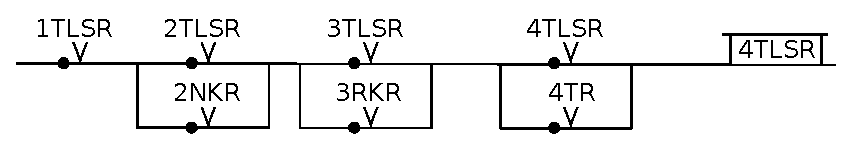
\includegraphics[keepaspectratio, width=100mm]{fig1.eps}
    \begin{displaymath}
      \text{\it TLSR}_{1T} \wedge (\text{\it TLSR}_{2T} \vee
      \text{\it NKR}_{\#2}) \wedge (\text{\it TLSR}_{3T} \vee
      \text{\it RKR}_{\#3}) \wedge (\text{\it TLSR}_{4T} \vee
      \text{\it TR}_{4}) : \mathcal{R}_{\text{\it TLSR}_{4T}}
    \end{displaymath}
    \begin{displaymath}
      \text{\it where}\;\; \mathcal{R}_{\text{\it TLSR}_{4T}} =
      \bigl(\text{\it TLSR} \vee
      {(\text{\it NKR} | \text{\it RKR})}^? \bigr)^* \wedge
      (\text{\it TLSR} \vee \text{\it TR})
    \end{displaymath}
    \caption{polymorphic matching of interlocking logic example 1}
    \label{fig_of_polymatching_ex1}
  \end{center}
\end{figure}


We can express above instance as
\verb@TLSR_1T & (TLSR_2T | NKR_#2) & (TLSR_3T@
\verb@ | RKR_#3) & (TLSR_4T | TR_4)@, accroding to def. of term,
and pattern is also expressed
as \verb@(TLSR | (NKR % RKR)?)* & (TLSR | TR)@.
Consequently, we are trying patternmatching, and the result of it is
shown as follows.
\begin{verbatim}
# term (typematch (compile "TLSR_1T & (TLSR_2T | NKR_#2) & (TLS
R_3T | RKR_#3) & (TLSR_4T | TR_4) : (TLSR | (NKR % RKR)?)* & (T
LSR | TR)"));;
- : "(TLSR_1T & ((((TLSR_2T | NKR_#2)) & ((((TLSR_3T | RKR_#3))
 & ((TLSR_4T | TR_4)))))))"
\end{verbatim}

Looking at the last line of above, it just been generated from her
coginition, which shows that LIezA has successed to match given term with
pattern, and recognized its structual meaning, which has been stored as
the form of Binding internally. We can still access more specific ones on
her cognition as follows.
\begin{verbatim}
# let sr_trg = cli_pat (compile "* : (TLSR | (NKR % RKR)?)*");;
val sig_trg : Lie_type.pattern = ...
# foreach (resolv sr_trg (typematch (compile "TLSR_1T & (TLSR_2
T | NKR_#2) & (TLSR_3T | RKR_#3) & (TLSR_4T | TR_4) : (TLSR | (
NKR % RKR)?)* & (TLSR | TR)")));;
- : string list = ["(((TLSR_1T | *)) & ((((TLSR_2T | NKR_#2)) &
 ((TLSR_3T | RKR_#3)))))"]
\end{verbatim}

The first command of above specifies the target pattern we refer.
Then we try to refer the subterms bound to the target
pattern, which is currently assigned to \verb|sr_trg|, on next command,
And we can find that the last line depicts the subterm bound to the target
pattern we specified correctly.

Similar to above, we can access other internal subterms in her again.
\begin{verbatim}
# let sr_rel = cli_pat (compile "* : (TLSR | TR)");;
val sig_ctrl : Lie_type.pattern = ...
# foreach (resolv sr_rel (typematch (compile "TLSR_1T & (TLSR_2
T | NKR_#2) & (TLSR_3T | RKR_#3) & (TLSR_4T | TR_4) : (TLSR | (
NKR % RKR)?)* & (TLSR | TR)")));;
- : string list = ["(TLSR_4T | TR_4)"]
\end{verbatim}

Finally, we present more practical examples in the domain of railway
signaling engineering.

We suppose the following entity of interlocking logic, which is called as
Signal Controlling Circuit,
\begin{figure}[htbp]
  \begin{center}
    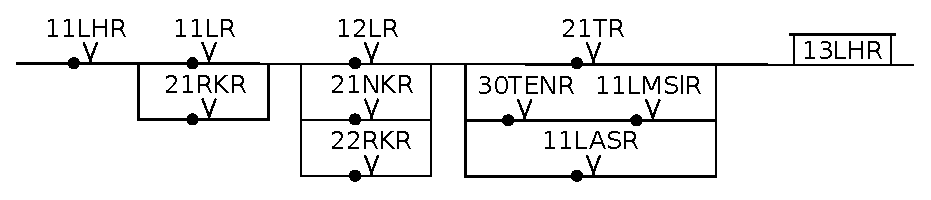
\includegraphics[keepaspectratio, width=100mm]{fig_HR.eps}
    \caption{interlocking logic example 2, Signal Control Circult}
    \label{fig_of_instance_ex1}
  \end{center}
\end{figure}

and we also know which can be expressed generally as
$\text{\it HR} \wedge \bigl(\text{\it LR} \vee
(\text{\it NKR} | \text{\it RKR})^\downarrow \bigr)^* \wedge
\bigl(\text{\it TR}^+ \vee (\text{\it TENR} \wedge \text{\it MSlR}) \vee
\text{\it ASR} \bigr)$.

We express above circuit as
\verb@HR_11L&(LR_11|RKR_#21)&(LR_12|NKR_#21|RKR_#22)@
\verb@&(TR_21i|(TENR_30&MSlR_11L)|ASR_11L)@, and try to feed LIezA them as
follow.
\begin{verbatim}
# term (typematch (compile "HR_11L & (LR_11 | RKR_#21) & (LR_12 |
NKR_#21 | RKR_#22) & (TR_21i | (TENR_30 & MSlR_11L) | ASR_11L) :
HR & (LR | (NKR % RKR)!)* & (TR+ | (TENR & MSlR) | ASR)"));;
- : string ="(HR_11L & ((((LR_11 | RKR_#21)) & ((((LR_12 |
((NKR_#21 | RKR_#22)))) & ((TR_21i | ((((TENR_30 & MSlR_11L)) |
ASR_11L)))))))))"
\end{verbatim}

Then we make confirm her cognition for specific conditions on this circuit.
Our pattern for Signal Controlling Circuit has a $\text{\it ASR}$ as
its subpattern, which corresponds to verification of Approaching Stick
Locking a.k.a. ASR on related route's signal aspect controlling.
And we can see the condition of ASR verification by searching the one
bound to the subpattern of $\text{\it ASR}$, as follow.
\begin{verbatim}
# let ver_ASR = cli_pat (compile "* : ASR");;
val ver_ASR : Lie_type.pattern = ...
# foreach (resolv ver_ASR (typematch (compile "HR_11L & (LR_11 |
RKR_21) & (LR_12 | NKR_#21 | RKR_#22) & (TR_21i | (TENR_30 &
MSlR_11L) | ASR_11L) : HR & (LR | (NKR % RKR)!)* & (TR+ | (TENR &
MSlR) | ASR)")));;
- : string list = ["ASR_11L"]
\end{verbatim}
LIezA correctly recognized and replied the condition we queried on
the last line, as desired.

Similarly we try again to refer the condition of Approaching Track, which is
another specific one occuring on Signal Controlling Circuit . And we also
obtain correct result from LIezA, as follow.
\begin{verbatim}
# let ver_appTR = cli_pat (compile "* : TR+");;
val ver_appTR : Lie_type.pattern = ...
# foreach (resolv ver_appTR (typematch (compile "HR_11L & (LR_11 |
RKR_21) & (LR_12 | NKR_#21 | RKR_#22) & (TR_21i | (TENR_30 &
MSlR_11L) | ASR_11L) : HR & (LR | (NKR % RKR)!)* & (TR+ | (TENR &
MSlR) | ASR)")));;
- : string list = ["TR_21i"]
\end{verbatim}


\pagebreak
\section{Appendix 1: supplementary proofs}
\label{Appendix_1}

\begin{Definition}
  \[ \mathpzc{Gnd}(\Delta) \;\stackrel{\mathrm{def}}{:=}
      \bigl\{t_{\text{\it equ}}\ |\ (t, t_{\text{\it equ}}, \mathcal{R},
       \mathcal{S}_{\mathpzc{fin}}, \Delta') \in \Delta\ \text{\it s.t.}\
        \mathcal{S}_{\mathpzc{fin}} \in \{\text{\it gnd}, \text{\it def},
         \text{\it nil} \} \bigr\}
  \]
\end{Definition}


\begin{Property}
  \label{consistency_on_grand_terms}
  \[ \mathpzc{gnd}\Bigl(\mathcal{M}\bigl(\Delta(t) \bigr) \Bigr) =
      \mathpzc{Gnd}(\Delta)\ \text{\it s.t.}\
       \Delta \vdash t \triangleright \mathcal{R}
  \]
  \begin{Proof}
    Proof is simple induction on derivation for
    $\Delta \vdash t \triangleright \mathcal{R}$.
    $\Box$
  \end{Proof}
\end{Property}


\begin{Property}
  \label{consistency_on_domain_independency}
  \[ \begin{array}{r}
       \mathpzc{Dom}(\Delta_1) \cap \mathpzc{Dom}(\Delta_2) = \phi\
        \text{\it where}\ \Delta_1 \vdash t_1 \triangleright \mathcal{R}_1\
         \text{\it and}\ \Delta_2 \vdash t_2 \triangleright \mathcal{R}_2,\
          \text{\it then}  \\
       \mathpzc{sub}\Bigl(\mathcal{M}\bigl(\Delta_1(t_1) \bigr) \Bigr) \cap
        \mathpzc{sub}\Bigl(\mathcal{M}\bigl(\Delta_2(t_2) \bigr) \Bigr) = \phi
     \end{array}
  \]
  \begin{Proof}
    From def. of $\mathpzc{sub}$ and $\mathcal{M}$, any term in
    $\mathpzc{sub}\Bigl(\mathcal{M}\bigl(\Delta_1(t_1) \bigr) \Bigr)$
    consists of the grand terms belonging to
    $\mathpzc{gnd}\Bigl(\mathcal{M}\bigl(\Delta_1(t_1) \bigr) \Bigr)$, i.e.
    all of grand terms occuring on
    $t \in \mathpzc{sub}\Bigl(\mathcal{M}\bigl(\Delta_1(t_1) \bigr) \Bigr)$
    is comming from
    $\mathpzc{gnd}\Bigl(\mathcal{M}\bigl(\Delta_1(t_1) \bigr) \Bigr)$.
    $\mathpzc{sub}\Bigl(\mathcal{M}\bigl(\Delta_2(t_2) \bigr) \Bigr)$ is
    Similar. Consequently accounting on the facts of
    $\mathpzc{gnd}\Bigl(\mathcal{M}\bigl(\Delta_1(t_1) \bigr) \Bigr) =
    \mathpzc{Gnd}(\Delta_1) \subseteq \mathpzc{Dom}(\Delta_1)$ and
    $\mathpzc{gnd}\Bigl(\mathcal{M}\bigl(\Delta_1(t_2) \bigr) \Bigr) =
    \mathpzc{Gnd}(\Delta_2) \subseteq \mathpzc{Dom}(\Delta_2)$ from
    Property \ref{consistency_on_grand_terms} respectively. Thus we find that
    $\mathpzc{gnd}\Bigl(\mathcal{M}\bigl(\Delta_1(t_1) \bigr) \Bigr) \cap
    \mathpzc{gnd}\Bigl(\mathcal{M}\bigl(\Delta_2(t_2) \bigr) \Bigr) = \phi$
    for $\mathpzc{Dom}(\Delta_1) \cap \mathpzc{Dom}(\Delta_2) = \phi$, which
    implies
    $\mathpzc{sub}\Bigl(\mathcal{M}\bigl(\Delta_1(t_1) \bigr) \Bigr) \cap
    \mathpzc{sub}\Bigl(\mathcal{M}\bigl(\Delta_2(t_2) \bigr) \Bigr) = \phi$.
    $\Box$
  \end{Proof}
\end{Property}


\begin{Lemma}{completeness on extended matching.}
  \label{completeness_on_extended_matching}
  \[ \Gamma \vdash \mathcal{M}\bigl( \Delta(t) \bigr) : \mathcal{R}\;\;
      \text{\it for some}\ \Gamma,\ \text{\it where}\
       \Delta \vdash t \triangleright \mathcal{R}.
  \]
  \begin{Proof}
    Proof is induction on structure of derivation of
    $\Gamma \vdash t \triangleright \mathcal{R}$.
    
    Case (T-Atom0-xtend): From def. of (T-Atom0-xtend), we suppose
    $\bigl\{(t, t_0, \mathcal{R}_0, \text{\it gnd}, \phi) \bigr\} \vdash
    t \triangleright \mathcal{R}_0$ s.t. $t \simeq t_0$ with
    $(t_0, \mathcal{R}_0) \in \Gamma_\text{\it gnd}$. Then
    we can derive $\bigl\{(t_0, \mathcal{R}_0) \bigr\} \vdash
    \mathcal{M}\bigl(\Delta(t) \bigr): \mathcal{R}_0$
    from (T-Atom0-canon), since
    $\mathcal{M}\bigl(\Delta(t) \bigr) = \mathcal{M}(t, t_0, \mathcal{R}_0,
    \text{\it gnd}, \phi) = t_0$ from def of $\mathcal{M}$.
    
    Case (T-Atom1-xtend): Proof is same as the case of (T-Atom0-xtend).
    
    Case (T-Cas-xtend): In this case, we suppose that
    $\Delta \vdash t \triangleright \mathcal{R}_1 \wedge \mathcal{R}_2$
    where we let
    $\Delta = \Bigl\{\bigl(t, t_1 \wedge t_2,
    \mathcal{R}_1 \wedge \mathcal{R}_2, \wedge, (\Delta_1 \cup \Delta_2)
    \bigr) \Bigr\} \cup (\Delta_1 \cup \Delta_2)$ for some $\Delta_1$ and
    $\Delta_2$ satisfying
    $\Delta_1 \vdash t_1 \triangleright \mathcal{R}_1$,
    $\Delta_2 \vdash t_2 \triangleright \mathcal{R}_2$ and
    $\mathpzc{Dom}(\Delta_1) \cap \mathpzc{Dom}(\Delta_2) = \phi$ from
    def. of (T-Cas-xtend). By induction hypothesis, we suppose that
    $\Gamma_1 \vdash \mathcal{M}\bigl(\Delta_1(t_1) \bigr) : \mathcal{R}_1$
    and
    $\Gamma_2 \vdash \mathcal{M}\bigl(\Delta_2(t_2) \bigr) : \mathcal{R}_2$
    for some $\Gamma_1$ and $\Gamma_2$ where
    $\Delta_1(t_1) = (t_1, t_{\text{\it equ}_1}, \mathcal{R}_1,
    \mathcal{S}_1, \Delta_1')$ and
    $\Delta_2(t_2) = (t_2, t_{\text{\it equ}_2}, \mathcal{R}_2,
    \mathcal{S}_2, \Delta_2')$ respectively.
    According to the facts that
    $\mathpzc{Dom}(\Delta_1 \cup \Delta_2) =
    \mathpzc{Dom}(\Delta_1) \cup \mathpzc{Dom}(\Delta_2)$ s.t.
    $\mathpzc{Dom}(\Delta_1) \cap \mathpzc{Dom}(\Delta_2) = \phi$, we find
    $t_1 \not\in \mathpzc{Dom}(\Delta_2)$ s.t.
    $t_1 \in \mathpzc{Dom}(\Delta_1)$ for
    $\Delta_1 \vdash t_1 \triangleright \mathcal{R}_1$, and
    $t_2 \not\in \mathpzc{Dom}(\Delta_1)$ s.t
    $t_2 \in \mathpzc{Dom}(\Delta_2)$ for
    $\Delta_2 \vdash t_2 \triangleright \mathcal{R}_2$. Thus
    $\mathcal{M}\bigl(\Delta(t) \bigr) =
    \mathcal{M}\bigl(t, t_1 \wedge t_2, \mathcal{R}_1 \wedge \mathcal{R}_2,
    \wedge, (\Delta_1 \cup \Delta_2) \bigr) =
    \mathcal{M}\bigl((\Delta_1 \cup \Delta_2)(t_1) \bigr) \wedge
    \mathcal{M}\bigl((\Delta_1 \cup \Delta_2)(t_2) \bigr) =
    \mathcal{M}\bigl(\Delta_1(t_1) \bigr) \wedge \mathcal{M}\bigl(
    \Delta_2(t_2) \bigr)$ allows us to conclude
    $\biggl\{\Bigl(\mathcal{M}\bigl(\Delta_1(t_1) \bigr) \wedge
    \mathcal{M}\bigl(\Delta_2(t_2) \bigr), \mathcal{R}_1 \wedge
    \mathcal{R}_2 \Bigr) \biggr\} \cup (\Gamma_1 \cup \Gamma_2) \vdash
    \mathcal{M}\bigl(\Delta_1(t_1) \bigr) \wedge \mathcal{M}\bigl(
    \Delta_2(t_2) \bigr) : \mathcal{R}_1 \wedge \mathcal{R}_2$ from
    (T-Cas-canon), with the conditions of
    $\mathpzc{Dom}(\Gamma_1) \cap \mathpzc{Dom}(\Gamma_2) = \phi$ and
    $\mathcal{M}\bigl(\Delta_1(t_1) \bigr) \wedge \mathcal{M}\bigl(
    \Delta_2(t_2) \bigr) \not\in \mathpzc{Dom}(\Gamma_1 \cup \Gamma_2)$ as
    follows. We find that
    $\mathpzc{sub}\Bigl(\mathcal{M}\bigl(\Delta_1(t_1) \bigr) \Bigr) \cap
    \mathpzc{sub}\Bigl(\mathcal{M}\bigl(\Delta_2(t_2) \bigr) \Bigr) = \phi$
    from the facts of
    $\mathpzc{Dom}(\Delta_1) \cap \mathpzc{Dom}(\Delta_2) = \phi$ s.t.
    $\Delta_1 \vdash t_1 \triangleright \mathcal{R}_1$ and
    $\Delta_2 \vdash t_2 \triangleright \mathcal{R}_2$ with
    Property \ref{consistency_on_domain_independency}, then we even do
    $\mathpzc{Dom}(\Gamma_1) \subseteq \mathpzc{sub}\Bigl(\mathcal{M}\bigl(
    \Delta_1(t_1) \bigr) \Bigr)$ and
    $\mathpzc{Dom}(\Gamma_2) \subseteq \mathpzc{sub}\Bigl(\mathcal{M}\bigl(
    \Delta_2(t_2) \bigr) \Bigr)$ where
    $\Gamma_1 \vdash \mathcal{M}\bigl(\Delta_1(t_1) \bigr) :
    \mathcal{R}_1$ and
    $\Gamma_2 \vdash \mathcal{M}\bigl(\Delta_2(t_2) \bigr) :
    \mathcal{R}_2$ respectively from Property \ref{dom_of_Gamma}, thus
    $\mathpzc{Dom}(\Gamma_1) \cap \mathpzc{Dom}(\Gamma_2) = \phi$.
    Consequently, we show the reason of
    $\mathcal{M}\bigl(\Delta_1(t_1) \bigr) \wedge
    \mathcal{M}\bigl(\Delta_2(t_2) \bigr) \not\in 
    \mathpzc{Dom}(\Gamma_1 \cup \Gamma_2)$. We know that
    $\mathpzc{size}\Bigl(\mathcal{M}\bigl(\Delta_1(t_1) \bigr) \wedge
    \mathcal{M}\bigl(\Delta_2(t_2) \bigr) \Bigr) >
    \mathpzc{size}\Bigl(\mathcal{M}\bigl(\Delta_1(t_1) \bigr) \Bigr) \ge
    \mathpzc{size}(t'_1)$ for any $t'_1 \in \mathpzc{Dom}(\Gamma_1)$
    from Property \ref{termsize_constraint_on_Gamma}, which implies that
    $\mathcal{M}\bigl(\Delta_1(t_1) \bigr) \wedge
    \mathcal{M}\bigl(\Delta_2(t_2) \bigr) \not\in \mathpzc{Dom}(\Gamma_1)$
    and $\mathcal{M}\bigl(\Delta_1(t_1) \bigr) \wedge
    \mathcal{M}\bigl(\Delta_2(t_2) \bigr) \not\in \mathpzc{Dom}(\Gamma_2)$
    respectively, thus we obtain
    $\mathcal{M}\bigl(\Delta_1(t_1) \bigr) \wedge
    \mathcal{M}\bigl(\Delta_2(t_2) \bigr) \not\in
    \Bigl(\mathpzc{Dom}(\Gamma_1) \cup \mathpzc{Dom}(\Gamma_2) \Bigr) =
    \mathpzc{Dom}(\Gamma_1 \cup \Gamma_2)$. Note that we call the
    reason of above, i.e.
    $\mathcal{M}\bigl(\Delta_1(t_1) \bigr) \wedge
    \mathcal{M}\bigl(\Delta_2(t_2) \bigr) \not\in
    \mathpzc{Dom}(\Gamma_1 \cup \Gamma_2)$, as ``term size constraint''
    in below argument.
    
    Case (T-Par-xtend): Proof is same as the case of (T-Cas-xtend).
    
    Case (T-Cat0-xtend-nil): Similar to the case of (T-Atom0-xtend) as
    follow. We suppose
    $\Bigl\{\bigl(t, \{\}, {\mathcal{R}_1}^*, \text{\it nil}, \phi \bigr)
    \Bigr\} \vdash t \triangleright {\mathcal{R}_1}^*$ s.t.
    $t \simeq \{\}$. Thus we can derive
    $\Bigl\{\bigl(\{\}, {\mathcal{R}_1}^* \bigr) \Bigr\} \vdash
    \mathcal{M}\bigl(\Delta(t) \bigr): {\mathcal{R}_0}^*$ from
    (T-Cat0-canon-nil), since
    $\mathcal{M}\bigl(\Delta(t) \bigr) =
    \mathcal{M}\bigl(t, \{\}, {\mathcal{R}_0}^*, \text{\it nil}, \phi
    \bigr) = \{\}$ from def of $\mathcal{M}$.
    
    Case (T-Cat0-xtend-sol): In this case, we suppose the deduction of
    $\Delta \vdash t \triangleright {\mathcal{R}_1}^*$ from
    (T-Cat0-xtend-sol) where we let
    $\Delta = \bigl\{(t, t', {\mathcal{R}_1}^*, \text{\it sol}, \Delta')
    \bigr\} \cup \Delta'$, which also implies the existence of
    derivation of $\Delta' \vdash t' \triangleright \mathcal{R}_1$ s.t.
    $t \simeq t'$ and $t \not\in \mathpzc{Dom}(\Delta')$. for some
    $\Delta'$. According to the fact that
    $\Gamma' \vdash \mathcal{M}\bigl(\Delta'(t') \bigr) : \mathcal{R}_1$
    for some $\Gamma'$ obtained by applying induction hypothesis on
    $\Delta' \vdash t' \triangleright \mathcal{R}_1$, we have
    $\Biggl\{\biggl(\Bigl\{\mathcal{M}\bigl(\Delta'(t') \bigr) \Bigr\},
    {\mathcal{R}_1}^* \biggr) \Biggr\} \cup \Gamma' \vdash \Bigl\{
    \mathcal{M}\bigl(\Delta'(t') \bigr) \Bigr\} : {\mathcal{R}_1}^*$ from
    (T-Cat0-canon-$\infty$), since
    $\mathcal{M}\bigl(\Delta(t) \bigr) =
    \mathcal{M}(t, t', {\mathcal{R}_1}^*, \text{\it sol}, \Delta') =
    \Bigl\{\mathcal{M}\bigl(\Delta'(t') \bigr) \Bigr\}$ s.t
    $\Bigl\{\mathcal{M}\bigl(\Delta'(t') \bigr) \Bigr\} \not\in
    \mathpzc{Dom}(\Gamma')$ by term size constraint.
    
    Case (T-Cat0-xtend-$\infty$): In this case, we suppose the last applied
    on deduction of $\Delta \vdash t \triangleright {\mathcal{R}_1}^*$ is
    (T-Cat0-xtend-$\infty$), where we let
    $\Delta = \Bigl\{\bigl(t, t_h \wedge t'_t, {\mathcal{R}_1}^*, \infty,
    (\Delta_h \cup \Delta'_t) \bigr) \Bigr\} \cup (\Delta_h \cup \Delta'_t)$
    s.t. $\Delta_h = \bigl\{(t_h, t'_h, \mathcal{R}_1, \mathcal{S}_h,
    \Delta'_h)\bigr\} \cup \Delta'_h$ and
    $\Delta_t = \bigl\{(t_t, t'_t, {\mathcal{R}_1}^*, \mathcal{S}_t,
    \Delta'_t) \bigr\} \cup \Delta'_t$ comming from
    $\Delta_h \vdash t_h \triangleright \mathcal{R}_1$ and
    $\Delta_t \vdash t_t \triangleright {\mathcal{R}_1}^*$ as respective.
    Additionally, there are 2 cases to be considered, focusing on
    the derivation of $\Delta_t \vdash t_t \triangleright {\mathcal{R}_1}^*$
    as follows.
    Subcase (T-Cat0-xtend-sol): In this case, we suppose that
    the last applied rule on the derivation of
    $\Delta_t \vdash t_t \triangleright {\mathcal{R}_1}^*$ is
    (T-Cat0-xtend-sol), where
    $\Delta_t = \bigl\{(t_t, t'_t, {\mathcal{R}_1}^*, \text{\it sol},
    \Delta'_t) \bigr\} \cup \Delta'_t$ and
    $\Delta'_t = (t'_t, t''_t, \mathcal{R}_1, \mathcal{S}_{t'},
    \Delta''_t)$ s.t. $\Delta'_t \vdash t'_t \triangleright \mathcal{R}_1$
    we let. By applying induction hypothesis on
    $\Delta_h \vdash t_h \triangleright \mathcal{R}_1$, we find
    $\Gamma_h \vdash \mathcal{M}\bigl(\Delta_h(t_h) \bigr) : \mathcal{R}_1$
    for some $\Gamma_h$. Similarly, we can also obtain
    $\Gamma'_t \vdash \mathcal{M}\bigl(\Delta'_t(t'_t) \bigr) :
    \mathcal{R}_1$ for some $\Gamma'_t$ from induction hypothesis for
    $\Delta'_t \vdash t'_t \triangleright \mathcal{R}_1$.
    Accounting on the fact that
    $\mathpzc{Dom}(\Delta'_t) \subseteq \mathpzc{Dom}(\Delta_t)$ where
    $\Delta_t = \bigl\{(t_t, t'_t, {\mathcal{R}_1}^*, \text{\it sol},
    \Delta'_t) \bigr\} \cup \Delta'_t$, we find
    $\mathpzc{Dom}(\Delta_h) \cap \mathpzc{Dom}(\Delta'_t) = \phi$, because
    of $\mathpzc{Dom}(\Delta_h) \cap \mathpzc{Dom}(\Delta_t) = \phi$ from
    the def. of (T-Cat0-xtend-$\infty$). Then we can say that
    $\mathpzc{sub}\Bigl(\mathcal{M}\bigl(\Delta_h(t_h) \bigr) \Bigr) \cap
    \mathpzc{sub}\Bigl(\mathcal{M}\bigl(\Delta'_t(t'_t) \bigr) \Bigr) =
    \phi$ from Lemma \ref{consistency_on_domain_independency} for
    $\Delta_h \vdash t_h \triangleright \mathcal{R}_1$ and
    $\Delta'_t \vdash t'_t \triangleright \mathcal{R}_1$ above. By now,
    recalling the facts we revealed above as
    $\Gamma_h \vdash \mathcal{M}\bigl(\Delta_h(t_h) \bigr) : \mathcal{R}_1$
    and $\Gamma'_t \vdash \mathcal{M}\bigl(\Delta'_t(t'_t) \bigr) :
    \mathcal{R}_1$ for some $\Gamma_h$ and $\Gamma'_t$ respectively, we
    still find that
    $\mathpzc{Dom}(\Gamma_h) \subseteq \mathpzc{sub}\Bigl(\mathcal{M}\bigl(
    \Delta_h(t_h) \bigr) \Bigr)$ and
    $\mathpzc{Dom}(\Gamma'_t) \subseteq \mathpzc{sub}\Bigl(\mathcal{M}\bigl(
    \Delta'_t(t'_t) \bigr) \Bigr)$ from
    Property \ref{dom_of_Gamma}, thus we find
    $\mathpzc{Dom}(\Gamma_h) \cap \mathpzc{Dom}(\Gamma'_t) = \phi$.
    Accordingly we obtain the conclusion that
    $\biggl\{\Bigl(\bigl\{\mathcal{M}\bigl(\Delta_h(t_h) \bigr),
    \mathcal{M}\bigl(\Delta'_t(t'_t) \bigr) \bigr\}, {\mathcal{R}_1}^*
    \Bigr) \biggr\} \cup (\Gamma_h \cup \Gamma'_t) \vdash
    \Bigl\{\mathcal{M}\bigl(\Delta_h(t_h) \bigr), \mathcal{M}\bigl(
    \Delta'_t(t'_t) \bigr) \Bigr\} : {\mathcal{R}_1}^*$ from
    (T-Cat0-canon-$\infty$), where we mention that
    $\mathcal{M}\bigl(\Delta(t) \bigr) =
    \mathcal{M}\bigl(t, t_h \wedge t'_t, {\mathcal{R}_1}^*, \infty,
    (\Delta_h \cup \Delta'_t) \bigr) =
    \Bigl\{\mathcal{M}\bigl((\Delta_h \cup \Delta'_t)(t_h) \bigr),
    \mathcal{M}\bigl((\Delta_h \cup \Delta'_t)(t'_t) \bigr) \Bigr\} =
    \Bigl\{\mathcal{M}\bigl(\Delta_h(t_h) \bigr),
    \mathcal{M}\bigl(\Delta'_t(t'_t) \bigr) \Bigr\}$ since
    $(\Delta_h \cup \Delta'_t)(t_h) = \Delta_h(t_h)$ and
    $(\Delta_h \cup \Delta'_t)(t'_t) = \Delta'_t(t'_t)$ from the fact of
    $\mathpzc{Dom}(\Delta_h) \cap \mathpzc{Dom}(\Delta'_t) = \phi$ as above,
    thus $\Bigl\{\mathcal{M}\bigl(\Delta_h(t_h) \bigr), \mathcal{M}\bigl(
    \Delta'_t(t'_t) \bigr) \Bigr\} \not\in \mathpzc{Dom}(\Gamma_h)$ and
    $\Bigl\{\mathcal{M}\bigl(\Delta_h(t_h) \bigr), \mathcal{M}\bigl(
    \Delta'_t(t'_t) \bigr) \Bigr\} \not\in \mathpzc{Dom}(\Gamma'_t)$ s.t.
    $\Gamma_h \vdash \mathcal{M}\bigl(\Delta_h(t_h) \bigr) : \mathcal{R}_1$
    and $\Gamma'_t \vdash \mathcal{M}\bigl(\Delta'_t(t'_t) \bigr) :
    \mathcal{R}_1$ respectively by term size constraint. i.e.
    $\mathpzc{size}\biggl(\Bigl\{\mathcal{M}\bigl(\Delta_h(t_h) \bigr),
    \mathcal{M}\bigl(\Delta'_t(t'_t) \bigr) \Bigr\} \biggr) >
    \mathpzc{size}\Bigl(\mathcal{M}\bigl(\Delta_h(t_h) \bigr) \Bigr) \ge
    \mathpzc{size}(t')$ for any $t' \in \mathpzc{Dom}(\Gamma_h)$ s.t.
    $\Gamma_h \vdash \mathcal{M}\bigl(\Delta_h(t_h) \bigr) : \mathcal{R}_1$, 
    which implies
    $\Bigl\{\mathcal{M}\bigl(\Delta_h(t_h) \bigr), \mathcal{M}\bigl(
    \Delta'_t(t'_t) \bigr) \Bigr\} \not\in \mathpzc{Dom}(\Gamma_h)$,
    $\Bigl\{\mathcal{M}\bigl(\Delta_h(t_h) \bigr), \mathcal{M}\bigl(
    \Delta'_t(t'_t) \bigr) \Bigr\} \not\in \mathpzc{Dom}(\Gamma'_t)$ is
    similar. Therefore
    $\bigl\{\mathcal{M}\bigl(\Delta_h(t_h) \bigr), \mathcal{M}\bigl(
    \Delta'_t(t'_t) \bigr) \bigr\} \not\in
    \bigl(\mathpzc{Dom}(\Gamma_h) \cup \mathpzc{Dom}(\Gamma'_t) \bigr)$ as
    desired.
    Subcase (T-Cat0-xtend-$\infty$): Otherwise, i.e. in the case of that
    the last applied rule on
    $\Delta_t \vdash t_t \triangleright {\mathcal{R}_1}^*$ isn't
    (T-Cat0-xtend-sol), we can predicate that the last one applied on
    $\Delta_t \vdash t_t \triangleright {\mathcal{R}_1}^*$ is just
    (T-Cat0-xtend-$\infty$), since the constraint of $t'_t \neq \{\}$ on
    $\Delta_t(t_t) = (t_t, t'_t, {\mathcal{R}_1}^*, \mathcal{S}_{t},
    \Delta'_t)$ eliminates the case of (T-Cat0-xtend-nil) as the last
    applied rule. Accordingly we suppose
    $\Delta_t = \bigl\{(t_t, t'_t, {\mathcal{R}_1}^*, \infty, \Delta'_t)
    \bigr\} \cup \Delta'_t$ s.t.
    $t'_t = t_{t_h} \wedge t'_{t_t}$ and
    $\Delta'_t = \Delta_{t_h} \cup \Delta'_{t_t}$, where we let
    $\Delta_{t_h} = \bigl\{(t_{t_h}, t'_{t_h}, \mathcal{R}_1,
    \mathcal{S}_{t_h}, \Delta'_{t_h} ) \bigr\} \cup \Delta'_{t_h}$, and
    $\Delta_{t_t} = \bigl\{(t_{t_t}, t'_{t_t}, {\mathcal{R}_1}^*,
    \mathcal{S}_{t_t}, \Delta'_{t_t} ) \bigr\} \cup \Delta'_{t_t}$ s.t.
    $\Delta_{t_h} \vdash t_{t_h} \triangleright \mathcal{R}_1$ and
    $\Delta_{t_t} \vdash t_{t_t} \triangleright {\mathcal{R}_1}^*$
    respectively comming from subderivations of
    $\Delta_t \vdash t_t \triangleright {\mathcal{R}_1}^*$ by
    (T-Cat0-xtend-$\infty$). Based on above assumptions with
    the fact $t'_t \not\in \mathpzc{Dom}(\Delta_h \cup \Delta'_t)$
    since $\mathpzc{Dom}(\Delta_h \cup \Delta'_t) = \bigl(
    \mathpzc{Dom}(\Delta_h) \cup \mathpzc{Dom}(\Delta'_t) \bigr) \subseteq
    \bigl(\mathpzc{Dom}(\Delta_h) \cup \mathpzc{Dom}(\Delta_t) \bigr) =
    \mathpzc{Dom}(\Delta_h \cup \Delta_t)$ s.t.
    $t'_t \not\in \mathpzc{Dom}(\Delta_h \cup \Delta_t)$ from def. of
    (T-Cat0-xtend-$\infty$), we get
    $\mathcal{M}\bigl(\Delta(t) \bigr) =
    \mathcal{M}(t, t_h \wedge t'_t, {\mathcal{R}_1}^*, \infty,
    \Delta_h \cup \Delta'_t ) =
    \Bigl\{\mathcal{M}\bigl((\Delta_h \cup \Delta'_t)(t_h) \bigr),
    t_2, \cdots t_n \Bigr\} =
    \Bigl\{\mathcal{M}\bigl(\Delta_h(t_h) \bigr), t_2, \cdots t_n \Bigr\}$
    satisfying $\{t_2, \cdots t_n\} =
    \mathcal{M}_{\{\}}\biggl(t'_t, {\mathcal{R}_1}^*,\Bigl(
    (\Delta_h \cup \Delta'_t) \setminus \bigl((\Delta_h \cup \Delta'_t)(t_h)
    \cup \Delta'_h \bigr) \Bigr) \biggr) =
    \mathcal{M}_{\{\}}\biggl(t'_t, {\mathcal{R}_1}^*,\Bigl(
    (\Delta_h \cup \Delta'_t) \setminus \bigl(\Delta_h(t_h) \cup \Delta'_h
    \bigr) \Bigr) \biggr) =
    \mathcal{M}_{\{\}}\Bigl(t'_t, {\mathcal{R}_1}^*,\bigl(
    (\Delta_h \cup \Delta'_t) \setminus \Delta_h \bigr) \Bigr) =
    \mathcal{M}_{\{\}}(t'_t, {\mathcal{R}_1}^*, \Delta'_t )$ where
    $(\Delta_h \cup \Delta'_t)(t_h) = \Delta_h(t_h) = 
    (t_h, t'_h, \mathcal{R}_1, \mathcal{S}_h, \Delta'_h)$ for
    $t_h \not\in \mathpzc{Dom}(\Delta'_t)$. Note that
    $\Delta_h \vdash t_h \triangleright \mathcal{R}_1$ implies
    $t_h \in \mathpzc{Dom}(\Delta_h)$, thus
    we can say $t_h \not\in \mathpzc{Dom}(\Delta'_t)$ for
    $\mathpzc{Dom}(\Delta'_t) \subseteq \mathpzc{Dom}(\Delta_t)$ s.t.
    $\mathpzc{Dom}(\Delta_h) \cap \mathpzc{Dom}(\Delta_t) = \phi$. From
    def. of (T-Cat0-xtend-$\infty$) applied on
    $\Delta_t \vdash t_t \triangleright {\mathcal{R}_1}^*$, we know that
    $t'_t = t_{t_h} \wedge t'_{t_t} \not\in
    \bigl(\mathpzc{Dom}(\Delta_{t_h}) \cup \mathpzc{Dom}(\Delta'_{t_t})
    \bigr) = \mathpzc{Dom}(\Delta'_t)$ since
    $\bigl(\mathpzc{Dom}(\Delta_{t_h}) \cup \mathpzc{Dom}(\Delta'_{t_t})
    \bigr) \subseteq \bigl(\mathpzc{Dom}(\Delta_{t_h}) \cup \mathpzc{Dom}(
    \Delta_{t_t}) \bigr) = \mathpzc{Dom}(\Delta_{t_h} \cup \Delta_{t_t})$,
    then we look for $\{t_2, \cdots t_n\} =
    \mathcal{M}_{\{\}}(t'_t, {\mathcal{R}_1}^*, \Delta'_t ) =
    \Bigl\{\mathcal{M}\bigl(\Delta'_t(t_{t_h}) \bigr), t'_2, \cdots t'_m
    \Bigr\} =
    \Bigl\{\mathcal{M}\bigl(\Delta_{t_h}(t_{t_h}) \bigr), t'_2, \cdots t'_m
    \Bigr\}$ where
    $\{t'_2, \cdots t'_m\} = \mathcal{M}_{\{\}}\biggl(
    t'_{t_t}, {\mathcal{R}_1}^*, \Bigr(\Delta'_t \setminus \bigl(
    \Delta'_t(t_{t_h}) \cup \Delta'_{t_h} \bigr) \Bigr) \biggr)$ s.t.
    $\Delta'_t(t_{t_h}) = (\Delta_{t_h} \cup \Delta'_{t_t})(t_{t_h}) =
    \Delta_{t_h}(t_{t_h}) =  (t_{t_h}, t'_{t_h}, \mathcal{R}_1,
    \mathcal{S}_{t_h}, \Delta'_{t_h} )$ since
    $t_{t_h} \not\in \mathpzc{Dom}(\Delta'_{t_t})$ for the same reason
    of $t_h \not\in \mathpzc{Dom}(\Delta'_t)$ as above. Then
    we can apply Claim \ref{claim1_for_completeness} on
    $\{t'_2, \cdots t'_m\} = \mathcal{M}_{\{\}}\biggl(
    t'_{t_t}, {\mathcal{R}_1}^*, \Bigr(\Delta'_t \setminus \bigl(
    \Delta'_t(t_{t_h}) \cup \Delta'_{t_h} \bigr) \Bigr) \biggr)$,
    we obtain the facts that
    $\Gamma'_2 \vdash t'_2: \mathcal{R}_1, \cdots
    \Gamma'_m \vdash t'_m: \mathcal{R}_1$ for some
    $\Gamma'_2, \cdots \Gamma'_m$ s.t.
    $\mathpzc{Dom}(\Gamma'_j) \cap \mathpzc{Dom}(\Gamma'_k) = \phi$ where
    $j \neq k$, and $\bigcup_{j=2}^m \mathpzc{Dom}(\Gamma'_j) \subseteq
    \mathpzc{sub}\Bigl(\mathcal{M}\bigl(\Delta_{t_t} (t_{t_t}) \bigr)
    \Bigr)$. According to the facts of
    $\mathpzc{Dom}(\Delta_{t_h}) \cap \mathpzc{Dom}(\Delta_{t_t}) = \phi$
    s.t. $\Delta_{t_h} \vdash t_{t_h} \triangleright \mathcal{R}_1$,
    $\Delta_{t_t} \vdash t_{t_t} \triangleright {\mathcal{R}_1}^*$, we get
    $\mathpzc{sub}\Bigl(\mathcal{M}\bigl(\Delta_{t_h}(t_{t_h}) \bigr)
    \Bigr) \cap \mathpzc{sub}\Bigl(\mathcal{M}\bigl(\Delta_{t_t}(t_{t_t})
    \bigr) \Bigr) = \phi$ with
    $\mathpzc{Dom}(\Gamma_{t_h}) \subseteq \mathpzc{sub}\Bigl(
    \mathcal{M}\bigl(\Delta_{t_h}(t_{t_h}) \bigr) \Bigr)$ s.t.
    $\Gamma_{t_h} \vdash \mathcal{M}\bigl(\Delta_{t_h}(t_{t_h}) \bigr) :
    \mathcal{R}_1$ from
    Property \ref{consistency_on_domain_independency}, \ref{dom_of_Gamma}
    and induction hypothesis applied on
    $\Delta_{t_h} \vdash t_{t_h} \triangleright \mathcal{R}_1$
    respectively. Thus we still find
    $\mathpzc{Dom}(\Gamma_{t_h}) \cap \bigcup_{j=2}^m\mathpzc{Dom}(
    \Gamma'_j) = \phi$ for
    $\bigcup_{j=2}^m\mathpzc{Dom}(\Gamma'_j) \subseteq \mathpzc{sub}\Bigl(
    \mathcal{M}\bigl(\Delta_{t_t}(t_{t_t}) \bigr) \Bigr)$ above.
    Accounting on the facts that
    $\mathpzc{Dom}(\Delta_{t_h}) \subseteq \mathpzc{Dom}(\Delta_t)$ s.t.
    $\mathpzc{Dom}(\Delta_h) \cap \mathpzc{Dom}(\Delta_t) = \phi$, which
    implies $\mathpzc{Dom}(\Delta_h) \cap \mathpzc{Dom}(\Delta_{t_h}) =
    \phi$, thus we find that
    $\mathpzc{sub}\Bigl(\mathcal{M}\bigl(\Delta_h(t_h) \bigr) \Bigr) \cap
    \mathpzc{sub}\Bigl(\mathcal{M}\bigl(\Delta_{t_h}(t_{t_h}) \bigr)
    \Bigr) = \phi$ similarly to above argument with
    Property \ref{consistency_on_domain_independency}. Since
    $\mathpzc{Dom}(\Gamma_h) \subseteq \mathpzc{sub}\Bigl(\mathcal{M}\bigl(
    \Delta_h(t_h) \bigr) \Bigr)$ s.t.
    $\Gamma_h \vdash \mathcal{M}\bigl(\Delta_h(t_h) \bigr) :
    \mathcal{R}_1$ and
    $\mathpzc{Dom}(\Gamma_{t_h}) \subseteq \mathpzc{sub}\Bigl(
    \mathcal{M}\bigl(\Delta_{t_h}(t_{t_h}) \bigr) \Bigr)$ s.t.
    $\Gamma_{t_h} \vdash \mathcal{M}\bigl(\Delta_{t_h}(t_{t_h}) \bigr) :
    \mathcal{R}_1$ both are from
    Property \ref{dom_of_Gamma}, then we obtain
    $\mathpzc{Dom}(\Gamma_{t_h}) \cap \bigl(\mathpzc{Dom}(\Gamma_h) \cup
    \bigcup_{j=2}^m \mathpzc{Dom}(\Gamma'_j) \bigr) = \phi$ for
    $\mathpzc{Dom}(\Gamma_{t_h}) \cap \bigcup_{j=2}^m \mathpzc{Dom}(
    \Gamma'_j) = \phi$ above. Similarly according to the facts of
    $\mathpzc{Dom}(\Delta_h) \cap \mathpzc{Dom}(\Delta_t) = \phi$ s.t.
    $\Delta_h \vdash t_h \triangleright \mathcal{R}_1$ and
    $\Delta_t \vdash t_t \triangleright {\mathcal{R}_1}^*$, we see that
    $\mathpzc{Dom}(\Gamma_h) \cap \mathpzc{Dom}(\Gamma_t) = \phi$ s.t
    $\Gamma_h \vdash \mathcal{M}\bigl(\Delta_h(t_h) \bigr) :
    \mathcal{R}_1$ and
    $\Gamma_t \vdash \mathcal{M}\bigl(\Delta_t(t_t) \bigr)
    :{\mathcal{R}_1}^*$ since
    $\mathpzc{sub}\Bigl(\mathcal{M}\bigl(\Delta_h(t_h) \bigr) \Bigr) \cap
    \mathpzc{sub}\Bigl(\mathcal{M}\bigl(\Delta_t(t_t) \bigr) \Bigr) =
    \phi$ s.t.
    $\mathpzc{Dom}(\Gamma_h) \subseteq
    \mathpzc{sub}\Bigl(\mathcal{M}\bigl(\Delta_h(t_h) \bigr) \Bigr)$ and
    $\mathpzc{Dom}(\Gamma_t) \subseteq
    \mathpzc{sub}\Bigl(\mathcal{M}\bigl(\Delta_t(t_t) \bigr) \Bigr)$ from
    Property \ref{consistency_on_domain_independency} and
    \ref{dom_of_Gamma} respectively.
    Next we focus on $\mathcal{M}\bigl(\Delta_t(t_t) \bigr)$ to show
    $\bigcup_{j=2}^m \mathpzc{Dom}(\Gamma'_j) \subseteq
    \mathpzc{sub}\Bigl(\mathcal{M}\bigl(\Delta_t(t_t) \bigr) \Bigr)$.
    From def of $\mathcal{M}$, we know that
    $\mathcal{M}\bigl(\Delta_t(t_t) \bigr) =
    \mathcal{M}(t_t, t'_t, {\mathcal{R}_1}^*, \infty, \Delta'_t) =
    \mathcal{M}(t_t, t_{t_h} \wedge t'_{t_t}, {\mathcal{R}_1}^*, \infty,
    \Delta'_t) =
    \Bigl\{\mathcal{M}\bigl(\Delta'_t(t_{t_h}) \bigr), t''_2, \cdots
    t''_l \Bigr\} =
    \Bigl\{\mathcal{M}\bigl((\Delta_{t_h} \cup \Delta'_{t_t})(t_{t_h})
    \bigr), t''_2, \cdots t''_l \Bigr\} =
    \Bigl\{\mathcal{M}\bigl(\Delta_{t_h}(t_{t_h}) \bigr), t''_2, \cdots
    t''_l \Bigr\}$ where
    $\{t''_2, \cdots t''_l \} =
    \mathcal{M}_{\{\}}\biggl(t'_{t_t}, {\mathcal{R}_1}^*, \Bigl(\Delta'_t
    \setminus \bigl(\Delta'_t(t_{t_h}) \cup \Delta'_{t_h} \bigr) \Bigr)
    \biggr) = \{t'_2, \cdots t'_m \}$ shown as above. Thus
    $\mathpzc{sub}\Bigl(\mathcal{M}\bigl(\Delta_t(t_t) \bigr) \Bigr) =
    \mathpzc{sub}\biggl(\Bigl\{\mathcal{M}\bigl(\Delta_{t_h}(t_{t_h}) \bigr),
    t'_2, \cdots t'_m \Bigr\} \biggr) \supseteq
    \bigcup_{j=2}^m \mathpzc{sub}(t'_j) \supseteq
    \bigcup_{j=2}^m \mathpzc{Dom}(\Gamma'_j)$ thus
    $\mathpzc{sub}\Bigl(\mathcal{M}\bigl(\Delta_t(t_t) \bigr) \Bigr)
    \supseteq \bigcup_{j=2}^m \mathpzc{Dom}(\Gamma'_j)$ s.t.
    $\Gamma'_j \vdash t'_j : \mathcal{R}_1$ for each $2 \le j \le m$.
    Therefore
    $\mathpzc{Dom}(\Gamma_h) \cap \bigcup_{j=2}^m \mathpzc{Dom}(\Gamma'_j)
    = \phi$ from
    $\mathpzc{sub}\Bigl(\mathcal{M}\bigl(\Delta_h(t_h) \bigr) \Bigr) \cap
    \mathpzc{sub}\Bigl(\mathcal{M}\bigl(\Delta_t(t_t) \bigr) \Bigr) =
    \phi$ with
    $\mathpzc{Dom}(\Gamma_h) \subseteq \mathpzc{sub}\Bigl(\mathcal{M}\bigl(
    \Delta_h(t_h) \bigr) \Bigr)$ revealed above, which even implies that
    $\mathpzc{Dom}(\Gamma_h) \cap \bigl(\mathpzc{Dom}(\Gamma_{t_h}) \cup
    \bigcup_{j=2}^m \mathpzc{Dom}(\Gamma'_j) \bigr) = \phi$ since
    $\mathpzc{Dom}(\Gamma_h) \cap \mathpzc{Dom}(\Gamma_{t_h}) = \phi$ as
    above. Consequently we have revealed that
    $\mathpzc{Dom}(\Gamma'_j) \cap \mathpzc{Dom}(\Gamma'_k) = \phi$ s.t.
    $j \neq k$,
    $\mathpzc{Dom}(\Gamma_{t_h}) \cap \bigcup_{j=2}^m \mathpzc{Dom}(
    \Gamma'_j) = \phi$ and
    $\mathpzc{Dom}(\Gamma_h) \cap \bigl(\mathpzc{Dom}(\Gamma_{t_h}) \cup
    \bigcup_{j=2}^m \mathpzc{Dom}(\Gamma'_j) \bigr) = \phi$, which
    allow us to conclude as
    $\biggl\{\Bigl(\mathcal{M}\bigl(\Delta(t) \bigr), {\mathcal{R}_1}^*
    \Bigr) \biggr\} \cup \bigl(\Gamma_h \cup \Gamma_{t_h} \cup
    \bigcup_{j=2}^m \Gamma'_j \bigr) \vdash
    \mathcal{M}\bigl(\Delta(t) \bigr) : {\mathcal{R}_1}^*$ where
    $\mathcal{M}\bigl(\Delta(t) \bigr) =
    \Bigl\{\mathcal{M}\bigl(\Delta_h(t_h) \bigr), t_2, \cdots t_n \Bigr\} =
    \Bigl\{\mathcal{M}\bigl(\Delta_h(t_h) \bigr),
    \mathcal{M}\bigl(\Delta_{t_h}(t_{t_h}) \bigr), t'_2, \cdots t'_m
    \Bigr\}$ s.t.
    $\Gamma_h \vdash \mathcal{M}\bigl(\Delta_h(t_h) \bigr) :
    \mathcal{R}_1$, for some $\Gamma_h$,
    $\Gamma_{t_h} \vdash \mathcal{M}\bigl(\Delta_{t_h}(t_{t_h}) \bigr) :
    \mathcal{R}_1$, for some $\Gamma_{t_h}$, and
    $\Gamma'_j \vdash t'_j : \mathcal{R}_1$ for each $2 \le j \le m$
    respectively. We mention that
    $\mathcal{M}\bigl(\Delta(t) \bigr) = \Bigl\{
    \mathcal{M}\bigl(\Delta_h(t_h) \bigr),
    \mathcal{M}\bigl(\Delta_{t_h}(t_{t_h}) \bigr), t'_2, \cdots t'_m
    \Bigr\} \not\in \mathpzc{Dom}\bigl(\Gamma_h \cup \Gamma_{t_h} \cup
    \bigcup_{j=2}^m \Gamma'_j \bigr)$ by size constraint, i.e.
    $\mathpzc{size}\Bigl(\mathcal{M}\bigl(\Delta(t) \bigr) \Bigr) >
    \mathpzc{size}\Bigl(\mathcal{M}\bigl(\Delta_h(t_h) \bigr) \Bigr)$,
    $\mathpzc{size}\Bigl(\mathcal{M}\bigl(\Delta_{t_h}(t_{t_h}) \bigr)
    \Bigr)$, $\mathpzc{size}(t'_2),\ \cdots \mathpzc{size}(t'_m)$, which
    implies $\mathcal{M}\bigl(\Delta(t) \bigr) \not\in \mathpzc{Dom}\bigl(
    \Gamma_h \cup \Gamma_{t_h} \cup \bigcup_{j=2}^m \Gamma'_j \bigr)$.
    
    Case (T-Cat1-xtend-sol):
    Proof is similar to the case of (T-Cat0-xtend-sol).
    
    Case (T-Cat1-xtend-$\infty$):
    Proof is similar to the case of (T-Cat0-xtend-$\infty$).
    
    Case (T-Dup-xtend-sol):
    Proof is similar to the case of case (T-Cat1-xtend-sol).
    
    Case (T-Dup-xtend-$\infty$):
    Proof is similar to the case of (T-Cat1-xtend-$\infty$).
    
    Case (T-Opt-xtend-nil):
    Proof is similar to the case of (T-Cat0-xtend-nil), from the def of
    $\mathcal{M}$ as
    $\mathcal{M}\bigl(\Delta(t) \bigr) =
    \mathcal{M}(t, \circ, {\mathcal{R}_1}^?, \text{\it nil}, \phi) =
    \circ$, with (T-Opt-canon-nil).

    Case (T-Opt-xtend-sol):
    We suppose
    $\Delta \vdash t \triangleright {\mathcal{R}_1}^?$ where we let
    $\Delta = \bigl\{(t, t', {\mathcal{R}_1}^?, \text{\it sol}, \Delta')
    \bigr\} \cup \Delta'$ s.t
    $\Delta' \vdash t' \triangleright \mathcal{R}_1$ from def. of
    (T-Opt-xtend-sol). Then from def. of $\mathcal{M}$, we obtain
    $\mathcal{M}\bigl(\Delta(t) \bigr) =
    \mathcal{M}(t, t', {\mathcal{R}_1}^?, \text{\it sol}, \Delta') =
    {\mathcal{M}\bigl(\Delta'(t') \bigr)}^?$ s.t.
    $\Gamma' \vdash \mathcal{M}\bigl(\Delta'(t') \bigr) : \mathcal{R}_1$
    for some $\Gamma'$ by induction hypothesis appled on
    $\Delta' \vdash t' \triangleright \mathcal{R}_1$, which also satisfies
    the condition that
    ${\mathcal{M}\bigl(\Delta'(t') \bigr)}^? \not\in \mathpzc{Dom}(
    \Gamma')$ by term size constraint. Thus we obtain
    $\biggl\{\Bigl({\mathcal{M}\bigl(\Delta'(t') \bigr)}^?,
    {\mathcal{R}_1}^? \Bigr) \biggr\} \cup \Gamma' \vdash
    {\mathcal{M}\bigl(\Delta'(t') \bigr)}^? : {\mathcal{R}_1}^?$ from
    (T-Opt-canon-sol).
    
    Case (T-Alt-xtend-L):
    Proof is similar to the case of (T-Opt-xtend-sol), with
    (T-Alt-canon-L).
    
    Case (T-Alt-xtend-R):
    Proof is similar to the case of (T-Alt-xtend-L), with (T-Alt-canon-R).
    $\Box$
  \end{Proof}
\end{Lemma}


\begin{Claim}
  \label{claim1_for_completeness}
  \[ \begin{array}{l}
      \{t_2, \cdots t_n\} = \mathcal{M}_{\{\}}\biggl(t'_{\text{\it equ}_t},
       {\mathcal{R}_1}^*, \Bigl(\Delta' \setminus \bigl(\Delta'(
        t_{\text{\it equ}_h}) \cup \Delta'_h \bigr) \Bigr) \biggr)  \\
         \quad \text{\it where}\ \begin{array}[t]{l}
           \Delta \vdash t \triangleright {\mathcal{R}_1}^*\ \text{\it s.t}\
            \Delta(t) = (t, t_{\text{\it equ}_h} \wedge
             t'_{\text{\it equ}_t}, {\mathcal{R}_1}^*, \infty, \Delta' ),\
              \Delta' = \Delta_h \cup \Delta'_t  \\
           \Delta_h \vdash t_{\text{\it equ}_h} \triangleright
            \mathcal{R}_1\ \text{\it s.t.}\ 
             \Delta_h(t_{\text{\it equ}_h}) = (t_{\text{\it equ}_h},
              t'_{\text{\it equ}_h}, \mathcal{R}_1,
               \mathcal{S}_{\mathpzc{fin}_h}, \Delta'_h )\
                \text{\it for some}\ t'_{\text{\it equ}_h},
                 \mathcal{S}_{\mathpzc{fin}_h}, \Delta'_h  \\ 
           \Delta_t \vdash t_{\text{\it equ}_t} \triangleright
            {\mathcal{R}_1}^*\ \text{\it s.t.}\
             \Delta_t(t_{\text{\it equ}_t}) =(t_{\text{\it equ}_t},
              t'_{\text{\it equ}_t}, {\mathcal{R}_1}^*,
               \mathcal{S}_{\mathpzc{fin}_t}, \Delta'_t)\
                \text{\it for some}\ t_{\text{\it equ}_t},
                 \mathcal{S}_{\mathpzc{fin}_t}
         \end{array}  \\
      \mbox{satsifies the following conditions}\\
       \quad \Gamma_2 \vdash t_2: \mathcal{R}_1, \cdots
        \Gamma_n \vdash t_n: \mathcal{R}_1\ \text{\it for some}\
         \Gamma_2, \cdots \Gamma_n\ \text{\it s.t.}\
          \mathpzc{Dom}(\Gamma_j) \cap \mathpzc{Dom}(\Gamma_k) = \phi\
           \text{\it if}\ j \neq k,  \\
       \quad \text{\it and}\ \bigcup_{j=2}^n\mathpzc{Dom}(\Gamma_j)
        \subseteq \mathpzc{sub}\Bigl(\mathcal{M}\bigl(\Delta_t(t_{
         \text{\it equ}_t}) \bigr) \Bigr)
     \end{array}
  \]
  \begin{Proof}
    Proof is structual induction on derivation of
    $\Delta \vdash t \triangleright {\mathcal{R}_1}^*$.
    
    Our assumption of $\Delta(t) = (t, t_{\text{\it equ}_h} \wedge
    t'_{\text{\it equ}_t}, {\mathcal{R}_1}^*, \infty, \Delta' )$ implies
    that the last applied rule on
    $\Delta \vdash t \triangleright {\mathcal{R}_1}^*$ is
    (T-Cat0-canon-$\infty$), thus we know
    $t'_{\text{\it equ}_t} \neq \{\}$ from def. of (T-Cat0-canon-$\infty$).
    Accrding to the fact of
    $\Delta_t \vdash t_{\text{\it equ}_t} \triangleright {\mathcal{R}_1}^*$
    s.t. $\Delta_t(t_{\text{\it equ}_t}) =(t_{\text{\it equ}_t},
    t'_{\text{\it equ}_t}, {\mathcal{R}_1}^*, \mathcal{S}_t, \Delta'_t)$
    with $t'_{\text{\it equ}_t} \neq \{\}$, it's enough to consider
    only 2 cases for the deduction of
    $\Delta_t \vdash t_{\text{\it equ}_t} \triangleright {\mathcal{R}_1}^*$
    i.e. the last applied rule on
    $\Delta_t \vdash t_{\text{\it equ}_t} \triangleright {\mathcal{R}_1}^*$.
    
    Case (T-Cat0-xtend-sol): We suppose that the last applied rule on
    $\Delta_t \vdash t_{\text{\it equ}_t} \triangleright {\mathcal{R}_1}^*$
    is (T-Cat0-xtend-sol). In this case, we let
    $\Delta_t \vdash t_{\text{\it equ}_t} \triangleright {\mathcal{R}_1}^*$
    s.t. $\Delta_t = \bigl\{(t_{\text{\it equ}_t}, t'_{\text{\it equ}_t},
    {\mathcal{R}_1}^*, \text{\it sol}, \Delta'_t) \bigr\} \cup \Delta'_t$,
    where $\Delta'_t \vdash t'_{\text{\it equ}_t} \triangleright
    \mathcal{R}_1$ s.t. $\Delta'_t = \bigl\{(t'_{\text{\it equ}_t},
    t''_{\text{\it equ}_t}, \mathcal{R}_1, \mathcal{S}'_t, \Delta''_t)
    \bigr\} \cup \Delta''_t$ from def. of (T-Cat0-xtend-sol). Then
    $\{t_2 \cdots t_n\} = \mathcal{M}_{\{\}}\biggl(t'_{\text{\it equ}_t},
    {\mathcal{R}_1}^*, \Bigl(\Delta' \setminus \bigl(\Delta'(
    t_{\text{\it equ}_h}) \cup \Delta'_h \bigr) \Bigr) \biggr) =
    \mathcal{M}_{\{\}}(t'_{\text{\it equ}_t}, {\mathcal{R}_1}^*, \Delta'_t)
    = \Bigl\{\mathcal{M}\bigl(\Delta'_t(t'_{\text{\it equ}_t}) \bigr)
    \Bigr\}$, since
    $\Bigl(\Delta' \setminus \bigl(\Delta'(t_{\text{\it equ}_h})
    \cup \Delta'_h \bigr) \Bigr) = (\Delta' \setminus \Delta_h) =
    \Delta'_t$ where $\Delta' = (\Delta_h \cup \Delta'_t)$ s.t.
    $\mathpzc{Dom}(\Delta_h) \cap \mathpzc{Dom}(\Delta'_t) = \phi$, and
    $\Delta'(t_{\text{\it equ}_h}) = (\Delta_h \cup \Delta'_t)(
    t_{\text{\it equ}_h}) = \Delta_h(t_{\text{\it equ}_h}) =
    (t_{\text{\it equ}_h}, t'_{\text{\it equ}_h}, \mathcal{R}_1,
    \mathcal{S}_h, \Delta'_h )$. Note that
    $\Delta_h \vdash t_{\text{\it equ}_h} \triangleright \mathcal{R}_1$
    implies $t_{\text{\it equ}_h} \in \mathpzc{Dom}(\Delta_h)$, and
    $\mathpzc{Dom}(\Delta_h) \cap \mathpzc{Dom}(\Delta'_t) = \phi$ comes
    from $\mathpzc{Dom}(\Delta_h) \cap \mathpzc{Dom}(\Delta_t) = \phi$ with
    $\mathpzc{Dom}(\Delta'_t) \subseteq \mathpzc{Dom}(\Delta_t)$ from def.
    of (T-Cat0-canon-$\infty$). Applying induction hypothesis on
    $\Delta'_t \vdash t'_{\text{\it equ}_t} \triangleright \mathcal{R}_1$
    brings us $\Gamma'_t \vdash \mathcal{M}\bigl(\Delta'_t(
    t'_{\text{\it equ}_t}) \bigr) : \mathcal{R}_1$ for some
    $\Gamma'_t$ s.t. $\mathpzc{sub}\Bigl(\mathcal{M}\bigl(\Delta_t(
    t_{\text{\it equ}_t}) \bigr) \Bigr) = \mathpzc{sub}\bigl(\mathcal{M}(
    t_{\text{\it equ}_t}, t'_{\text{\it equ}_t},  {\mathcal{R}_1}^*,
    \text{\it sol}, \Delta'_t ) \bigr) = \mathpzc{sub}\biggl(\Bigl\{
    \mathcal{M}\bigl(\Delta'_t(t'_{\text{\it equ}_t}) \bigr) \Bigr\}
    \biggr) \supseteq
    \mathpzc{sub}\Bigl(\mathcal{M}\bigl(\Delta'_t(t'_{\text{\it equ}_t})
    \bigr) \Bigr) \supseteq \mathpzc{Dom}(\Gamma'_t)$ as desired from
    def. of $\mathcal{M}$ with Property \ref{dom_of_Gamma}.
    
    Case (T-Cat0-xtend-$\infty$): We suppose that the last
    rule applied on the derivation of
    $\Delta_t \vdash t_{\text{\it equ}_t} \triangleright {\mathcal{R}_1}^*$
    is (T-Cat0-canon-$\infty$). Thus we let
    $\Delta_t = \bigl\{(t_{\text{\it equ}_t},
    t_{\text{\it equ}_{t_h}} \wedge t'_{\text{\it equ}_{t_t}},
    {\mathcal{R}_1}^*, \infty, \Delta'_t) \bigr\} \cup \Delta'_t$ with
    $\Delta'_t = (\Delta_{t_h} \cup \Delta'_{t_t})$, where we do
    $\Delta_{t_h} \vdash t_{\text{\it equ}_{t_h}} \triangleright
    \mathcal{R}_1$ s.t.
    $\Delta_{t_h} = \bigl\{(t_{\text{\it equ}_{t_h}},
    t'_{\text{\it equ}_{t_h}}, \mathcal{R}_1,
    \mathcal{S}_{t_h}, \Delta'_{t_h}) \bigl\} \cup \Delta'_{t_h}$ and
    $\Delta_{t_t} \vdash t_{\text{\it equ}_{t_t}}
    \triangleright {\mathcal{R}_1}^*$ s.t
    $\Delta_{t_t} = \bigl\{(t_{\text{\it equ}_{t_t}},
    t'_{\text{\it equ}_{t_t}}, {\mathcal{R}_1}^*,
    \mathcal{S}_{t_t}, \Delta'_{t_t}) \bigr\} \cup \Delta'_{t_t}$.
    By applying induction hypothesis on
    $\Delta_t \vdash t_{\text{\it equ}_t} \triangleright {\mathcal{R}_1}^*$,
    we obtain $\{t'_2, \cdots t'_m\} =
    \mathcal{M}_{\{\}}\biggl(t'_{\text{\it equ}_{t_t}},
    {\mathcal{R}_1}^*, \Bigl(\Delta'_t \setminus \bigl(\Delta'_t(
    t_{\text{\it equ}_{t_h}}) \cup \Delta'_{t_h} \bigr) \Bigr) \biggr)$
    s.t. $\Delta'_t = \Delta_{t_h} \cup \Delta'_{t_t}$, which satisfies
    $\Gamma'_2 \vdash t'_2: \mathcal{R}_1, \cdots
    \Gamma'_m \vdash t'_m: \mathcal{R}_1$ for some
    $\Gamma'_2, \cdots \Gamma'_m$ with
    $\mathpzc{Dom}(\Gamma'_j) \cap \mathpzc{Dom}(\Gamma'_k) = \phi$ where
    $j \neq k$, and
    $\bigcup_{j=2}^m\mathpzc{Dom}(\Gamma'_j) \subseteq
    \mathpzc{sub}\Bigl(\mathcal{M}\bigl(\Delta_{t_t}(
    t_{\text{\it equ}_{t_t}}) \bigr) \Bigr)$.
    Accounting on the facts of
    $\mathpzc{Dom}(\Delta'_{t_t}) \subseteq \mathpzc{Dom}(\Delta_{t_t})$
    s.t.
    $\mathpzc{Dom}(\Delta_{t_h}) \cap \mathpzc{Dom}(\Delta_{t_t}) = \phi$
    and $t_{\text{\it equ}_{t_h}} \in \mathpzc{Dom}(\Delta_{t_h})$ s.t.
    $\Delta_{t_h} \vdash t_{\text{\it equ}_{t_h}} \triangleright
    \mathcal{R}_1$, we find
    $t_{\text{\it equ}_{t_h}} \not\in \mathpzc{Dom}(\Delta'_{t_t})$.
    Consequently $\{t'_2, \cdots t'_m\} =
    \mathcal{M}_{\{\}}\biggl(t'_{\text{\it equ}_{t_t}},
    {\mathcal{R}_1}^*, \Bigl(\Delta'_t \setminus \bigl(
    (\Delta_{t_h} \cup \Delta'_{t_t})(t_{\text{\it equ}_{t_h}}) \cup
    \Delta'_{t_h} \bigr) \Bigr) \biggr) =
    \mathcal{M}_{\{\}}\biggl(t'_{\text{\it equ}_{t_t}},
    {\mathcal{R}_1}^*, \Bigl(\Delta'_t \setminus \bigl(
    \Delta_{t_h}(t_{\text{\it equ}_{t_h}}) \cup \Delta'_{t_h} \bigr) \Bigr)
    \biggr) =
    \mathcal{M}_{\{\}}\Bigl(t'_{\text{\it equ}_{t_t}},
    {\mathcal{R}_1}^*, \bigl((\Delta_{t_h} \cup \Delta'_{t_t}) \setminus
    \Delta_{t_h} \bigr) \Bigr) =
    \mathcal{M}_{\{\}}(t'_{\text{\it equ}_{t_t}}, {\mathcal{R}_1}^*,
    \Delta'_{t_t})$ for
    $\mathpzc{Dom}(\Delta_{t_h}) \cap \mathpzc{Dom}(\Delta'_{t_t}) = \phi$.
    By now, according to the original judgement of
    $\Delta \vdash t \triangleright {\mathcal{R}_1}^*$,
    we consider the term $\{t_2, \cdots t_n\}$ as
    $\{t_2, \cdots t_n\} = \mathcal{M}_{\{\}}\biggl(
    t'_{\text{\it equ}_t}, {\mathcal{R}_1}^*, \Bigl(\Delta' \setminus
    \bigl(\Delta'(t_{\text{\it equ}_h}) \cup \Delta'_h \bigr) \Bigr)
    \biggr) =
    \mathcal{M}_{\{\}}\biggl(
    t'_{\text{\it equ}_t}, {\mathcal{R}_1}^*, \Bigl(\Delta' \setminus
    \bigl((\Delta_h \cup \Delta'_t)(t_{\text{\it equ}_h}) \cup \Delta'_h
    \bigr) \Bigr) \biggr) =
    \mathcal{M}_{\{\}}\biggl(
    t'_{\text{\it equ}_t}, {\mathcal{R}_1}^*, \Bigl(\Delta' \setminus
    \bigl(\Delta_h(t_{\text{\it equ}_h}) \cup \Delta'_h
    \bigr) \Bigr) \biggr) =
    \mathcal{M}_{\{\}}\Bigl(t'_{\text{\it equ}_t}, {\mathcal{R}_1}^*,
    \bigl((\Delta_h \cup \Delta'_t) \setminus \Delta_h \bigr) \Bigr) =
    \mathcal{M}_{\{\}}(t'_{\text{\it equ}_t}, {\mathcal{R}_1}^*,
    \Delta'_t) =
    \mathcal{M}_{\{\}}\bigl(t'_{\text{\it equ}_t}, {\mathcal{R}_1}^*,
    (\Delta_{t_h} \cup \Delta'_{t_t}) \bigr) =
    \mathcal{M}_{\{\}}\bigl(
    t_{\text{\it equ}_{t_h}} \wedge t'_{\text{\it equ}_{t_t}},
    {\mathcal{R}_1}^*, (\Delta_{t_h} \cup \Delta'_{t_t}) \bigr)$ for
    $t'_{\text{\it equ}_t} =
    t_{\text{\it equ}_{t_h}} \wedge t'_{\text{\it equ}_{t_t}}$ and
    $t_{\text{\it equ}_h} \not\in \mathpzc{Dom}(\Delta'_t)$, which
    comes from the facts of
    $\mathpzc{Dom}(\Delta'_t) \subseteq \mathpzc{Dom}(\Delta_t)$ s.t.
    $\mathpzc{Dom}(\Delta_h) \cap \mathpzc{Dom}(\Delta_t) = \phi$ with
    $t_{\text{\it equ}_h} \in \mathpzc{Dom}(\Delta_h)$ s.t.
    $\Delta_h \vdash t_{\text{\it equ}_h} : \mathcal{R}_1$. From def. of
    (T-Cat0-xtend-$\infty$), we know
    $t_{\text{\it equ}_{t_h}} \wedge t'_{\text{\it equ}_{t_t}} \not\in
    \mathpzc{Dom}(\Delta_{t_h} \cup \Delta'_{t_t})$, since
    $\mathpzc{Dom}(\Delta_{t_h} \cup \Delta'_{t_t}) = \bigl(
    \mathpzc{Dom}(\Delta_{t_h}) \cup \mathpzc{Dom}(\Delta'_{t_t}) \bigr)
    \subseteq  \bigl(\mathpzc{Dom}(\Delta_{t_h}) \cup \mathpzc{Dom}(
    \Delta_{t_t}) \bigr) = \mathpzc{Dom}(\Delta_{t_h} \cup \Delta_{t_t})$
    s.t. $t_{\text{\it equ}_{t_h}} \wedge t'_{\text{\it equ}_{t_t}} \not\in
    \mathpzc{Dom}(\Delta_{t_h} \cup \Delta_{t_t})$ from
    (T-Cat0-canon-$\infty$). Accordingly we find that
    $\mathcal{M}_{\{\}}\bigl(
    t_{\text{\it equ}_{t_h}} \wedge t'_{\text{\it equ}_{t_t}},
    {\mathcal{R}_1}^*, (\Delta_{t_h} \cup \Delta'_{t_t}) \bigr) =
    \Bigl\{\mathcal{M}\bigl(\Delta_{t_h}(t_{\text{\it equ}_{t_h}}) \bigr),
    t''_2, \cdots t''_l \Bigr\}$, where $\{t''_2, \cdots t''_l\} =
    \mathcal{M}_{\{\}}\Bigl(t'_{\text{\it equ}_{t_t}}, {\mathcal{R}_1}^*,
    (\Delta_{t_h} \cup \Delta'_{t_t}) \setminus
    \bigl((\Delta_{t_h} \cup \Delta'_{t_t})(t_{\text{\it equ}_{t_h}}) \cup
    \Delta'_{t_h} \bigr) \Bigr) =
    \mathcal{M}_{\{\}}\Bigl(t'_{\text{\it equ}_{t_t}}, {\mathcal{R}_1}^*,
    (\Delta_{t_h} \cup \Delta'_{t_t}) \setminus
    \bigl(\Delta_{t_h}(t_{\text{\it equ}_{t_h}}) \cup \Delta'_{t_h} \bigr)
    \Bigr) =
    \mathcal{M}_{\{\}}\bigl(t'_{\text{\it equ}_{t_t}}, {\mathcal{R}_1}^*,
    (\Delta_{t_h} \cup \Delta'_{t_t}) \setminus \Delta_{t_h} \bigr) =
    \mathcal{M}_{\{\}}(t'_{\text{\it equ}_{t_t}}, {\mathcal{R}_1}^*,
    \Delta'_{t_t} ) = \{t'_2, \cdots t'_m \}$ s.t. $m = l$. Therefore,
    from the fact we revealed above as
    $\{t''_2, \cdots t''_l\} = \{t'_2, \cdots t'_m\} =
    \mathcal{M}_{\{\}}(t'_{\text{\it equ}_{t_t}}, {\mathcal{R}_1}^*,
    \Delta'_{t_t} )$ s.t.
    $\Gamma'_2 \vdash t'_2: \mathcal{R}_1, \cdots
    \Gamma'_m \vdash t'_m: \mathcal{R}_1$ with
    $\mathpzc{Dom}(\Gamma'_j) \cap \mathpzc{Dom}(\Gamma'_k) = \phi$ if
    $j \neq k$, and
    $\bigcup_{j=2}^m\mathpzc{Dom}(\Gamma'_j) \subseteq
    \mathpzc{sub}\Bigl(\mathcal{M}\bigl(\Delta_{t_t}(
    t_{\text{\it equ}_{t_t}}) \bigr) \Bigr)$ where $m = l$, we conclude that
    $\{t_2, \cdots t_n\} = 
    \Bigl\{\mathcal{M}\bigl(\Delta_{t_h}(t_{\text{\it equ}_{t_h}}) \bigr),
    t'_2, \cdots t'_m \Bigr\}$ satisfies
    $\Gamma_{t_h} \vdash \mathcal{M}\bigl(\Delta_{t_h}(
    t_{\text{\it equ}_{t_h}}) \bigr): \mathcal{R}_1$ for some $\Gamma_{t_h}$,
    $\Gamma'_2 \vdash t'_2: \mathcal{R}_1, \cdots
    \Gamma'_m \vdash t'_m: \mathcal{R}_1$  by applying induction hypothesis
    on $\Delta_{t_h} \vdash t_{\text{\it equ}_{t_h}} \triangleright
    \mathcal{R}_1$, with
    $\mathpzc{Dom}(\Gamma_{t_h}) \cap \mathpzc{Dom}(\Gamma'_j) = \phi$
    where $2 \le j \le m$ for $\mathpzc{Dom}(\Gamma_{t_h}) \cap
    \bigcup_{j=2}^m\mathpzc{Dom}(\Gamma'_j) = \phi$, since
    $\bigcup_{j=2}^m\mathpzc{Dom}(\Gamma'_j) \subseteq \mathpzc{sub}\Bigl(
    \mathcal{M}\bigl(\Delta_{t_t}(t_{\text{\it equ}_{t_t}}) \bigr) \Bigr)$
    s.t. $\mathpzc{sub}\Bigl(\mathcal{M}\bigl(\Delta_{t_h}(
    t_{\text{\it equ}_{t_h}}) \bigr) \Bigr) \cap \mathpzc{sub}\Bigl(
    \mathcal{M}\bigl(\Delta_{t_t}(t_{\text{\it equ}_{t_t}}) \bigr) \Bigr) =
    \phi$ satisfies $\mathpzc{Dom}(\Gamma_{t_h}) \subseteq
    \mathpzc{sub}\Bigl(\mathcal{M}\bigl(\Delta_{t_h}(
    t_{\text{\it equ}_{t_h}}) \bigr) \Bigr)$ and
    $\bigcup_{j=2}^m\mathpzc{Dom}(\Gamma'_j) \subseteq
    \mathpzc{sub}\Bigl(\mathcal{M}\bigl(\Delta_{t_t}(
    t_{\text{\it equ}_{t_t}}) \bigr) \Bigr)$ respectively, from
    Property \ref{consistency_on_domain_independency} and \ref{dom_of_Gamma}
    applied on the facts of $\Delta_{t_h} \vdash t_{\text{\it equ}_{t_h}}
    \triangleright \mathcal{R}_1$ and $\Delta_{t_t} \vdash
    t_{\text{\it equ}_{t_t}} \triangleright {\mathcal{R}_1}^*$ with the
    constraint of $\mathpzc{Dom}(\Delta_{t_h}) \cap \mathpzc{Dom}(
    \Delta_{t_t}) = \phi$. Then $\bigl(\mathpzc{Dom}(\Gamma_{t_h}) \cup
    \bigcup_{j=2}^m\mathpzc{Dom}(\Gamma'_j) \bigr) \subseteq
    \mathpzc{sub}\Bigl(\mathcal{M}\bigl(\Delta_t(t_{\text{\it equ}_t})
    \bigr) \Bigr)$, since
    $\mathpzc{sub}\Bigl(\mathcal{M}\bigl(\Delta_t(t_{\text{\it equ}_t})
    \bigr) \Bigr) =
    \mathpzc{sub}\bigl(\mathcal{M}(t_{\text{\it equ}_t},
    t_{\text{\it equ}_{t_h}} \wedge t'_{\text{\it equ}_{t_t}},
    {\mathcal{R}_1}^*, \infty, \Delta'_t ) \bigr) =
    \mathpzc{sub}\Bigl(\mathcal{M}\bigl(t_{\text{\it equ}_t},
    t_{\text{\it equ}_{t_h}} \wedge t'_{\text{\it equ}_{t_t}},
    {\mathcal{R}_1}^*, \infty, (\Delta_{t_h} \cup \Delta'_{t_t}) \bigr)
    \Bigr) =
    \mathpzc{sub}\biggl(\Bigl\{\mathcal{M}\bigl(\Delta_{t_h}(
    t_{\text{\it equ}_{t_h}}) \bigr), t'_2, \cdots t'_m \Bigr\} \biggl)
    \supseteq
    \mathpzc{sub}\Bigl(\mathcal{M}\bigl(\Delta_{t_h}(t_{\text{\it equ}_{t_h}})
    \bigr) \Bigr) \cup \bigcup_{j=2}^m\mathpzc{sub}(t'_j) \supseteq
    \mathpzc{Dom}(\Gamma_{t_h}) \cup \bigcup_{j=2}^m\mathpzc{Dom}(
    \Gamma'_j)$ for $\Gamma_{t_h} \vdash \mathcal{M}\bigl(\Delta_{t_h}(
    t_{\text{\it equ}_{t_h}}) \bigr): \mathcal{R}_1$, as desired.
    $\Box$
  \end{Proof}
\end{Claim}


\pagebreak
\section{Appendix 2: LIezA internal}
\label{Appendix_2}

Prototype of LIezA source codes written in Caml, experimental
implementation.
\vspace{5mm}

lie\_main.ml:
\begin{tiny}
\begin{verbatim}
(*
  #load "lie_type.cmo";;
  #load "lie_equiv.cmo";;
  #load "lie_lexer.cmo";;
  #load "lie_parser.cmo";;
  #load "lie_main.cmo";;
  open Lie_type;;
  open Lie_equiv;;
  open Lie_main;;
 *)


open List
open Printf
open Lie_type
open Lie_parser
open Lie_lexer
open Lie_trans




let pat_addr_initial = 1;;
let ter_addr_initial = 1;;


let carve_pat pat =
  let rec carving p n =
    match p with
      Pat_ent (op, id, _) -> (Pat_ent (op, id, n), n + 1)
    | Pat_una (op, p1, _) -> (match (carving p1 n) with
                                (p1', n') -> (Pat_una (op, p1', n'), n' + 1) )
    | Pat_bin (op, pl, pr, _) -> (match (carving pr n) with
                                    (pr', n') -> (match (carving pl n') with
                                                    (pl', n'') -> (Pat_bin (op, pl', pr',n'), n' + 1) )
                                 )
  in
  match (carving pat pat_addr_initial) with
    (carved_pat, m) -> carved_pat;;


let carve_term ter =
  let rec carving t n =
    match t with
      Term_ent (op, id, sp, _) -> (Term_ent (op, id, sp, n), n + 1)
    | Term_una (op, t1) -> (match (carving t1 n) with
                              (t1', n') -> (Term_una (op, t1'), n'))
    | Term_bin (op, tl, tr) -> (match (carving tr n) with
                                  (tr', n') -> (match (carving tl n') with
                                                  (tl', n'') -> (Term_bin (op, tl', tr'), n''))
                               )
  in
  match (carving ter ter_addr_initial) with
    (carved_term, m) -> carved_term;;




let cli src =
  try
    let pat = Lie_parser.main Lie_lexer.token (Lexing.from_string src) in
    Some pat
  with
    (Lex_err msg) -> printf "%s.\n" msg;
                     None;;
let compile src =
  match (cli src) with
    Some CLI (ter, pat) -> Some (CLI( (carve_term ter), pat ))
  | None -> None;;


let cli_ter cli =
  match cli with
    Some CLI (ter, pat) -> ter;;


let cli_pat cli =
  match cli with
    Some CLI (ter, pat) -> pat;;


let compile_ter src_str =
  cli_ter (compile (src_str ^ ": R*"));;


let compile_pat pat_str =
  cli_pat (compile ("{} :" ^ pat_str));;




let rec discomp_ter ter =
  let rec tail_cat0 t =
    match t with
      Term_bin (STAR, th, ts) -> (discomp_ter th) ^ "," ^ (tail_cat0 ts)
    | _ -> (discomp_ter t)
  in
  let rec tail_cat1 t =
    match t with
      Term_bin (CROSS, th, ts) -> (discomp_ter th) ^ "," ^ (tail_cat1 ts)
    | _ -> (discomp_ter t)
  in
  let rec tail_dup t =
    match t with
      Term_bin (STROK, th, ts) -> (discomp_ter th) ^ "," ^ (tail_dup ts)
    | _ -> (discomp_ter t)
  in
  match ter with
    Term_ent (op, id, sp, ad) -> id ^ (if (sp <> "") then  ("_" ^ sp) else "")
  | Term_una (op, t1) -> (match op with
                            STAR -> (match t1 with
                                       Term_ent (NIL, _, _, _) -> "{}"
                                     | _ -> "{" ^ (discomp_ter t1) ^ "}" )
                          | CROSS -> "[" ^ (discomp_ter t1) ^ "]"
                          | STROK -> "<" ^ (discomp_ter t1) ^ ">"
                          | OPT -> (match t1 with
                                      Term_ent (NIL, _, _, _) -> "*"
                                    | _ -> (discomp_ter t1) ^ "?" )
                          | LEFT -> (discomp_ter t1) ^ "<-"
                          | RIGHT -> (discomp_ter t1) ^ "->"
                          | _ -> raise (Illegal_ter_detected (ter, __LINE__, __FILE__))
                         )
  | Term_bin (STAR, th, ts) -> "{" ^ (tail_cat0 ter) ^ "}"
  | Term_bin (CROSS, th, ts) -> "{" ^ (tail_cat1 ter) ^ "}"
  | Term_bin (STROK, th, ts) -> "{" ^ (tail_dup ter) ^ "}"
  | Term_bin (WEDGE, tl, tr) -> (match tl with
                                   Term_ent (ENT, id1, sp1, ad1) ->
                                    (match tr with
                                       Term_ent (ENT, _, _, _) -> "(" ^ (discomp_ter tl) ^ " & " ^ (discomp_ter tr) ^ ")"
                                     | Term_una (_, t1) -> "(" ^ (discomp_ter tl) ^ " & " ^ (discomp_ter tr) ^ ")"
                                     | Term_bin (_, trl, trr) -> "(" ^ (discomp_ter tl) ^ " & (" ^ (discomp_ter tr) ^ "))"
                                     | _ -> raise (Illegal_ter_detected (tr, __LINE__, __FILE__)) )
                                 | Term_una (_, tl1) ->
                                    (match tr with
                                       Term_ent (ENT, _, _, _) -> "(" ^ (discomp_ter tl) ^ " & " ^ (discomp_ter tr) ^ ")"
                                     | Term_una (_, t1) -> "(" ^ (discomp_ter tl) ^ " & " ^ (discomp_ter tr) ^ ")"
                                     | Term_bin (_, trl, trr) -> "(" ^ (discomp_ter tl) ^ " & (" ^ (discomp_ter tr) ^ "))"
                                     | _ -> raise (Illegal_ter_detected (tr, __LINE__, __FILE__)) )
                                 | Term_bin (_, tll, tlr) ->
                                    (match tr with
                                       Term_ent (ENT, _, _, _) -> "((" ^ (discomp_ter tl) ^ ") & " ^ (discomp_ter tr) ^ ")"
                                     | Term_una (_, t1) -> "((" ^ (discomp_ter tl) ^ ") & " ^ (discomp_ter tr) ^ ")"
                                     | Term_bin (_, trl, trr) -> "((" ^ (discomp_ter tl) ^ ") & (" ^ (discomp_ter tr) ^ "))"
                                     | _ -> raise (Illegal_ter_detected (tr, __LINE__, __FILE__)) )
                                 | _ -> raise (Illegal_ter_detected (tl, __LINE__, __FILE__))
                                )
  | Term_bin (VEE, tl, tr) -> (match tl with
                                 Term_ent (ENT, id1, sp1, ad1) ->
                                  (match tr with
                                     Term_ent (ENT, _, _, _) -> "(" ^ (discomp_ter tl) ^ " | " ^ (discomp_ter tr) ^ ")"
                                   | Term_una (_, t1) -> "(" ^ (discomp_ter tl) ^ " | " ^ (discomp_ter tr) ^ ")"
                                   | Term_bin (_, trl, trr) -> "(" ^ (discomp_ter tl) ^ " | (" ^ (discomp_ter tr) ^ "))"
                                   | _ -> raise (Illegal_ter_detected (tr, __LINE__, __FILE__)) )
                               | Term_una (_, tl1) ->
                                  (match tr with
                                     Term_ent (ENT, _, _, _) -> "(" ^ (discomp_ter tl) ^ " | " ^ (discomp_ter tr) ^ ")"
                                   | Term_una (_, t1) -> "(" ^ (discomp_ter tl) ^ " | " ^ (discomp_ter tr) ^ ")"
                                   | Term_bin (_, trl, trr) -> "(" ^ (discomp_ter tl) ^ " | (" ^ (discomp_ter tr) ^ "))"
                                   | _ -> raise (Illegal_ter_detected (tr, __LINE__, __FILE__)) )
                               | Term_bin (_, tll, tlr) ->
                                  (match tr with
                                     Term_ent (ENT, _, _, _) -> "((" ^ (discomp_ter tl) ^ ") | " ^ (discomp_ter tr) ^ ")"
                                   | Term_una (_, t1) -> "((" ^ (discomp_ter tl) ^ ") | " ^ (discomp_ter tr) ^ ")"
                                   | Term_bin (_, trl, trr) -> "((" ^ (discomp_ter tl) ^ ") | (" ^ (discomp_ter tr) ^ "))"
                                   | _ -> raise (Illegal_ter_detected (tr, __LINE__, __FILE__)) )
                               | _ -> raise (Illegal_ter_detected (tl, __LINE__, __FILE__))
                              )
  | _ -> raise (Illegal_ter_detected (ter, __LINE__, __FILE__));;


let term0 t =
  discomp_ter t;;


let term1 t =
  match t with
    Some t -> term0 t
  | None -> "";;


let foreach ts =
  match ts with
    None -> []
  | Some tl -> map term0 tl;;


let term judgement =
  match judgement with
    Some {ter = t} -> term0 t
  | None -> "";;


let cterm judgement =
  match (canon judgement) with
    Some c_t -> term0 c_t
  | None -> "";;
\end{verbatim}
\end{tiny}

\pagebreak
lie\_type.ml:
\begin{tiny}
\begin{verbatim}
type term_ope =
  | NIL
  | ENT
  | STAR
  | CROSS
  | STROK
  | OPT
  | ALT
  | LEFT
  | RIGHT
  | WEDGE
  | VEE
  | SEQ;;

type pattern =
  | Pat_ent of term_ope * string * int
  | Pat_una of term_ope * pattern * int
  | Pat_bin of term_ope * pattern * pattern * int

type term =
  | Term_ent of term_ope * string * string * int
  | Term_una of term_ope * term
  | Term_bin of term_ope * term * term;;

type cli =
  | CLI of term * pattern;;


type fin_sym =
  | FIN_GND
  | FIN_DEF
  | FIN_WEDGE
  | FIN_VEE
  | FIN_NIL
  | FIN_SOL
  | FIN_INFTY
  | FIN_L
  | FIN_R;;
  
type binding =
  {ter:term; equ:term; pat:pattern; fin:fin_sym; bindings:binding list};;



exception Illegal_pat_detected of pattern * int * string;;
exception Illformed_bindings_detected of term * pattern * int * string;;
exception Illformed_equterm_detected of term * pattern * int * string;;
exception Illegal_ter_detected of term * int * string;;



let rec term_size t =
  match t with
    Term_ent (NIL, "", sp, ad) -> 0
  | Term_ent (ENT, id, sp, ad) -> 1
  | Term_una (STAR, t_1) ->(term_size t_1) + 1
  | Term_bin (STAR, t_h, t_tl) -> (match t_tl with
                                     Term_bin (STAR, _, _) -> (term_size t_h) + (term_size t_tl)
                                   | _ -> (term_size t_h) + (term_size t_tl) + 1 )
  | Term_una (CROSS, t_1) ->(term_size t_1) + 1
  | Term_bin (CROSS, t_h, t_tl) -> (match t_tl with
                                      Term_bin (CROSS, _, _) -> (term_size t_h) + (term_size t_tl)
                                    | _ -> (term_size t_h) + (term_size t_tl) + 1 )
  | Term_una (STROK, t_1) ->(term_size t_1) + 1
  | Term_bin (STROK, t_h, t_tl) -> (match t_tl with
                                      Term_bin (STROK, _, _) -> (term_size t_h) + (term_size t_tl)
                                    | _ -> (term_size t_h) + (term_size t_tl) + 1 )
  | Term_una (OPT, t_1) -> (term_size t_1) + 1
  | Term_una (LEFT, t_1) -> (term_size t_1) + 1
  | Term_una (RIGHT, t_1) -> (term_size t_1) + 1
  | Term_bin (WEDGE, t_1, t_2) -> (term_size t_1) + (term_size t_2) + 1
  | Term_bin (VEE, t_1, t_2) -> (term_size t_1) + (term_size t_2) + 1
  | _ -> raise (Illegal_ter_detected (t, __LINE__, __FILE__));;


let rec pat_size p =
  match p with
  | Pat_ent (NIL, "", ad) -> 0
  | Pat_ent (ENT, id, ad) -> 1
  | Pat_bin (WEDGE, p_1, p_2, ad) -> (pat_size p_1) + (pat_size p_2) + 1
  | Pat_bin (VEE, p_1, p_2, ad) -> (pat_size p_1) + (pat_size p_2) + 1
  | Pat_una (STAR, p_1, ad) -> (pat_size p_1) + 1
  | Pat_una (CROSS, p_1, ad) -> (pat_size p_1) + 1
  | Pat_una (STROK, p_1, ad) -> (pat_size p_1) + 1
  | Pat_una (OPT, p_1, ad) -> (pat_size p_1) + 1
  | Pat_bin (ALT, p_L, p_R, ad) -> (pat_size p_L) + (pat_size p_R) + 1
  | _ -> raise (Illegal_pat_detected (p, __LINE__, __FILE__));;


let rec set_nelems tl =
  match tl with
    [] -> 0
  | (t::ts) -> (set_nelems ts) + 1


let rec pat_ident p1 p2 =
  match p1 with
    Pat_ent (op1, id1, ad1) -> (match p2 with
                                  Pat_ent (op2, id2, ad2) -> ((op1 = op2) && (id1 = id2))
                                | _ -> false )
  | Pat_una (op1, p1_pri, ad1) -> (match p2 with
                                     Pat_una (op2, p2_pri, ad2) -> ((op1 = op2) && (pat_ident p1_pri p2_pri))
                                   | _ -> false )
  | Pat_bin (op1, p1_l, p1_r, ad1) -> (match p2 with
                                         Pat_bin (op2, p2_l, p2_r, ad2) -> ((op1 = op2) && (pat_ident p1_l p2_l) && (pat_ident p1_r p2_r))
                                       | _ -> false )


let rec term_ident t1 t2 =
  match t1 with
    Term_ent (op1, id1, sp1, ad1) -> (match t2 with
                                        Term_ent (op2, id2, sp2, ad2) -> ((op1 = op2) && (id1 = id2) && (sp1 = sp2) && (ad1 = ad2))
                                      | _ -> false )
  | Term_una (op1, t1_pri) -> (match t2 with
                                 Term_una (op2, t2_pri) -> ((op1 = op2) && (term_ident t1_pri t2_pri))
                               | _ -> false )
  | Term_bin (op1, t1_l, t1_r) -> (match t2 with
                                     Term_bin (op2, t2_l, t2_r) ->
                                      ((op1 == op2) && (term_ident t1_l t2_l) && (term_ident t1_r t2_r))
                                   | _ -> false )


let rec set_sub s1 s2 =
  let rec rid t hd tl =
    match tl with
      [] -> hd
    | (x::xs) -> if (term_ident x t) then (hd @ xs) else (rid t (hd @ [x]) xs)
  in
  match s1 with
    [] -> s2
  | (x::xs) -> set_sub xs (rid x [] s2)


let rec set_union det s1 s2 =
  let add t tl =
    let rec exists t tl =
      match tl with
        [] -> false
      | x::xs -> if (det x t) then true else (exists t xs)
    in
    if (exists t tl) then tl else (t::tl)
  in
  match s1 with
    [] -> s2
  | x::xs -> set_union det xs (add x s2);;
\end{verbatim}
\end{tiny}


\pagebreak
lie\_equiv.ml:
\begin{tiny}
\begin{verbatim}
open Lie_type


type assoc_dir =
  | L2R
  | R2L;;


(* Brings next equivalent term over associativity on cascade connectivity. *)
let rec equiv_assoc_cas (t, dir) =
  match t with
    Term_ent (op, id, sp, ad) -> (None, dir)
  | Term_una (op, t1) -> (None, dir)
  | Term_bin (WEDGE, Term_ent (op_l, id_l, sp_l, ad_l), Term_ent (op_r, id_r, sp_r, ad_r)) -> (None, dir)
  | Term_bin (WEDGE, Term_ent (op_l, id_l, sp_l, ad_l), Term_una (op_r, t_r)) -> (None, dir)
  | Term_bin (WEDGE, Term_una (op_l, t_l), Term_ent (op_r, id_r, sp_r, ad_r)) -> (None, dir)
  | Term_bin (WEDGE, Term_una (op_l, t_l), Term_una (op_r, t_r)) -> (None, dir)
  | Term_bin (WEDGE, l, r) -> assoc_cas_family l r dir
  | Term_bin (_, l, r) -> (None, dir)
and assoc_cas_family l r d =
  let assoc_cas_R l r =
    let rec sft2_r l r =
      match l with
        Term_ent (op, id, sp, ad) -> None
      | Term_una (op, l1) -> None
      | Term_bin (WEDGE, ll, Term_ent (op_lr, id_lr, sp_lr, ad_lr)) -> Some (ll, Term_bin (WEDGE, Term_ent (op_lr, id_lr, sp_lr, ad_lr), r))
      | Term_bin (WEDGE, ll, Term_una (op_lr, lr1)) -> Some (ll, Term_bin (WEDGE, Term_una (op_lr, lr1), r))
      | Term_bin (WEDGE, ll, lr) -> (match lr with
                                       Term_bin (WEDGE, _, _) -> (match (sft2_r lr r) with
                                                                    None -> None
                                                                  | Some (pl, pr) -> Some (Term_bin (WEDGE, ll, pl), pr) )
                                     | _ -> Some (ll, Term_bin (WEDGE, lr, r)) )
      | Term_bin (_, ll, lr) -> None
    in
    match (sft2_r l r) with
      None -> None
    | Some (l', r') -> Some (Term_bin (WEDGE, l', r'))
  in
  let assoc_cas_L l r =
    let rec sft2_l l r =
      match r with
        Term_ent (op, id, sp, ad) -> None
      | Term_una (op, r1) -> None
      | Term_bin (WEDGE, Term_ent (op_rl, id_rl, sp_rl, ad_rl), rr) -> Some (Term_bin (WEDGE, l, Term_ent (op_rl, id_rl, sp_rl, ad_rl)), rr)
      | Term_bin (WEDGE, Term_una (op_rl, rl1), rr) -> Some (Term_bin (WEDGE, l, Term_una (op_rl, rl1)), rr)
      | Term_bin (WEDGE, rl, rr) -> (match rl with
                                       Term_bin (WEDGE, _, _) -> (match (sft2_l l rl) with
                                                                    None -> None
                                                                  | Some (pl, pr) -> Some (pl, Term_bin (WEDGE, pr, rr)) )
                                     | _ -> Some (Term_bin (WEDGE, l, rl), rr) )
      | Term_bin (_, rl, rr) -> None
    in
    match (sft2_l l r) with
      None -> None
    | Some (l', r') -> Some (Term_bin (WEDGE, l', r'))
  in
  match d with
    L2R -> (match l with
              Term_bin (WEDGE, ll, lr) -> ((assoc_cas_R l r), L2R)
            | _ -> (None, L2R) )
  | R2L -> (match r with
              Term_bin (WEDGE, rl, rr) -> ((assoc_cas_L l r), R2L)
            | _ -> (None, R2L) );;




let rec equiv_assoc_par (t, dir) =
  match t with
    Term_ent (op, id, sp, ad) -> (None, dir)
  | Term_una (op, t1) -> (None, dir)
  | Term_bin (VEE, Term_ent (op_l, id_l, sp_l, ad_l), Term_ent (op_r, id_r, sp_r, ad_r)) -> (None, dir)
  | Term_bin (VEE, Term_ent (op_l, id_l, sp_l, ad_l), Term_una (op_r, t_r)) -> (None, dir)
  | Term_bin (VEE, Term_una (op_l, t_l), Term_ent (op_r, id_r, sp_r, ad_r)) -> (None, dir)
  | Term_bin (VEE, Term_una (op_l, t_l), Term_una (op_r, t_r)) -> (None, dir)
  | Term_bin (VEE, l, r) -> assoc_par_family l r dir
  | Term_bin (_, l, r) -> (None, dir)
and assoc_par_family l r d =
  let assoc_par_R l r =
    let rec sft2_r l r =
      match l with
        Term_ent (op, id, sp, ad) -> None
      | Term_una (op, l1) -> None
      | Term_bin (VEE, ll, Term_ent (op_lr, id_lr, sp_lr, ad_lr)) -> Some (ll, Term_bin (VEE, Term_ent (op_lr, id_lr, sp_lr, ad_lr), r))
      | Term_bin (VEE, ll, Term_una (op_lr, lr1)) -> Some (ll, Term_bin (VEE, Term_una (op_lr, lr1), r))
      | Term_bin (VEE, ll, lr) -> (match lr with
                                       Term_bin (VEE, _, _) -> (match (sft2_r lr r) with
                                                                    None -> None
                                                                  | Some (pl, pr) -> Some (Term_bin (VEE, ll, pl), pr) )
                                     | _ -> Some (ll, Term_bin (VEE, lr, r)) )
      | Term_bin (_, ll, lr) -> None
    in
    match (sft2_r l r) with
      None -> None
    | Some (l', r') -> Some (Term_bin (VEE, l', r'))
  in
  let assoc_par_L l r =
    let rec sft2_l l r =
      match r with
        Term_ent (op, id, sp, ad) -> None
      | Term_una (op, r1) -> None
      | Term_bin (VEE, Term_ent (op_rl, id_rl, sp_rl, ad_rl), rr) -> Some (Term_bin (VEE, l, Term_ent (op_rl, id_rl, sp_rl, ad_rl)), rr)
      | Term_bin (VEE, Term_una (op_rl, rl1), rr) -> Some (Term_bin (VEE, l, Term_una (op_rl, rl1)), rr)
      | Term_bin (VEE, rl, rr) -> (match rl with
                                       Term_bin (VEE, _, _) -> (match (sft2_l l rl) with
                                                                    None -> None
                                                                  | Some (pl, pr) -> Some (pl, Term_bin (VEE, pr, rr)) )
                                     | _ -> Some (Term_bin (VEE, l, rl), rr) )
      | Term_bin (_, rl, rr) -> None
    in
    match (sft2_l l r) with
      None -> None
    | Some (l', r') -> Some (Term_bin (VEE, l', r'))
  in
  match d with
    L2R -> (match l with
              Term_bin (VEE, ll, lr) -> ((assoc_par_R l r), L2R)
            | _ -> (None, L2R) )
  | R2L -> (match r with
              Term_bin (VEE, rl, rr) -> ((assoc_par_L l r), R2L)
            | _ -> (None, R2L) );;




(* gathering by "Associativity-Cas" and "Associativity-Par" *)
let equiv_assocs (t_orig, t_resume, assoc_dir) =
  match t_resume with
    Term_ent (op, id, sp, ad) -> (None, assoc_dir)
  | Term_una (op, t1) -> (None, assoc_dir)
  | Term_bin (WEDGE, l, r) -> let t_res' = (equiv_assoc_cas (t_resume, assoc_dir)) in
                              (match t_res' with
                                 (None, R2L) -> (None, R2L)
                               | (None, L2R) -> equiv_assoc_cas (t_orig, R2L)
                               | (Some e, _) -> t_res' )
  | Term_bin (VEE, l, r) -> let t_res' = (equiv_assoc_par (t_resume, assoc_dir)) in
                              (match t_res' with
                                 (None, R2L) -> (None, R2L)
                               | (None, L2R) -> equiv_assoc_par (t_orig, R2L)
                               | (Some e, _) -> t_res' )
  | Term_bin (_, l, r) -> (None, assoc_dir);;




let rec equiv_terms (t_orig, t_resume, assoc_dir) ena_bumpup =
  let derive t =
    let equ_ph2 = (gath_equivs t) in
    let equ_ph3 = (gath_equ_ph3 equ_ph2) in
    let equ_ph4 = if ena_bumpup then (gath_equ_ph4 equ_ph2) else equ_ph2
    in
    (set_union term_ident equ_ph2 (set_union term_ident equ_ph3 equ_ph4))
  in    
  match t_resume with
    None -> (Some t_orig, (derive t_orig), L2R)
  | Some t_res -> let equ_assoc = (equiv_assocs (t_orig, t_res, assoc_dir))
                  in
                  match equ_assoc with
                    (None, dir) -> (None, [], dir)
                  | (Some e, dir) -> (Some e, (derive e), dir)


and gath_equivs t =
  (* gathering equivalents by "Identity" and
     "Associativity-Cat0_1", "Associativity-Cat1_1", "Associativity-Dup_1",
     "AssociativityH-Cat0_infty", "AssociativityH-Cat1_infty", "AssociativityH-Dup_infty",
     "Optional", "Alt-L", "Alt-R". *)
  let rec gath_equ_ph2 equiv =
    let strip_grp t =
      match t with
        Term_una (STAR, t1) -> (match t1 with
                                  Term_ent (NIL, "", "", ad) -> []
                                | _ -> [t1])
      | Term_una (CROSS, t1) -> [t1]
      | Term_una (STROK, t1) -> [t1]
      | Term_una (OPT, t1) -> (match t1 with
                                 Term_ent (NIL, "", "", ad) -> []
                               | _ -> [t1])
      | Term_una (LEFT, t1) -> [t1]
      | Term_una (RIGHT, t1) -> [t1]
      | _ -> []
    in
    let split_grp t =
      match t with
      | Term_bin (STAR, tl, tr) -> let tr' = (match tr with
                                                Term_ent (op, id, sp, ad) -> Term_una (STAR, tr)
                                              | _ -> tr)
                                   in
                                   [Term_bin (WEDGE, tl, tr')]
      | Term_bin (CROSS, tl, tr) -> let tr' = (match tr with
                                                 Term_ent (op, id, sp, ad) -> Term_una (CROSS, tr)
                                               | _ -> tr)
                                    in
                                    [Term_bin (WEDGE, tl, tr')]
      | Term_bin (STROK, tl, tr) -> let tr' = (match tr with
                                                 Term_ent (op, id, sp, ad) -> Term_una (STROK, tr)
                                               | _ -> tr)
                                    in
                                    [Term_bin (VEE, tl, tr')]                                   
      | _ -> []
    in
    match equiv with
    | Term_ent (op, id, sp, ad) -> [equiv]
    | Term_una (op, t1) ->  [equiv] @ (strip_grp equiv)
    | Term_bin (WEDGE, tl, tr) -> [equiv]
    | Term_bin (VEE, tl, tr) -> [equiv]
    | Term_bin (_, _, _) -> [equiv] @ (split_grp equiv)
  in
  gath_equ_ph2 t


(* gathering by "RevealH-Cas_{}", "RevealT-Cas_{}", "RevealH-Par_{}", "RevealT-Par_{}" and
   "RevealH-Cas_o", "RevealT-Cas_o", "RevealH-Par_o", "RevealT-Par_o". *)
and gath_equ_ph3 equivs =
  match equivs with
    [] -> []
  | (e::es) -> (match e with
                  Term_ent (op, id, sp, ad) -> e
                | Term_una (op, t1) -> e
                | Term_bin (WEDGE, Term_una ( STAR, Term_ent (NIL, "", "", ad) ), t_r) -> t_r
                | Term_bin (WEDGE, t_l, Term_una ( STAR, Term_ent (NIL, "", "", ad) )) -> t_l
                | Term_bin (VEE, Term_una ( STAR, Term_ent (NIL, "", "", ad) ), t_r) -> t_r
                | Term_bin (VEE, t_l, Term_una ( STAR, Term_ent (NIL, "", "", ad) )) -> t_l
                | Term_bin (WEDGE, Term_una ( OPT, Term_ent (NIL, "", "", ad) ), t_r) -> t_r
                | Term_bin (WEDGE, t_l, Term_una ( OPT, Term_ent (NIL, "", "", ad) )) -> t_l
                | Term_bin (VEE, Term_una ( OPT, Term_ent (NIL, "", "", ad) ), t_r) -> t_r
                | Term_bin (VEE, t_l, Term_una ( OPT, Term_ent (NIL, "", "", ad) )) -> t_l
                | Term_bin (_, _, _) -> e ) :: (gath_equ_ph3 es)


(* gathering by "PhonyH-Cas_{}", "PhonyT-Cas_{}", "PhonyH-Par_{}", "PhonyT-Par_{}" and
   "PhonyH-Cas_o", "PhonyT-Cas_o", "PhonyH-Par_o", "PhonyT-Par_o".  *)
and gath_equ_ph4 equivs =
  let rec max_addr_term ter =
    match ter with
      Term_ent (_, _, _, ad) -> ad
    | Term_una (_, t1) -> max_addr_term t1
    | Term_bin (_, tl, tr) -> let max_l = (max_addr_term tl) in
                              let max_r = (max_addr_term tr)
                              in
                              if (max_l > max_r) then max_l else max_r
  in
  match equivs with
    [] -> []
  | (e::es) ->
     let bumped_ones = (match e with
                          Term_bin (WEDGE, Term_una( STAR, Term_ent (NIL, "", "", ad) ), _) -> e
                        | _ -> Term_bin (WEDGE, Term_una( STAR, Term_ent (NIL, "", "", (max_addr_term e) + 1) ), e))
                       :: (match e with
                             Term_bin (WEDGE, _, Term_una( STAR, Term_ent (NIL, "", "", ad) )) -> e
                           | _ -> Term_bin (WEDGE, e, Term_una( STAR, Term_ent (NIL, "", "", (max_addr_term e) + 1)) ))
                       :: (match e with
                             Term_bin (VEE, Term_una( STAR, Term_ent (NIL, "", "", ad) ), _) -> e
                           | _ -> Term_bin (VEE, Term_una( STAR, Term_ent (NIL, "", "", (max_addr_term e) + 1) ), e))
                       :: (match e with
                             Term_bin (VEE, _, Term_una( STAR, Term_ent (NIL, "", "", ad) )) -> e
                           | _ -> Term_bin (VEE, e, Term_una( STAR, Term_ent (NIL, "", "", (max_addr_term e) + 1)) ))
                       :: (match e with
                             Term_bin (WEDGE, Term_una( OPT, Term_ent (NIL, "", "", ad) ), _) -> e
                           | _ -> Term_bin (WEDGE, Term_una( OPT, Term_ent (NIL, "", "", (max_addr_term e) + 1) ), e))
                       :: (match e with
                             Term_bin (WEDGE, _, Term_una( OPT, Term_ent (NIL, "", "", ad) )) -> e
                           | _ -> Term_bin (WEDGE, e, Term_una( OPT, Term_ent (NIL, "", "", (max_addr_term e) + 1)) ))
                       :: (match e with
                             Term_bin (VEE, Term_una( OPT, Term_ent (NIL, "", "", ad) ), _) -> e
                           | _ -> Term_bin (VEE, Term_una( OPT, Term_ent (NIL, "", "", (max_addr_term e) + 1) ), e))
                       :: (match e with
                             Term_bin (VEE, _, Term_una( OPT, Term_ent (NIL, "", "", ad) )) -> [e]
                           | _ -> [Term_bin (VEE, e, Term_una( OPT, Term_ent (NIL, "", "", (max_addr_term e) + 1) ))])
     in
     set_union term_ident bumped_ones (gath_equ_ph4 es);;




let rec  merge_wedge tr_l tr_r =
  let rec attach l tr_r =
    match tr_r with
      [] -> []
    | r::rs -> (Term_bin (WEDGE, l, r))::(attach l rs)
  in
  match tr_l with
    [] -> []
  | l::ls -> (attach l tr_r) @ (merge_wedge ls tr_r);;


let rec merge_vee tr_l tr_r =
  let rec attach l tr_r =
    match tr_r with
      [] -> []
    | r::rs -> (Term_bin (VEE, l, r))::(attach l rs)
  in
  match tr_l with
    [] -> []
  | l::ls -> (attach l tr_r) @ (merge_vee ls tr_r);;
\end{verbatim}
\end{tiny}


\pagebreak
lie\_match.ml:
\begin{tiny}
\begin{verbatim}
open Lie_type
open Lie_equiv



let rec idx_lkup pat idx =
  let addr pat =
    match pat with
      Pat_ent (_, _, ad) -> ad
    | Pat_una (_, _, ad) -> ad
    | Pat_bin (_, _, _, ad) -> ad
  in
  match idx with
    [] -> -1
  | i::is -> match i with
               (ad, prefix_size) -> if (ad = (addr pat)) then prefix_size 
                                    else (idx_lkup pat is);;


(* fetches "equivs" the new equivalent set derived from next equivalent term over associativity,
   and tries to infer with given rule "cmp" for each equivalents. *)
let boost cmp (ter_orig, ena_bumpup) pat idx =
  let oracle p t = (term_size t) >= (idx_lkup p idx)
  in
  let rec revolver cmp (ter_orig, ter_crnt, assoc_dir, ena_bumpup) pat =
    if (oracle pat ter_orig) then    
      let equivs = (equiv_terms (ter_orig, ter_crnt, assoc_dir) ena_bumpup) in
      match equivs with
        (None, _, _) -> None
      | (Some ter', e_ts, dir) -> match (cmp e_ts pat) with
                                    Some found -> Some found;
                                  | None -> revolver cmp (ter_orig, (Some ter'), dir, ena_bumpup) pat
    else None
  in
  revolver cmp (ter_orig, None, L2R, ena_bumpup) pat;;


let binds_union bindings1 bindings2 =
  match bindings1 with
    []-> (match bindings2 with
            [] -> []
          | bs2 -> bs2)
  | bs1 -> match bindings2 with
             [] -> bs1
           | bs2 -> (bs1 @ bs2);;


(* namely, null predicator with slight inteligence. *)
let rec is_nil t =
  match t with
    Term_ent (NIL, id, sp, ad) -> Some t
  | Term_una (op, t1) ->
     (match op with
        STAR -> (match (is_nil t1) with
                   Some (Term_ent (NIL, id, sp, ad)) -> Some (Term_una ( STAR, (Term_ent (NIL, id, sp, ad)) ))
                 | Some t1' -> Some t1'
                 | None -> None)
      | CROSS -> is_nil t1
      | STROK -> is_nil t1
      | OPT -> (match (is_nil t1) with
                  Some (Term_ent (NIL, id, sp, ad)) -> Some (Term_una ( OPT, (Term_ent (NIL, id, sp, ad)) ))
                | Some t1' -> Some t1'
                | None -> None)
      | LEFT -> is_nil t1
      | RIGHT -> is_nil t1
      | _ -> None)
  | Term_bin (op, t_l, t_r) ->
     if ((op == WEDGE) || (op == VEE)) then
       (match (is_nil t_l) with
          None -> None
        | Some nil_l -> (match (is_nil t_r) with
                           None -> None
                         | Some nil_r -> Some nil_r) )
     else None
  | _ -> None;;


(* matching engine core, ITS THE COMPLEX OF WISDOM. *)
let rec tourbillon ter pat idx =
  (* Decides the rule to be applied for inference according to syntax of given pattern. *)
  match pat with
    (* for the case of "t_Atom0_impl" *)
    Pat_ent (ENT, id, ad) -> (match (t_Atom0_impl ter pat idx) with
                                None -> None
                              | Some judge_matched -> Some judge_matched)
  (* for the case of "t_Cas_impl" *)
  | Pat_bin (WEDGE, p_1, p_2, ad) -> (match (t_Cas_impl ter pat idx) with
                                        None -> None
                                      | Some judge_matched -> Some judge_matched)
  (* for the case of "t_Par_impl" *)
  | Pat_bin (VEE, p_1, p_2, ad) -> (match (t_Par_impl ter pat idx) with
                                      None -> None
                                    | Some judge_matched -> Some judge_matched)
  (* for the case of "t_Cat0_impl_nil" *)
  | Pat_una (STAR, p_1, ad) -> (match (t_Cat0_impl_nil ter pat) with
                                  Some judge_matched -> Some judge_matched
                                | None -> (match (t_Cat0_impl_sol ter p_1 idx) with
                                             Some judge_matched -> Some judge_matched
                                           |  None -> (match (t_Cat0_impl_infty ter p_1 idx) with
                                                         None -> None
                                                       | Some judge_matched -> Some judge_matched) ) )
  (* for the case of "t_Cat1_impl_sol" *)
  | Pat_una (CROSS, p_1, ad) -> (match (t_Cat1_impl_sol ter p_1 idx) with
                                   Some judge_matched -> Some judge_matched
                                 |  None -> (match (t_Cat1_impl_infty ter p_1 idx) with
                                               None -> None
                                             | Some judge_matched -> Some judge_matched) )
  (* for the case of "t_Dup_impl_sol" *)
  | Pat_una (STROK, p_1, ad) -> (match (t_Dup_impl_sol ter p_1 idx) with
                                   Some judge_matched -> Some judge_matched
                                 |  None -> (match (t_Dup_impl_infty ter p_1 idx) with
                                               None -> None
                                             | Some judge_matched -> Some judge_matched) )
  (* for the case of "t_Opt_xtend_nil" *)
  | Pat_una (OPT, p_1, ad) -> (match (t_Opt_xtend_nil ter pat idx) with
                                 Some judge_matched -> Some judge_matched
                               | None -> (match (t_Opt_impl_sol ter p_1 idx) with
                                            None -> None
                                          | Some judge_matched -> Some judge_matched) )
  (* for the case of "t_Alt_impl" *)
  | Pat_bin (ALT, p_L, p_R, ad) -> (match (t_Alt_impl ter pat idx) with
                                      None -> None
                                    | Some judge_matched -> Some judge_matched)
  | _ -> raise (Illegal_pat_detected (pat, __LINE__, __FILE__))


and t_Atom0_impl ter pat idx =
  let rec cmp_atomic t pat =
    match pat with
      Pat_ent (ENT, p_id, p_ad) ->
       (match t with   
          Term_ent (ENT, t_id, t_sp, t_ad) -> if (t_id = p_id) then Some t else None
        | _ -> None)
    | _ -> raise (Illegal_pat_detected (pat, __LINE__, __FILE__))
  and match_atomic tl pat =
    match tl with
      [] -> None
    | (x::xs) -> match (cmp_atomic x pat) with
                   Some found -> Some {ter = ter; equ = found; pat = pat; fin = FIN_GND; bindings = []}
                 | None -> match_atomic xs pat
  in
  boost match_atomic (ter, false) pat idx


and t_Cas_impl ter pat idx =
  let rec cmp_cat t pat =
    match pat with
      Pat_bin (WEDGE, p_1, p_2, ad) ->
       (match t with
          Term_bin (WEDGE, t_l, t_r) ->
           let r_1st = (tourbillon t_l p_1 idx)
           in
           (match r_1st with
            | None -> None
            | Some b_1st -> let r_2nd = (tourbillon t_r p_2 idx)
                            in
                            (match r_2nd with
                             | None -> None
                             | Some b_2nd ->
                                let bindings' = (binds_union [b_1st] [b_2nd])
                                in
                                (match bindings' with
                                   [] -> raise (Illformed_bindings_detected (t, pat, __LINE__, __FILE__))
                                 | b -> let e = Term_bin (WEDGE, b_1st.ter, b_2nd.ter) in
                                        Some {ter = ter; equ = e; pat = pat; fin = FIN_WEDGE; bindings = b} )
                            )
           )
        | _ -> None
       )
    | _ -> raise (Illegal_pat_detected (pat, __LINE__, __FILE__))
  and match_cat tl pat =
    match tl with
      [] -> None
    | (x::xs) -> match (cmp_cat x pat) with
                   Some found -> Some found
                 | None -> match_cat xs pat
  in
  boost match_cat (ter, true) pat idx


and t_Par_impl ter pat idx =
  let rec cmp_par t pat =
    match pat with
      Pat_bin (VEE, p_1, p_2, ad) ->
       (match t with
          Term_bin (VEE, t_l, t_r) ->
           let r_1st = (tourbillon t_l p_1 idx)
           in
           (match r_1st with
            | None -> None
            | Some b_1st -> let r_2nd = (tourbillon t_r p_2 idx)
                            in
                            (match r_2nd with
                             | None -> None
                             | Some b_2nd ->
                                let bindings' = (binds_union [b_1st] [b_2nd])
                                in
                                (match bindings' with
                                   [] -> raise (Illformed_bindings_detected (t, pat, __LINE__, __FILE__))
                                 | b -> let e = Term_bin (VEE, b_1st.ter, b_2nd.ter) in
                                        Some {ter = ter; equ = e; pat = pat; fin = FIN_VEE; bindings = b} )
                            )
           )
        | _ -> None
       )
    | _ -> raise (Illegal_pat_detected (pat, __LINE__, __FILE__))
  and match_par tl pat =
    match tl with
      [] -> None
    | (x::xs) -> match (cmp_par x pat) with
                   Some found -> Some found
                 | None -> match_par xs pat
  in
  boost match_par (ter, true) pat idx


and t_Cat0_impl_nil ter pat =
  match (is_nil ter) with
    None -> None
  | Some v ->
     let v' = (match v with
                 Term_una ( STAR, Term_ent (NIL, id, sp, ad) ) -> v
               | Term_una ( OPT, Term_ent (NIL, id, sp, ad) ) -> Term_una ( STAR, Term_ent (NIL, id, sp, ad) )
               | _ -> raise (Illformed_equterm_detected (v, pat, __LINE__, __FILE__)) )
     in
     Some {ter = ter; equ = v'; pat = pat; fin = FIN_NIL; bindings = []}


and t_Cat0_impl_sol ter pat idx =
  let rec match_sol tl pat =
    match tl with
      [] -> None
    | (x::xs) -> match (tourbillon x pat idx) with
                   Some found -> Some {ter = ter; equ = found.ter; pat = (Pat_una (STAR, found.pat, -1)); fin = FIN_SOL; bindings = [found]}
                 | None -> match_sol xs pat
  in
  boost match_sol (ter, true) pat idx


and t_Cat0_impl_infty ter pat idx =
  let disbumping ter =
    match ter with
      Term_bin (WEDGE, Term_una ( STAR, Term_ent (NIL, "", "", ad) ), t_t) ->
       (match t_t with
          Term_bin (WEDGE, t_t_h, t_t_t) -> Some (t_t_h, t_t_t)
        | _ -> None)
    | Term_bin (WEDGE, t_h, t_t) -> Some (t_h, t_t)
    | _ -> None
  in
  let rec cmp_cat0 t pat =
    match (disbumping t) with
      Some (t_h, t_t) ->
       let r_h = (tourbillon t_h pat idx)
       in
       (match r_h with
        | None -> None
        | Some b_h -> let r_t = (tourbillon t_t (Pat_una (STAR, pat, -1)) idx)
                      in
                      (match r_t with
                       | None -> None
                       | Some b_t -> let bindings' = (binds_union [b_h] b_t.bindings)
                                     in
                                     (match bindings' with
                                        [] -> raise (Illformed_bindings_detected (t, pat, __LINE__, __FILE__))
                                      | b -> let e = Term_bin (WEDGE, b_h.ter, b_t.equ)
                                             in
                                             Some {ter = ter; equ = e; pat = Pat_una (STAR, pat, -1); fin = FIN_INFTY; bindings = b} )
                      )
       )
    | _ -> None
  and match_cat0 tl pat =
    match tl with
      [] -> None
    | (x::xs) -> match (cmp_cat0 x pat) with
                   Some found -> Some found
                 | None -> match_cat0 xs pat
  in
  boost match_cat0 (ter, true) pat idx


and t_Cat1_impl_sol ter pat idx =
  let rec match_sol tl pat =
    match tl with
      [] -> None
    | (x::xs) -> match (tourbillon x pat idx) with
                   Some found -> Some {ter = ter; equ = found.ter; pat = (Pat_una (CROSS, found.pat, -1)); fin = FIN_SOL; bindings = [found]}
                 | None -> match_sol xs pat
  in
  boost match_sol (ter, true) pat idx


and t_Cat1_impl_infty ter pat idx =
  let disbumping ter =
    match ter with
      Term_bin (WEDGE, Term_una ( STAR, Term_ent (NIL, "", "", ad) ), t_t) ->
       (match t_t with
          Term_bin (WEDGE, t_t_h, t_t_t) -> Some (t_t_h, t_t_t)
        | _ -> None)
    | Term_bin (WEDGE, t_h, t_t) -> Some (t_h, t_t)
    | _ -> None
  in
  let rec cmp_cat1 t pat =
    match (disbumping t) with
      Some (t_h, t_t) ->
       let r_h = (tourbillon t_h pat idx)
       in
       (match r_h with
        | None -> None
        | Some b_h -> let r_t = (tourbillon t_t (Pat_una (CROSS, pat, -1)) idx)
                      in
                      (match r_t with
                       | None -> None
                       | Some b_t -> let bindings' = (binds_union [b_h] b_t.bindings)
                                     in
                                     (match bindings' with
                                        [] -> raise (Illformed_bindings_detected (t, pat, __LINE__, __FILE__))
                                      | b -> let e = Term_bin (WEDGE, b_h.ter, b_t.equ)
                                             in
                                             Some {ter = ter; equ = e; pat = Pat_una (CROSS, pat, -1); fin = FIN_INFTY; bindings = b}
                                     )
                      )
       )
    | _ -> None
  and match_cat1 tl pat =
    match tl with
      [] -> None
    | (x::xs) -> match (cmp_cat1 x pat) with
                   Some found -> Some found
                 | None -> match_cat1 xs pat
  in
  boost match_cat1 (ter, true) pat idx


and t_Dup_impl_sol ter pat idx =
  let rec match_sol tl pat =
    match tl with
      [] -> None
    | (x::xs) -> match (tourbillon x pat idx) with
                   Some found -> Some {ter = ter; equ = found.ter; pat = (Pat_una (STROK, found.pat, -1)); fin = FIN_SOL; bindings = [found]}
                 | None -> match_sol xs pat
  in
  boost match_sol (ter, true) pat idx


and t_Dup_impl_infty ter pat idx =
  let disbumping ter =
    match ter with
      Term_bin (VEE, Term_una ( STAR, Term_ent (NIL, "", "", ad) ), t_t) ->
       (match t_t with
          Term_bin (VEE, t_t_h, t_t_t) -> Some (t_t_h, t_t_t)
        | _ -> None)
    | Term_bin (VEE, t_h, t_t) -> Some (t_h, t_t)
    | _ -> None
  in
  let rec cmp_dup t pat =
    match (disbumping t) with
      Some (t_h, t_t) ->
       let r_h = (tourbillon t_h pat idx)
       in
       (match r_h with
        | None -> None
        | Some b_h -> let r_t = (tourbillon t_t (Pat_una (STROK, pat, -1)) idx)
                      in
                      (match r_t with
                       | None -> None
                       | Some b_t -> let bindings' = (binds_union [b_h] b_t.bindings)
                                     in
                                     (match bindings' with
                                        [] -> raise (Illformed_bindings_detected (t, pat, __LINE__, __FILE__))
                                      | b -> let e = Term_bin (VEE, b_h.ter, b_t.equ)
                                             in
                                             Some {ter = ter; equ = e; pat = Pat_una (STROK, pat, -1); fin = FIN_INFTY; bindings = b}
                                     )
                      )
       )
    | _ -> None
  and match_dup tl pat =
    match tl with
      [] -> None
    | (x::xs) -> match (cmp_dup x pat) with
                   Some found -> Some found
                 | None -> match_dup xs pat
  in
  boost match_dup (ter, true) pat idx


and t_Opt_xtend_nil ter pat idx =
  match (is_nil ter) with
    None -> None
  | Some v -> let v' = (match v with
                        | Term_una ( STAR, Term_ent (NIL, id, sp, ad) ) -> Term_una ( OPT, Term_ent (NIL, id, sp, ad) )
                        | Term_una ( OPT, Term_ent (NIL, id, sp, ad) ) -> v
                        | _ -> raise (Illformed_equterm_detected (v, pat, __LINE__, __FILE__)) )
              in
              Some {ter = ter; equ = v'; pat = pat; fin = FIN_NIL; bindings = []}


and t_Opt_impl_sol ter pat idx =
  let rec match_sol tl pat =
    match tl with
      [] -> None
    | (x::xs) -> match (tourbillon x pat idx) with
                   Some found -> Some {ter = ter; equ = found.ter; pat = (Pat_una (OPT, found.pat, -1)); fin = FIN_SOL; bindings = [found]}
                 | None -> match_sol xs pat
  in
  boost match_sol (ter, true) pat idx


and t_Alt_impl ter pat idx =
  let rec cmp_alt t pat =
    match pat with
      Pat_bin (ALT, p_L, p_R, ad) ->
       let r_L = (tourbillon t p_L idx)
       in
       (match r_L with
          Some b_L -> Some {ter = ter; equ = b_L.ter; pat = pat; fin = FIN_L; bindings = [b_L]}
        | None -> let r_R = (tourbillon t p_R idx)
                  in
                  (match r_R with
                   | Some b_R -> Some {ter = t; equ = b_R.ter; pat = pat; fin = FIN_R; bindings = [b_R]}
                   | None -> None
                  )
       )
    | _ -> raise (Illegal_pat_detected (pat, __LINE__, __FILE__))
  and match_alt tl pat =
    match tl with
      [] -> None
    | (x::xs) -> match (cmp_alt x pat) with
                   Some found -> Some found
                 | None -> match_alt xs pat
  in
  boost match_alt (ter, true) pat idx;;




let first pat =
  let rec gath_prefix p =
    let is_nil prefix = pat_ident prefix (Pat_ent (NIL, "", -1))
    in
    match p with
      Pat_ent (ENT, id, ad) -> p
    | Pat_bin (WEDGE, p_1, p_2, ad) -> let fir_1 = (gath_prefix p_1) in
                                       let fir_2 = (gath_prefix p_2) in
                                       if (is_nil fir_1) then
                                         if (is_nil fir_2) then Pat_ent (NIL, "", -1) else fir_2
                                       else
                                         if (is_nil fir_2) then fir_1 else Pat_bin (WEDGE, fir_1, fir_2, -1)
    | Pat_bin (VEE, p_1, p_2, ad) -> let fir_1 = (gath_prefix p_1) in
                                     let fir_2 = (gath_prefix p_2) in
                                     if (is_nil fir_1) then
                                       if (is_nil fir_2) then Pat_ent (NIL, "", -1) else fir_2
                                     else
                                       if (is_nil fir_2) then fir_1 else Pat_bin (VEE, fir_1, fir_2, -1)
    | Pat_una (STAR, p_1, ad) -> Pat_ent (NIL, "", -1)
    | Pat_una (CROSS, p_1, ad) -> gath_prefix p_1
    | Pat_una (STROK, p_1, ad) -> gath_prefix p_1
    | Pat_una (OPT, p_1, ad) -> Pat_ent (NIL, "", -1)
    | Pat_bin (ALT, p_L, p_R, ad) -> let fir_L = (gath_prefix p_L) in
                                     let fir_R = (gath_prefix p_R) in
                                     if (pat_size fir_L) >= (pat_size fir_R) then fir_L else fir_R
    | _ -> raise (Illegal_pat_detected (pat, __LINE__, __FILE__))
  in
  gath_prefix pat;;


let rec perf_index pat =
  match pat with
    Pat_ent (ENT, id, ad) -> [(ad, pat_size (first pat))]
  | Pat_bin (WEDGE, p_1, p_2, ad) -> (perf_index p_1) @ (perf_index p_2) @ [(ad, pat_size (first pat))]
  | Pat_bin (VEE, p_1, p_2, ad) -> (perf_index p_1) @ (perf_index p_2) @ [(ad, pat_size (first pat))]
  | Pat_una (STAR, p_1, ad) -> (perf_index p_1) @ [(ad, pat_size (first pat))]
  | Pat_una (CROSS, p_1, ad) -> (perf_index p_1) @ [(ad, pat_size (first pat))]
  | Pat_una (STROK, p_1, ad) -> (perf_index p_1) @ [(ad, pat_size (first pat))]
  | Pat_una (OPT, p_1, ad) -> (perf_index p_1) @ [(ad, pat_size (first pat))]
  | Pat_bin (ALT, p_1, p_2, ad) -> (perf_index p_1) @ (perf_index p_2) @ [(ad, pat_size (first pat))]
  | _ -> raise (Illegal_pat_detected (pat, __LINE__, __FILE__));;


let rec curve pat ad =
  match pat with
    Pat_ent (ENT, id, _) -> (Pat_ent (ENT, id, ad), ad)
  | Pat_bin (WEDGE, p_1, p_2, _) -> let r1 = (curve p_1 ad) in
                                    (match r1 with
                                       (p_1', ad_1') -> let r2 = (curve p_2 (ad_1' + 1)) in
                                                        (match r2 with
                                                           (p_2', ad_2') -> (Pat_bin (WEDGE, p_1', p_2', (ad_2' + 1)), (ad_2' + 1)) )
                                    )
  | Pat_bin (VEE, p_1, p_2, _) -> let r1 = (curve p_1 ad) in
                                    (match r1 with
                                       (p_1', ad_1') -> let r2 = (curve p_2 (ad_1' + 1)) in
                                                        (match r2 with
                                                           (p_2', ad_2') -> (Pat_bin (VEE, p_1', p_2', (ad_2' + 1)), (ad_2' + 1)) )
                                    )
  | Pat_una (STAR, p_1, _) -> (match (curve p_1 ad) with
                                 (p_1', ad') -> (Pat_una (STAR, p_1', (ad' + 1)), (ad' + 1)) )
  | Pat_una (CROSS, p_1, _) -> (match (curve p_1 ad) with
                                  (p_1', ad') -> (Pat_una (CROSS, p_1', (ad' + 1)), (ad' + 1)) )
  | Pat_una (STROK, p_1, _) -> (match (curve p_1 ad) with
                                  (p_1', ad') -> (Pat_una (STROK, p_1', (ad' + 1)), (ad' + 1)) )
  | Pat_una (OPT, p_1, _) -> (match (curve p_1 ad) with
                                (p_1', ad') -> (Pat_una (OPT, p_1', (ad' + 1)), (ad' + 1)) )
  | Pat_bin (ALT, p_L, p_R, _) -> let rL = (curve p_L ad) in
                                  (match rL with
                                     (p_L', ad_L') -> let rR = (curve p_R (ad_L' + 1)) in
                                                      (match rR with
                                                         (p_R', ad_R') -> (Pat_bin (ALT, p_L', p_R', (ad_R' + 1)), (ad_R' + 1)) )
                                  )
  | _ -> raise (Illegal_pat_detected (pat, __LINE__, __FILE__));;


let typematch cli =
  match cli with
    None -> None
  | Some CLI (ter, pat) -> match (curve pat 1) with
                             (pat', _) -> tourbillon ter pat' (perf_index pat');;
\end{verbatim}
\end{tiny}


\pagebreak
lie\_trans.ml:
\begin{tiny}
\begin{verbatim}
open Lie_type


let rec bindings_sub bindings1 bindings2 =
  let rec rid b hd bl =
    let ident b1 b2 =
      match b1 with
        {ter = t_1} -> match b2 with
                         {ter = t_2} -> (t_1 = t_2)
    in
    match bl with
      [] -> hd
    | (x::xs) -> if (ident x b) then (hd @ xs) else (rid b (hd @ [x]) xs)
  in
  match bindings1 with
    [] -> bindings2
  | (b::bs) -> bindings_sub bs (rid b [] bindings2);;


let lkup_bindings ter bindings =
  let rec descend ter binding =
    match binding with
      {ter = t; bindings = bindings'} -> if (term_ident t ter) then (Some binding)
                                        else (traverse ter bindings')
  and traverse ter bindings =
    match bindings with
      [] -> None
    | (b::bs) -> let found = (descend ter b)
                 in
                 match found with
                   Some binding -> found
                 | None -> (traverse ter bs)
  in
  traverse ter bindings;;


let rec synthesize binding = 
  match binding with
    {ter = t; equ = t_e; pat = p; fin = fin_sym; bindings = bindings'} ->
    (match fin_sym with
       FIN_GND -> t_e
     | FIN_DEF -> t_e
     | FIN_NIL -> t_e
     | FIN_WEDGE -> (match t_e with
                       Term_bin (WEDGE, e_l, e_r) -> resolv_bin WEDGE t (e_l, e_r) p bindings'
                     | _ -> raise (Illformed_equterm_detected (t_e, p, __LINE__, __FILE__)) )
     | FIN_VEE -> (match t_e with
                     Term_bin (VEE, e_l, e_r) -> resolv_bin VEE t (e_l, e_r) p bindings'
                   | _ -> raise (Illformed_equterm_detected (t_e, p, __LINE__, __FILE__)) )
     | FIN_SOL -> let t1's_binding = (lkup_bindings t_e bindings')
                  in (match t1's_binding with
                        Some b_1 -> synthesize b_1
                      | None -> raise (Illformed_bindings_detected (t, p, __LINE__, __FILE__)) )
     | FIN_INFTY -> (match t_e with
                       Term_bin (WEDGE, e_h, e_t') -> resolv_n'ary WEDGE t (e_h, e_t') p bindings'
                     | Term_bin (VEE, e_h, e_t') -> resolv_n'ary VEE t (e_h, e_t') p bindings'
                     | _ -> raise (Illformed_equterm_detected (t_e, p, __LINE__, __FILE__)) )
     | FIN_L -> let t1's_binding = (lkup_bindings t_e bindings')
                in (match t1's_binding with
                      Some b_l -> synthesize b_l
                    | None -> raise (Illformed_bindings_detected (t, p, __LINE__, __FILE__)) )
     | FIN_R -> let t1's_binding = (lkup_bindings t_e bindings')
                in (match t1's_binding with
                      Some b_r -> synthesize b_r
                    | None -> raise (Illformed_bindings_detected (t, p, __LINE__, __FILE__)) )
    )


and resolv_bin op ter (e_l, e_r) pat bindings' = 
  let e_l's_binding = (lkup_bindings e_l bindings') in
  let e_r's_binding = (lkup_bindings e_r bindings')
  in
  match e_l's_binding with
    Some b_l -> (match e_r's_binding with
                   Some b_r -> Term_bin (op, (synthesize b_l), (synthesize b_r))
                  | None -> raise (Illformed_bindings_detected (ter, pat, __LINE__, __FILE__)) )
  | None -> raise (Illformed_bindings_detected (ter, pat, __LINE__, __FILE__))


and resolv_n'ary op ter (e_l, e_r) pat bindings' = 
  let e_l's_binding = (lkup_bindings e_l bindings')
  in
  match e_l's_binding with
    Some b_l ->
     let bindings'' = (bindings_sub [b_l] bindings')
     in (match bindings'' with
           (b_t'::bs) -> (match bs with
                            [] -> Term_bin (op, (synthesize b_l), (synthesize b_t'))
                          | b_t_t'' ->
                             let b_t = {ter = e_r; equ = e_r; pat = pat; fin = FIN_INFTY; bindings = bindings''}
                             in (Term_bin (op, (synthesize b_l), (synthesize b_t))) )
         | _ -> raise (Illformed_bindings_detected (ter, pat, __LINE__, __FILE__))
        )
  | None -> raise (Illformed_bindings_detected (ter, pat, __LINE__, __FILE__));;


let matched_form judgement =
  match judgement with
    None -> None
  | Some binding -> Some [(synthesize binding)];;


let rec resolv pat judgement =
  let combine r_h r_tl =
    match r_h with
      None -> r_tl
    | Some ts_h -> (match r_tl with
                      None -> r_h
                    | Some ts_tl -> Some (ts_h @ ts_tl) )
  in
  let rec walk bl =
    match bl with
      [] -> None
    | (b::bs) -> combine (resolv pat (Some b)) (walk bs)
  in
  match judgement with
    None -> None
  | Some binding -> match binding with
                      {ter = t; pat = p; bindings = bindings'} ->
                      if (pat_ident pat p) then (matched_form (Some binding))
                      else
                        (match p with
                           Pat_ent (ENT, id, ad) -> None
                         | Pat_bin (WEDGE, p_1, p_2, ad) ->
                            (match bindings' with
                               (b_1::b_2::[]) -> let r_1 = (resolv pat (Some b_1))
                                                 in (match r_1 with
                                                       None -> (resolv pat (Some b_2))
                                                     | Some ts_1 -> (match (resolv pat (Some b_2)) with
                                                                       None -> r_1
                                                                     | Some ts_2 -> Some (ts_1 @ ts_2) )
                                                    )
                             | _ -> raise (Illformed_bindings_detected (t, p, __LINE__, __FILE__)) )
                         | Pat_bin (VEE, p_1, p_2, ad) ->
                            (match bindings' with
                               (b_1::b_2::[]) -> let r_1 = (resolv pat (Some b_1))
                                                 in (match r_1 with
                                                       None -> (resolv pat (Some b_2))
                                                     | Some ts_1 -> (match (resolv pat (Some b_2)) with
                                                                       None -> r_1
                                                                     | Some ts_2 -> Some (ts_1 @ ts_2) )
                                                    )
                             | _ -> raise (Illformed_bindings_detected (t, p, __LINE__, __FILE__)) )
                         | Pat_una (STAR, p_1, ad) -> walk bindings'
                         | Pat_una (CROSS, p_1, ad) -> walk bindings'
                         | Pat_una (STROK, p_1, ad) -> walk bindings'
                         | Pat_una (OPT, p_1, ad) ->
                            (match bindings' with
                               [] -> None
                             | (b_opt::[]) -> resolv pat (Some b_opt)
                             | _ -> raise (Illformed_bindings_detected (t, p, __LINE__, __FILE__)) )
                         | Pat_bin (ALT, p_L, p_R, ad) ->
                            (match bindings' with
                               (b_alt::[]) -> resolv pat (Some b_alt)
                             | _ -> raise (Illformed_bindings_detected (t, p, __LINE__, __FILE__)) )
                         | _ -> raise (Illegal_pat_detected (p, __LINE__, __FILE__))
                        );;


let rec canonicalize judgement = 
  match judgement with
    {ter = t; equ = t_e; pat = p; fin = fin_sym; bindings = bindings'} ->
    (match fin_sym with
       FIN_GND -> t_e
     | FIN_DEF -> t_e
     | FIN_NIL -> t_e
     | FIN_WEDGE -> (match t_e with
                       Term_bin (WEDGE, e_1, e_2) ->
                        (match (lkup_bindings e_1 bindings') with
                           Some b_1 -> let c_1 = (canonicalize b_1)
                                       in
                                       (match (lkup_bindings e_2 bindings') with
                                          Some b_2 -> let c_2 = (canonicalize b_2) in Term_bin (WEDGE, c_1, c_2)
                                        | None -> raise (Illformed_bindings_detected (t, p, __LINE__, __FILE__))
                                       )
                         | None -> raise (Illformed_bindings_detected (t, p, __LINE__, __FILE__))
                        )
                     | _ -> raise (Illformed_equterm_detected (t_e, p, __LINE__, __FILE__))
                    )
     | FIN_VEE -> (match t_e with
                     Term_bin (VEE, e_1, e_2) ->
                      (match (lkup_bindings e_1 bindings') with
                         Some b_1 -> let c_1 = (canonicalize b_1)
                                     in
                                     (match (lkup_bindings e_2 bindings') with
                                        Some b_2 -> let c_2 = (canonicalize b_2) in Term_bin (VEE, c_1, c_2)
                                      | None -> raise (Illformed_bindings_detected (t, p, __LINE__, __FILE__))
                                     )
                       | None -> raise (Illformed_bindings_detected (t, p, __LINE__, __FILE__))
                      )
                   | _ -> raise (Illformed_equterm_detected (t_e, p, __LINE__, __FILE__))
                  )
     | FIN_SOL -> (match p with
                     Pat_una (STAR, p1, ad) -> (match (lkup_bindings t_e bindings') with
                                                  Some b -> Term_una (STAR, (canonicalize b))
                                                | None -> raise (Illformed_bindings_detected (t, p, __LINE__, __FILE__)) )
                   | Pat_una (CROSS, p1, ad) -> (match (lkup_bindings t_e bindings') with
                                                   Some b -> Term_una (CROSS, (canonicalize b))
                                                 | None -> raise (Illformed_bindings_detected (t, p, __LINE__, __FILE__)) )
                   | Pat_una (STROK, p1, ad) -> (match (lkup_bindings t_e bindings') with
                                                   Some b -> Term_una (STROK, (canonicalize b))
                                                 | None -> raise (Illformed_bindings_detected (t, p, __LINE__, __FILE__)) )
                   | Pat_una (OPT, p1, ad) -> (match (lkup_bindings t_e bindings') with
                                                 Some b -> Term_una (OPT, (canonicalize b))
                                               | None -> raise (Illformed_bindings_detected (t, p, __LINE__, __FILE__)) )
                   | _ -> raise (Illegal_pat_detected (p, __LINE__, __FILE__))
                  )
     | FIN_INFTY -> (match p with
                       Pat_una (STAR, p1, ad) ->
                        (match t_e with
                           Term_bin (WEDGE, e_h, e_t) ->
                            (match (lkup_bindings e_h bindings') with
                               Some b_h -> (match (lkup_bindings e_t bindings') with
                                              Some b_t -> Term_bin ( STAR, (canonicalize b_h), (canonicalize b_t) )
                                            | None -> (match (bindings_sub [b_h] bindings') with
                                                         [] -> raise (Illformed_bindings_detected (t, p, __LINE__, __FILE__))
                                                       | b_ts -> Term_bin ( STAR, (canonicalize b_h), (canon_cat0 t e_t p b_ts) ) )
                                                       
                                           )
                             | None -> raise (Illformed_bindings_detected (t, p, __LINE__, __FILE__)) )
                         | _ -> raise (Illformed_equterm_detected (t_e, p, __LINE__, __FILE__))
                        )
                     | Pat_una (CROSS, p1, ad) ->
                        (match t_e with
                           Term_bin (WEDGE, e_h, e_t) ->
                            (match (lkup_bindings e_h bindings') with
                               Some b_h -> (match (lkup_bindings e_t bindings') with
                                              Some b_t -> Term_bin ( CROSS, (canonicalize b_h), (canonicalize b_t) )
                                            | None -> (match (bindings_sub [b_h] bindings') with
                                                         [] -> raise (Illformed_bindings_detected (t, p, __LINE__, __FILE__))
                                                        | b_ts -> Term_bin ( CROSS, (canonicalize b_h), (canon_cat1 t e_t p b_ts) ) )
                                           )
                             | None -> raise (Illformed_bindings_detected (t, p, __LINE__, __FILE__)) )
                         | _ -> raise (Illformed_equterm_detected (t_e, p, __LINE__, __FILE__))
                        )
                     | Pat_una (STROK, p1, ad) ->
                        (match t_e with
                           Term_bin (VEE, e_h, e_t) ->
                            (match (lkup_bindings e_h bindings') with
                               Some b_h -> (match (lkup_bindings e_t bindings') with
                                              Some b_t -> Term_bin ( STROK, (canonicalize b_h), (canonicalize b_t) )
                                            | None -> (match (bindings_sub [b_h] bindings') with
                                                         [] -> raise (Illformed_bindings_detected (t, p, __LINE__, __FILE__))
                                                        | b_ts -> Term_bin ( STROK, (canonicalize b_h), (canon_dup t e_t p b_ts) ) )
                                           )
                             | None -> raise (Illformed_bindings_detected (t, p, __LINE__, __FILE__)) )
                         | _ -> raise (Illformed_equterm_detected (t_e, p, __LINE__, __FILE__))
                        )
                     | _ -> raise (Illegal_pat_detected (p, __LINE__, __FILE__))
                    )
     | FIN_L -> (match (lkup_bindings t_e bindings') with
                   Some b -> Term_una (LEFT, (canonicalize b))
                 | None -> raise (Illformed_bindings_detected (t, p, __LINE__, __FILE__)) )
     | FIN_R -> (match (lkup_bindings t_e bindings') with
                   Some b -> Term_una (RIGHT, (canonicalize b))
                 | None -> raise (Illformed_bindings_detected (t, p, __LINE__, __FILE__)) )
    )


and canon_cat0 t_orig t p b =
  match (lkup_bindings t b) with
    Some b' -> Term_una ( STAR, (canonicalize b') )
  | None -> (match t with
               Term_bin (WEDGE, t_h, t_t) ->
                (match (lkup_bindings t_h b) with
                   Some b_h -> (match (bindings_sub [b_h] b) with
                                  [] -> raise (Illformed_bindings_detected (t_orig, p, __LINE__, __FILE__))
                                | b_ts -> let c_tl = (canon_cat0 t_orig t_t p b_ts)
                                          in
                                          (match c_tl with
                                             Term_una (STAR, tl) -> Term_bin (STAR, (canonicalize b_h), tl)
                                           | _ -> Term_bin (STAR, (canonicalize b_h), c_tl) )
                               )
                 | None -> Term_una ( STAR, t )
                )
             | _ -> Term_una ( STAR, t )
            )


and canon_cat1 t_orig t p b =
  match (lkup_bindings t b) with
    Some b' -> Term_una ( CROSS, (canonicalize b') )
  | None -> (match t with
               Term_bin (WEDGE, t_h, t_t) ->
                (match (lkup_bindings t_h b) with
                   Some b_h -> (match (bindings_sub [b_h] b) with
                                  [] -> raise (Illformed_bindings_detected (t_orig, p, __LINE__, __FILE__))
                                | b_ts -> let c_tl = (canon_cat1 t_orig t_t p b_ts)
                                          in
                                          (match c_tl with
                                             Term_una (CROSS, tl) -> Term_bin (CROSS, (canonicalize b_h), tl)
                                           | _ -> Term_bin (CROSS, (canonicalize b_h), c_tl) )
                               )
                 | None -> Term_una ( CROSS, t )
                )
             | _ -> Term_una ( CROSS, t )
            )
    

and canon_dup t_orig t p b =
  match (lkup_bindings t b) with
    Some b' -> Term_una ( STROK, (canonicalize b') )
  | None -> (match t with
               Term_bin (VEE, t_h, t_t) ->
                (match (lkup_bindings t_h b) with
                   Some b_h -> (match (bindings_sub [b_h] b) with
                                  [] -> raise (Illformed_bindings_detected (t_orig, p, __LINE__, __FILE__))
                                | b_ts -> let c_tl = (canon_dup t_orig t_t p b_ts)
                                          in
                                          (match c_tl with
                                             Term_una (STROK, tl) -> Term_bin (STROK, (canonicalize b_h), tl)
                                           | _ -> Term_bin (STROK, (canonicalize b_h), c_tl) )
                               )
                 | None -> Term_una ( STROK, t )
                )
             | _ -> Term_una ( STROK, t )
            );;



let canon judgement =
  match judgement with
    Some j -> Some (canonicalize j)
  | None  -> None;;
\end{verbatim}
\end{tiny}


\pagebreak
lie\_lexer.mll
\begin{tiny}
\begin{verbatim}
{
  open Lie_parser
  exception Lex_err of string
}
(* lexer definition *)
let space = [' ' '\t' '\n' '\r']
let digit = ['0'-'9']
let alpha = ['A'-'Z' 'a'-'z']
let alnum = alpha | digit | ['#']

rule token = parse
  (* operators *)
  | "<-" { LEFT }
  | "->" { RIGHT }
  | '&' { WEDGE }
  | '|' { VEE }
  | '*' { STAR }
  | '+' { CROSS }
  | '?' { OPT }
  | '!' { STROK }
  | '%' { ALT }
  | '(' { LPAR }
  | ')' { RPAR }
  | '{' { LBRA }
  | '}' { RBRA }
  | '[' { LSQB }
  | ']' { RSQB }
  | '<' { LBIL }
  | '>' { RBIL }
  | ',' { COMMA }
  | ':' { COLON }
  | '_' { SPECIFIER }
  
  (* entities *)
  | alpha alnum* { IDENT1 (Lexing.lexeme lexbuf) }
  | alnum+ {IDENT0 (Lexing.lexeme lexbuf) }
  | space+ { token lexbuf }
  | eof { EOI }
  | _ {
        let msg = Printf.sprintf
                    "unknown token %s near characters %d-%d"
                    (Lexing.lexeme lexbuf)
                    (Lexing.lexeme_start lexbuf)
                    (Lexing.lexeme_end lexbuf)
        in
        raise (Lex_err msg)
      }
\end{verbatim}
\end{tiny}


\pagebreak
lie\_parser.mly:
\begin{tiny}
\begin{verbatim}
%{
open Lie_type
%}
%token <string> IDENT0
%token <string> IDENT1
%token LBRA RBRA
%token LSQB RSQB
%token LBIL RBIL
%token COMMA
%token LPAR RPAR

%Token COLON
%token SPECIFIER

%token STAR CROSS STROK OPT
%token ALT
%token LEFT
%token RIGHT
%token WEDGE VEE
%token EOI

%right WEDGE VEE
%right ALT
%nonassoc STAR CROSS STROK OPT
%nonassoc LEFT RIGHT

%start main
%type <Lie_type.cli> main

%%
main:
  expr_term COLON expr_pat EOI    { CLI ($1, $3) }
;

expr_term:
  IDENT1    { Term_ent (ENT, $1, "", -1 ) }
| IDENT1 SPECIFIER IDENT0    { Term_ent (ENT, $1, $3, -1 ) }
| IDENT1 SPECIFIER IDENT1    { Term_ent (ENT, $1, $3, -1 ) }
| LPAR expr_term RPAR    { $2 }
| LBRA RBRA    { Term_una ( STAR, Term_ent (NIL, "", "", -1) ) }
| STAR    { Term_una ( OPT, Term_ent (NIL, "", "", -1) ) }
| LBRA expr_term RBRA    { Term_una (STAR, $2) }
| LBRA expr_term COMMA expr_star_lst RBRA    { Term_bin (STAR, $2, $4) }
| LSQB expr_term RSQB    { Term_una (CROSS, $2) }
| LSQB expr_term COMMA expr_cross_lst RSQB    { Term_bin (CROSS, $2, $4) }
| LBIL expr_term RBIL    { Term_una (STROK, $2) }
| LBIL expr_term COMMA expr_strok_lst RBIL    { Term_bin (STROK, $2, $4) }
| expr_term OPT    { Term_una (OPT, $1) }
| expr_term LEFT    { Term_una (LEFT, $1) }
| expr_term RIGHT    { Term_una (RIGHT, $1) }
| expr_term WEDGE expr_term    { Term_bin (WEDGE, $1, $3) }
| expr_term VEE expr_term    { Term_bin (VEE, $1, $3) }
;

expr_star_lst:
  expr_term    { $1 }
| expr_term COMMA expr_star_lst    { Term_bin (STAR, $1, $3) }
;
expr_cross_lst:
  expr_term    { $1 }
| expr_term COMMA expr_cross_lst    { Term_bin (CROSS, $1, $3) }
;
expr_strok_lst:
  expr_term    { $1 }
| expr_term COMMA expr_strok_lst    { Term_bin (STROK, $1, $3) }
;
  
expr_pat:
  IDENT1    { Pat_ent (ENT, $1, -1) }
| LPAR expr_pat RPAR    { $2 }
| expr_pat STAR    { Pat_una (STAR, $1, -1) }
| expr_pat CROSS    { Pat_una (CROSS, $1, -1) }
| expr_pat STROK    { Pat_una (STROK, $1, -1) }
| expr_pat OPT    { Pat_una (OPT, $1, -1) }
| expr_pat ALT expr_pat    { Pat_bin (ALT, $1, $3, -1) }
| expr_pat WEDGE expr_pat    { Pat_bin (WEDGE, $1, $3, -1) }
| expr_pat VEE expr_pat    { Pat_bin (VEE, $1, $3, -1) }
\end{verbatim}
\end{tiny}

\pagebreak
Makefile
\begin{tiny}
\begin{verbatim}
CC = ocamlc
CFLAGS = -c

YACC = ocamlyacc
LEX = ocamllex

RM = rm
TOUCH = touch

EXEC_SUFFIX = cmo
EXP_SUFFIX = cmi


built_done: lie_type.$(EXEC_SUFFIX) lie_equiv.$(EXEC_SUFFIX) lie_match.$(EXEC_SUFFIX) lie_trans.$(EXEC_SUFFIX)\
            compiler_done lie_main.$(EXEC_SUFFIX)
	$(TOUCH) $@
compiler_done: lie_type.$(EXEC_SUFFIX) lie_parser.$(EXP_SUFFIX) lie_parser.$(EXEC_SUFFIX) lie_lexer.$(EXEC_SUFFIX)
	$(TOUCH) $@


lie_type.$(EXEC_SUFFIX): lie_type.ml
	$(CC) $(CFLAGS) $<
lie_equiv.$(EXEC_SUFFIX): lie_equiv.ml
	$(CC) $(CFLAGS) $<
lie_match.$(EXEC_SUFFIX): lie_match.ml
	$(CC) $(CFLAGS) $<
lie_trans.$(EXEC_SUFFIX): lie_trans.ml
	$(CC) $(CFLAGS) $<
lie_main.$(EXEC_SUFFIX): lie_main.ml
	$(CC) $(CFLAGS) $<

lie_parser.$(EXEC_SUFFIX): lie_parser.ml
	$(CC) $(CFLAGS) $<
lie_parser.$(EXP_SUFFIX): lie_parser.mli
	$(CC) $(CFLAGS) $<
lie_parser.ml: lie_parser.mly
	$(YACC) $<
lie_parser.mli: lie_parser.mly
	$(YACC) $<

lie_lexer.$(EXEC_SUFFIX): lie_lexer.ml
	$(CC) $(CFLAGS) $<
lie_lexer.ml: lie_lexer.mll
	$(LEX) $<


.PHONY: clean
clean:
	-$(RM) a.out
	-$(RM) compiler_done built_done
	-$(RM) lie_lexer.ml lie_parser.ml lie_parser.mli
	-$(RM) *.cmi
	-$(RM) *.cmo
	-$(RM) *~
	-$(RM) \#*
\end{verbatim}
\end{tiny}

\vspace{5mm}
.ocamlinit:
\begin{tiny}
\begin{verbatim}
#load "lie_type.cmo";;
#load "lie_equiv.cmo";;
#load "lie_match.cmo";;
#load "lie_trans.cmo";;
#load "lie_lexer.cmo";;
#load "lie_parser.cmo";;
#load "lie_main.cmo";;
open List
open Lie_type;;
open Lie_equiv;;
open Lie_match;;
open Lie_trans;;
open Lie_main;;
\end{verbatim}
\end{tiny}

\end{document}
